\documentclass[table, 12pt]{article}
\usepackage[T1]{fontenc}
\usepackage[utf8]{inputenc}
\usepackage[english]{babel}
\usepackage{graphicx}
\usepackage{titlesec}
\usepackage{hyperref}
\usepackage[usenames,dvipsnames]{xcolor}
\usepackage{float}
\usepackage[export]{adjustbox}
\usepackage{longtable}
\usepackage{mathtools}
\usepackage[most]{tcolorbox}
\newcounter{testexample}
\usepackage{xparse}
\usepackage{subcaption}
\usepackage{amsmath}


\titleformat{\paragraph}
{\normalfont\normalsize\bfseries}{\theparagraph}{1em}{}
\titlespacing*{\paragraph}
{0pt}{3.25ex plus 1ex minus .2ex}{1.5ex plus .2ex}

\NewDocumentEnvironment{testexample}{ O{} }
{
\colorlet{colexam}{teal!60!black} % Global example color
\newtcolorbox[use counter=testexample]{testexamplebox}{%
    % Example Frame Start
    empty,% Empty previously set parameters
    title={\exampletext #1},% use \thetcbcounter to access the testexample counter text
    % Attaching a box requires an overlay
    attach boxed title to top left,
       % Ensures proper line breaking in longer titles
       minipage boxed title,
    % (boxed title style requires an overlay)
    boxed title style={empty,size=minimal,toprule=0pt,top=4pt,left=3mm,overlay={}},
    coltitle=colexam,fonttitle=\bfseries,
    before=\par\medskip\noindent,parbox=false,boxsep=0pt,left=3mm,right=0mm,top=2pt,breakable,pad at break=0mm,
       before upper=\csname @totalleftmargin\endcsname0pt, % Use instead of parbox=true. This ensures parskip is inherited by box.
    % Handles box when it exists on one page only
    overlay unbroken={\draw[colexam,line width=.5pt] ([xshift=-0pt]title.north west) -- ([xshift=-0pt]frame.south west); },
    % Handles multipage box: first page
    overlay first={\draw[colexam,line width=.5pt] ([xshift=-0pt]title.north west) -- ([xshift=-0pt]frame.south west); },
    % Handles multipage box: middle page
    overlay middle={\draw[colexam,line width=.5pt] ([xshift=-0pt]frame.north west) -- ([xshift=-0pt]frame.south west); },
    % Handles multipage box: last page
    overlay last={\draw[colexam,line width=.5pt] ([xshift=-0pt]frame.north west) -- ([xshift=-0pt]frame.south west); },%
    }
\begin{testexamplebox}}
{\end{testexamplebox}\endlist}



\begin{document}
\begin{titlepage}
    \centering
    {\scshape\large AY 2022/2023 \par}
    \vfill
    
\includegraphics[width=100pt]{assets/logo_polimi.jpg}\par\vspace{1cm}
    {\scshape\LARGE Politecnico di Milano \par}
    \vspace{1.5cm}
    {\huge\bfseries DD\@: Design Document \par}
    \vspace{2cm}
    {\Large {Marcello De Salvo\quad Riccardo Grossoni \par Francesco Dubini}\par}
    \vfill
    {\large Professor\par
        Elisabetta \textsc{Di Nitto}}
    \vfill
    {\large \textbf{Version 0.1}\\ \today \par}
\end{titlepage}

\hypersetup{%
    pdfborder = {0 0 0}
}

\thispagestyle{plain}
\pagenumbering{gobble}
\mbox{}
\newpage
\pagenumbering{roman}
\tableofcontents
\newpage
\pagenumbering{arabic}

\section{Introduction}

\subsection{Purpose}
%The purpose of this document is to provide a full technical description of the system described in the RASD document.
%In this design document we discuss about both hardware and software architectures in terms of interaction among the components that represent the system.
%Moreover, there are mentions about the implementation, testing and integration process.
%This document will include technical language so it is primarily addressed to programmers, but stakeholders are also invited to read it in order to understand the characteristics of the development.

The objective of this document is the realization of a full technical description of the system presented in the RASD document.
Here we will analyze both hardware and software architectures, focussing on the interaction between components that constitute the system.
Additionally, we will also delve into the implementation, testing and integration process.
This document will use technical language as it's focussed to programmers, but stakeholders are also invited to read as it can be useful to understand the characteristics of the development.

\subsection{Scope}
%The scope of this design document lays in the definition of the system behavior, in both general and critical cases, and in the design of the system architecture by describing the
%logical allocation of the components and the interaction between them.
%This document also extends in part to the implementation and testing plan, where one possible course of action is explained, user interface design of user applications and requirements traceability relating to the RASD.

The scope of this design document sets down the definition of the behavior of the system, for general and critical cases, and in the design of the system architecture by analyzing the logical designation of the components and their interactions.
As stated before, this document will also delve into the implementation, the testing plan and a possible mock-up for the user interface.

\subsection{Definitions, acronyms, abbreviations}
\subsubsection*{Definitions}
\begin{itemize}
    \item \textbf{def1}: text.
    \item \textbf{def2}: text.
\end{itemize}
\subsubsection*{Acronyms}
\begin{itemize}
    \item \textbf{RASD}: Requirement Analysis and Specification Document
    \item \textbf{DD}: Design Document
    \item \textbf{ITD}: Implementation Document
    \item \textbf{API}: Application Programming Interface
    \item \textbf{DBMS}: Database Management System
    \item \textbf{DMZ}: Demilitarized Zone
    \item \textbf{OCPP}: Open Charge Point Protocol
    \item \textbf{UML}: Unified Modeling Language
    \item \textbf{GPS}: Global Positioning System
    \item \textbf{IT}: Information Technology
    \item \textbf{GUI}: Graphic User Interface
    \item \textbf{UI}: User Interface
    \item \textbf{HTTPS}:HyperText Transfer Protocol Security
    \item \textbf{HTML}: HyperText Markup Language
    \item \textbf{CSS}: Cascade Style Sheet
    \item \textbf{JS}: JavaScript
\end{itemize}

\subsection{Revision history}
\begin{itemize}
    \item Version 0.1: setup version
    \begin{itemize}
        \item[--] text 
    \end{itemize}
\end{itemize}

\subsection{Reference documents}
\begin{itemize}
    \item Specification document: "Assignment RDD AY 2022-2023"
    \item Requirements Analysis Specification Document (RASD)
    \item UML documentation: https://www.uml-diagrams.org/
    \item Slides of the lectures
\end{itemize}
\subsection{Document structure}
\begin{itemize}
    \item \textbf{Section 1} gives a brief description of the design document, it describes the purpose and the scope of it including all the definitions, acronyms and abbreviations used. 
    \item \textbf{Section 2} delves deeply into the system architecture by providing a detailed description of the components, the interfaces and all the technical choices made for the development of the application.
    It also includes detailed sequence, component and ArchiMate diagrams that describe the system in depth.
    \item \textbf{Section 3} contains a complete description of the user interface (UI), it includes all the client-side mockups with some graphs useful to understand the correct execution flow.
    \item \textbf{Section 4} maps the goals and the requirements described in the RASD to the actual functionalities presented in this DD.
    \item \textbf{Section 5} presents a description of the implementation, testing and integration phases of the system components that are going to be carried out during the technical development of the application.
\end{itemize}

\newpage

\section{Architectural Design}

\subsection{Overview}
\begin{center}
    \begin{figure}[H]
        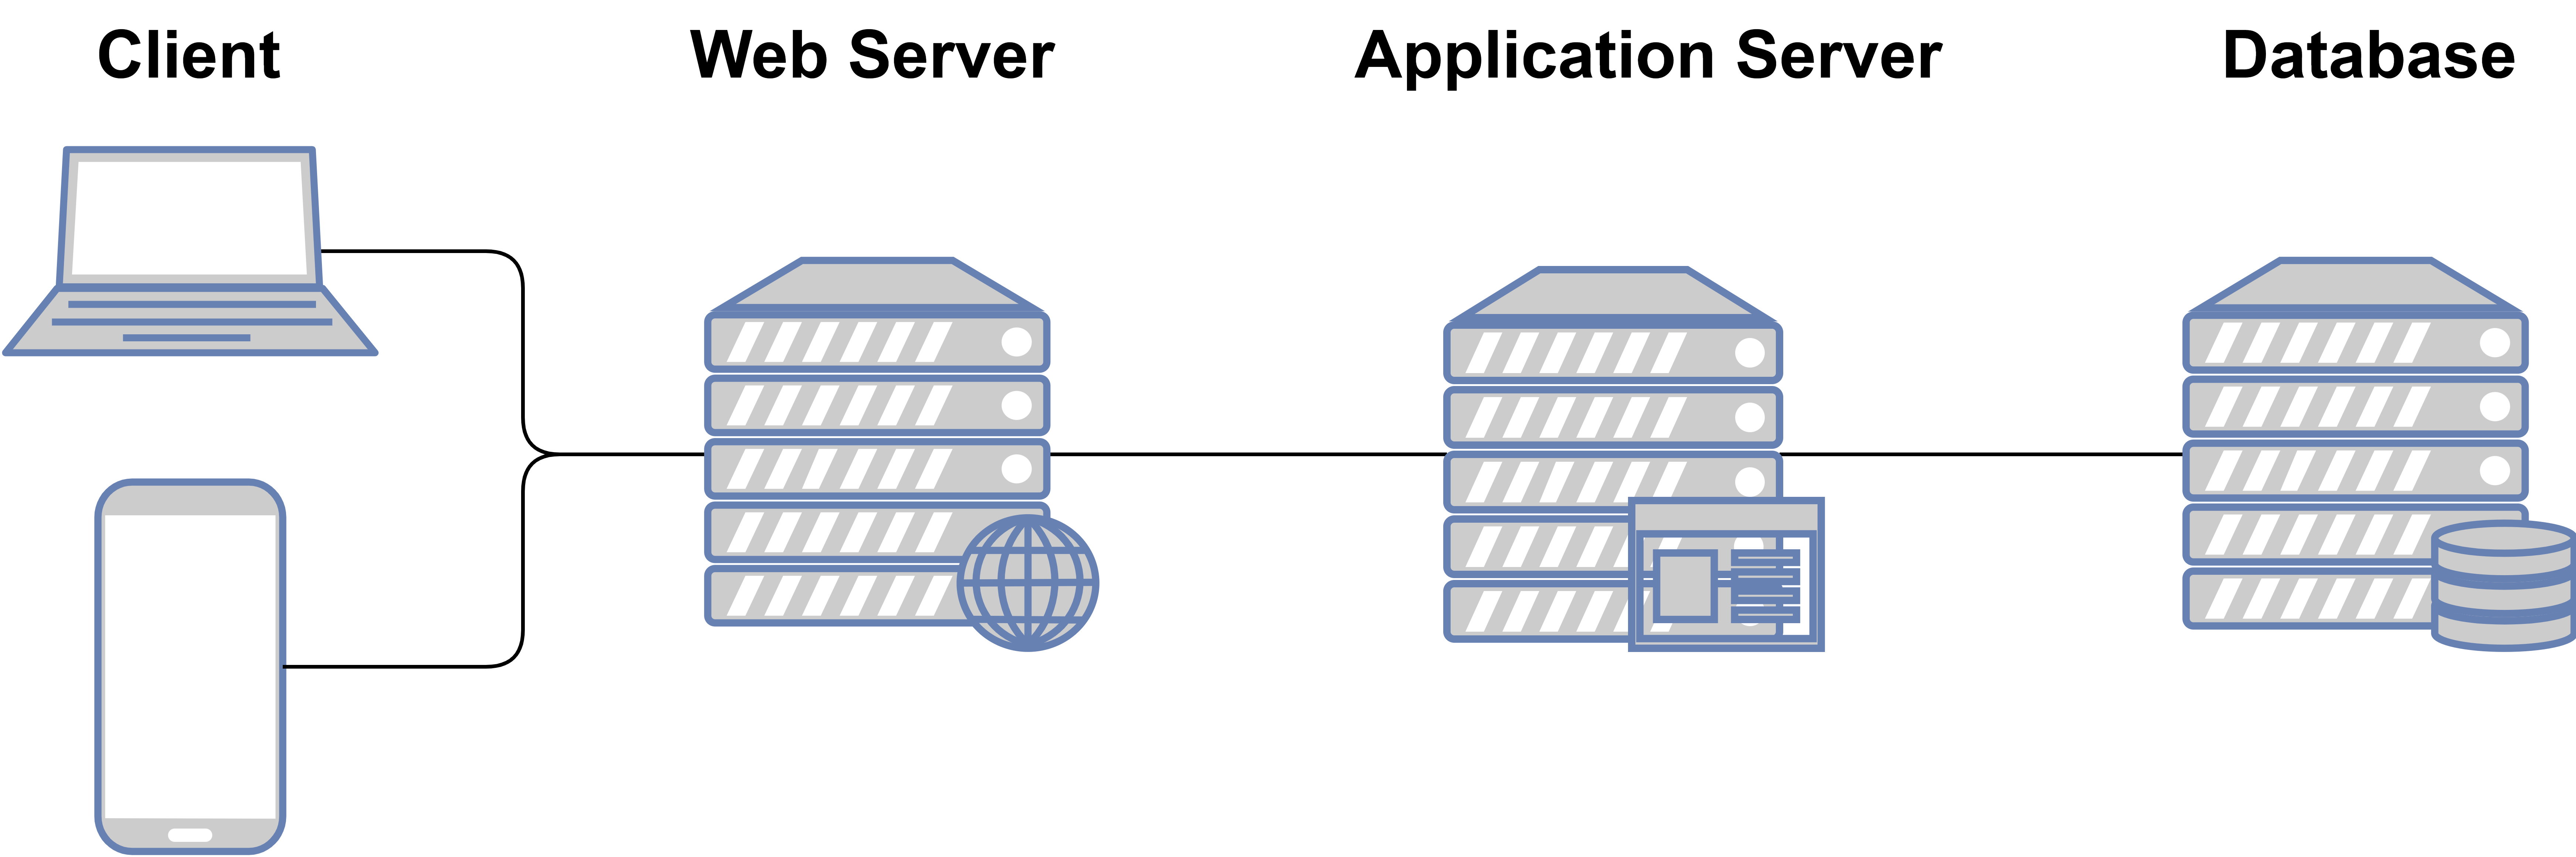
\includegraphics[scale=0.80, center]{assets/3-tier-architecture.png}
        \caption{Three Tier Architecture}
        \label{fig: three_tier_architecture}
    \end{figure}
\end{center}

The system is an application distributed across multiple devices and follows the common client-server paradigm.
The architecture is organized in three logical layers:

\begin{itemize}
    \item \textbf{Presentation Layer (P)}: It's responsible for rendering the application's user interface to the client through the Web Server. It's expressed by a GUI designed to enable the user to interact with the application efficiently.
    \item \textbf{Application Layer (A)}: It's responsible for the business logic of the application. It receives requests from the Presentation Layer, processes them, and then sends back the results to be displayed.
    \item \textbf{Data Layer(D)}: It's in charge of the access to data sources, it provides data through the database and direct it to the other layers. It's also necessary in order to grant a high level of abstraction from the database for an easy to use model.
\end{itemize}

\newpage
\begin{center}
    \begin{figure}[H]
        \includegraphics[scale=0.53, center]{assets/high_level_architecture.png}
        \caption{High Level Architecture}
        \label{fig: high_level_architecture}
    \end{figure}
\end{center}

The system's architecture, as shown in Figure \ref{fig: high_level_architecture}, is composed by a DMZ, that includes the Web and the Mail Server in order to prevent a direct access to the internal system and improve the overall security, and firewalls that divide each newtwork segment.
To reduce computation client side a thin client is used, which allows all the heavy operations to be performed at server side. The Web Server handles the HTTP requests by the users and directs them to the Application Server, while also managing the GoogleMaps API. 
The Application Server communicates with the Database Server and elaborates data following its business logic. The Application server also handles external APIs and services, such as GoogleCalendarAPI, CarAPI, and the exetrnal CPMSs and eMSPs systems.
The Apllication Server's CPMS subsystem will also communicate with its Charging Stations and their relative sockets through the OCPP API, and with the external DSOs through their proprietary API.
The Email Server will manage all the e-mail notification by communicating with the Application Server, The database server is responsible for storing and managing the data that is used by the application. It receives requests for data from the application logic tier, retrieves the requested data from the database, and returns the data to the application logic tier.

\subsection{Component view}
\subsubsection*{General Component View}
\begin{center}
    \begin{figure}[H]
        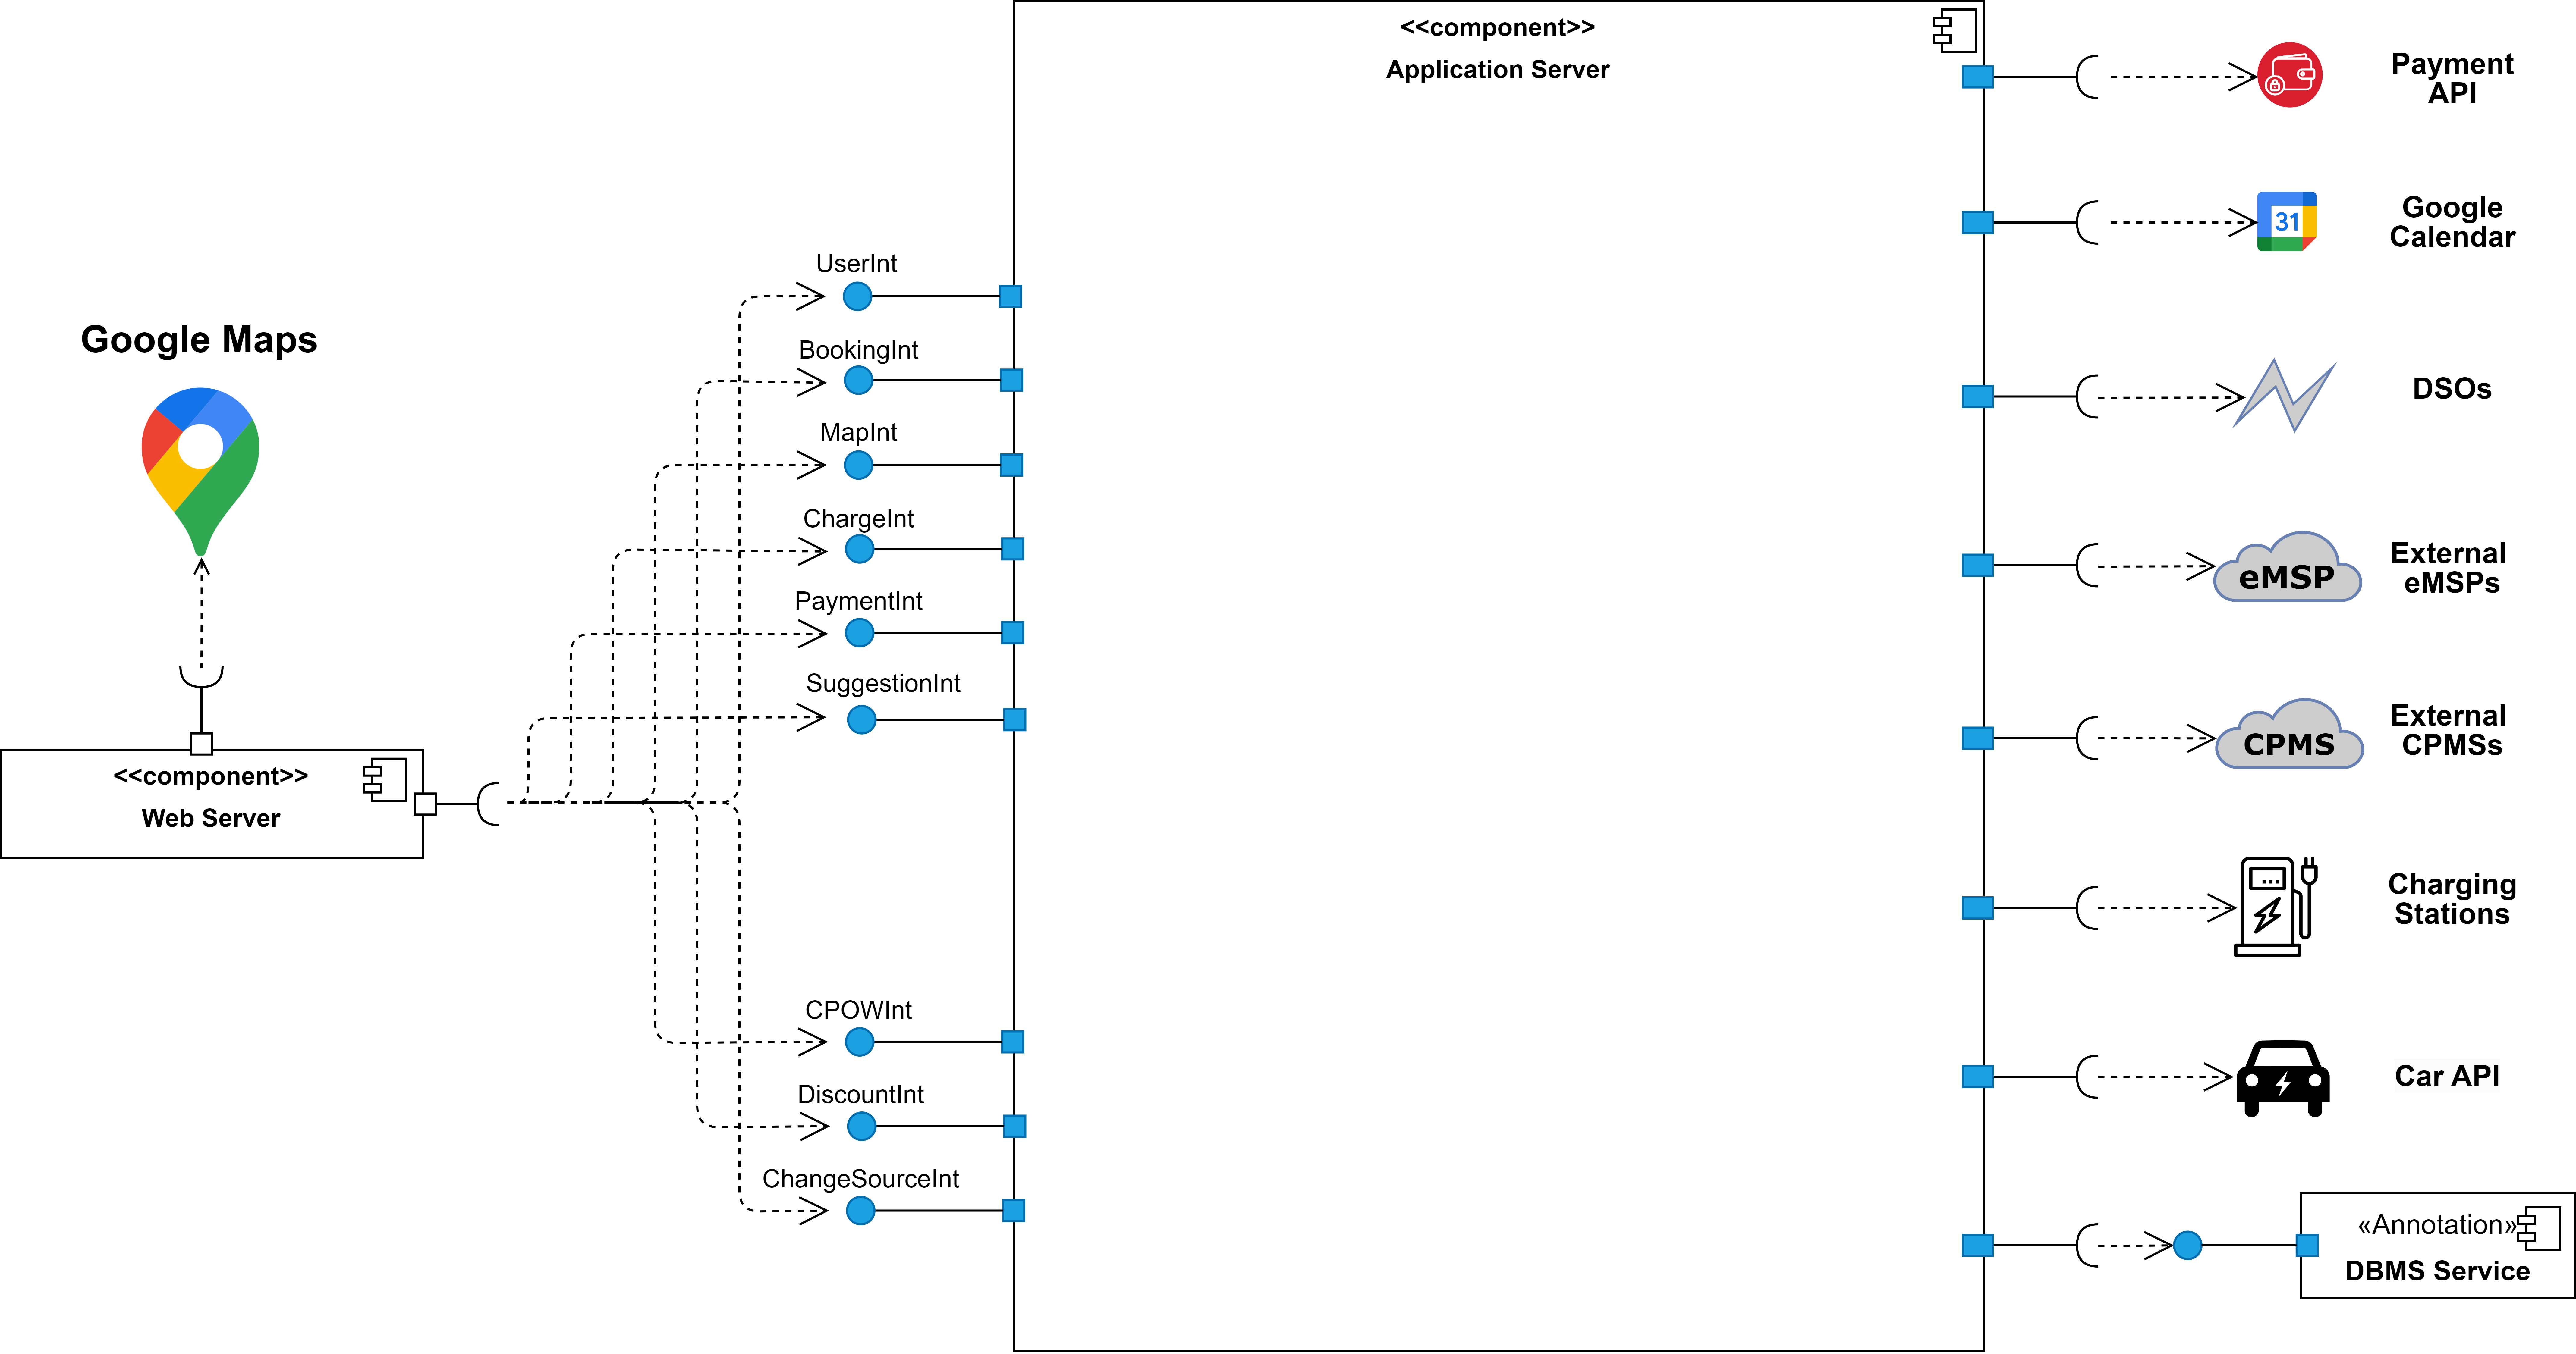
\includegraphics[scale=0.65, center]{assets/general_component_diagram.png}
        \caption{General Component Diagram}
        \label{fig: general_component_view}
    \end{figure}
\end{center}

This image gives a high level representation of the components of the system.
In the scheme the application server is represented by an empty box, since a complete description will be provided in the next section. On the left the interfaces between the web server and the application server are shown; these basically represent the main functionalities requested by the client applications. On the opposite site the external interfaces are presented, among which there are the interfaces to other CPMSs and to the charging stations. Additionally, there's also the DBMS iterface, which manages the DBMS service and handles all communications between the Applicantion server and the Database server. 

\subsubsection*{Application Server Component View}
\begin{center}
    \begin{figure}[H]
        \includegraphics[scale=0.33, center]{assets/application-server-component-diagram.png}
        \caption{Application Server Component Diagram}
        \label{fig: application_server_component_view}
    \end{figure}
\end{center}

The following component diagram gives a detailed view of the Application Server. It shows the internal structure and the interaction between the components.
External elements in the diagram are represented in a simplified way.
\\
\textbf{eMSP subsystem}
\begin{itemize}
    \item \textbf{AccountManager}: Handles all the basic requests that a client can make. Among those the \textit{AuthenticationService} manages the authentication process (log in, log out, sign up). All the specific functionalities are then provided once the user logs in.
    \item \textbf{eMSP\_UserManager}: It manages all the services available to the eSMP subsystem's users. Various services are then handled by other components, for example the \textit{BookingService} is handled by the \textit{BookingManager}, which communicates through the OCPI component with the CPMSs. Most services also communicate with the Database through an interface.
    \item \textbf{BookingManager}: It handles all the booking requests made by the clients and is responsible for sending the requests to the CPMS through the OCPI component.
    \item \textbf{ChargingProcessManager}: This component manages the charging process service of the user's car, in particular it provides updated informations about the charging status while interacting with the OCPI component to retrive informations and also managing the start and stop charging functions.
    \item \textbf{ChargingStationManager}: This component  handles the Charging Stations general informations and status to be displayed through the \textit{InteractiveMapService}. To do so it interacts with the OCPI component to retrive all the info from the CPMSs.
    \item \textbf{PaymentManager}: It manages the paymentService. It interacts with the external component \textit{Payment}.
    \item \textbf{SuggestionManager}: It handles the service that generates suggestions for the users on when to charge the car. In order to do that it communicates with the \textit{EVmanager} and with the \textit{CalendarManager} to get all the informations needed to formulate suggestions, in particular the user's schedule and the car battery status.
    \item \textbf{CalendarManager}: This component manages the information relative to the user's schedule for the \textit{SuggestionService}. To do so it interfaces with the external component \textit{Calendar}.
    \item \textbf{EVManager}: This component handles the information relative to the user EVs' battery status and location for the \textit{SuggestionService}. To do so it interfaces with the external component \textit{CarAPI}. It also manages the registration of new EVs through the \textit{EV Service}.
    \item \textbf{OCPI}: It handles the interaction with all the CPMSs, it sends and retrives data from them. All the components that require an interaction with the CPMSs are connected to it.
\end{itemize}
\textbf{CPMS subsystem}
\begin{itemize}
    \item \textbf{AccountManager}: This component, similar to the one in the eMSPsubsystem, handles the authentication process. 
    \item \textbf{DiscountManager}: It handles the addition and deletion of offers and manages the \textit{DiscountService}.
    \item \textbf{ChargingStation Manager}: This component manages the information about the charging stations and the services related to them, in particular \textit{ChangeSourceService} and \textit{ChargingStationService}.
    \item \textbf{OCPI}: It manages the connection with eMSPs, sending and receiving data from them. Both the \textit{DiscountManager} and the \textit{Charging Station Manager} are connected to this component in order to send information to the eMSPs.
    \item \textbf{OCPP}: This component handles the connection with the charging stations, sending data regarding offers, changes in the energy source and charging sessions. It receives data from the charging stations regarding their current status. All the components that need to communicate with the charging stations interact with this component.
    \item \textbf{DSO Manager}: This component manages the communication with external DSOs. All components and services that require communication with a DSO, for example the \textit{Change Source Service} managed by the \textit{Charging Station Manager}, interact with this component.
\end{itemize}
\subsubsection*{Web Server Component View}
Regarding the Web Server the main components are:
\begin{itemize}
    \item \textbf{first component}: description of component.
\end{itemize}

\newpage

\subsection{Deployment view}
\begin{center}
    \begin{figure}[H]
        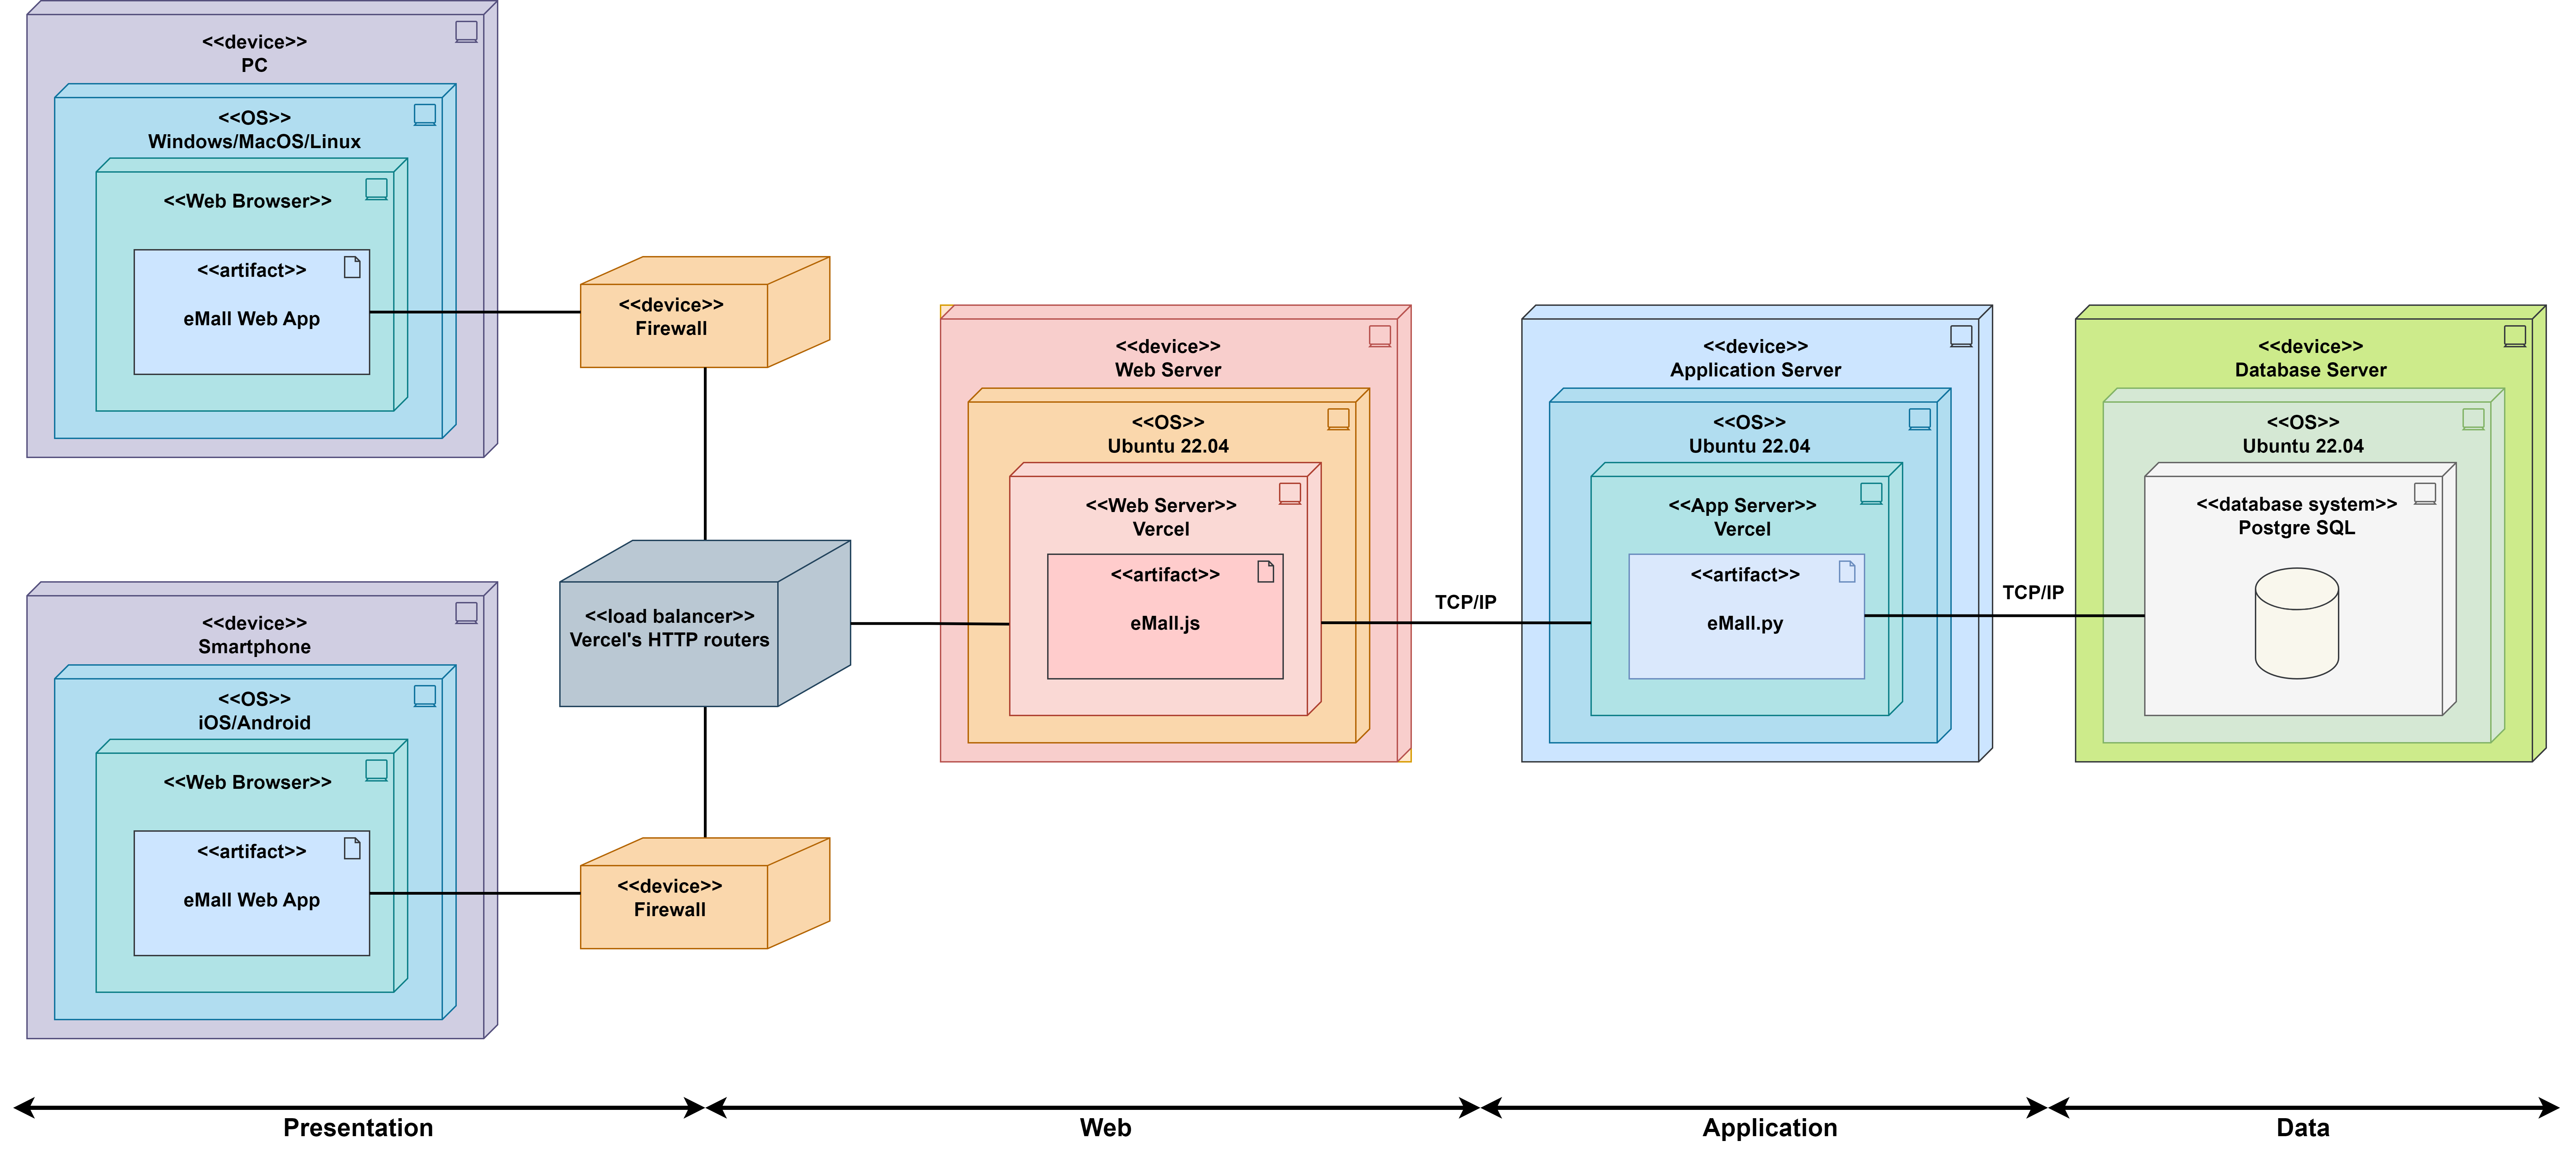
\includegraphics[scale=0.35, center]{assets/archimate.png}
        \caption{Deployment Diagram}
        \label{fig: deployment_diagram}
    \end{figure}
\end{center}

The deployment diagram in \textit{Figure (\ref{fig: deployment_diagram})} shows how the various components of the web application are deployed across the network, including the web server, application server, and database server. It also shows the relationships and the flow of data between them.
The devices shown are:
\begin{itemize}
    \item \textbf{PC/Smartphone}: The user's device, where the web application is displayed. They can be used to access the web application and to interact with it through the web browser and the HTTPS protocol.
    \item \textbf{Firewall}: Protects the network from unauthorized access. It is used to filter the incoming and outgoing traffic.
    \item \textbf{Load Balancer}: It is used to distribute the incoming traffic to the web servers and it guarantees the availability of the web application and the scalability of the system. Since the project will be hosted on Vercel it will use thier provided load balancer.
    \item \textbf{Web Server}: Hosts the web application and provides the rendered HTML and CSS web pages to the user's device. It is also responsible for the HTTPS protocol by routing the traffic to the application server, and the Google Maps API, which is used to display the interactive map.\\In order to provide the best performance, the web server will be hosted on Vercel, which is a cloud platform that provides serverless deployment and global distribution of the web application.
    \item \textbf{Application Server}: It is responsible for the business logic of the web application by managing all the requests coming from the web server. It also interacts with the database server, to retrieve and store data, and all the external services such as the Google Calendar API, the Car API, the Payment API, the OCPI and the OCPP.\\ The applicaiton server will host both the eMSP and the CPMS subsystems.
    \item \textbf{Database Server}: It runs the database that stores all the data of the web application. We will use a PostgreSQL database in order to easily manage the relations between the tables and the incoming queries.
\end{itemize}
\newpage

\subsection{Runtime view}

In this section we list some relevant use cases of the system, represented through sequence diagrams. 
In some diagrams, interactions like the login phase, returning to home page or retrieve the same kind of data were omitted for the sake of clarity.

\newpage
\underline{\textbf{Shared diagrams}}\\
\textbf{Sign Up}
\begin{center}
    \begin{figure}[H]
        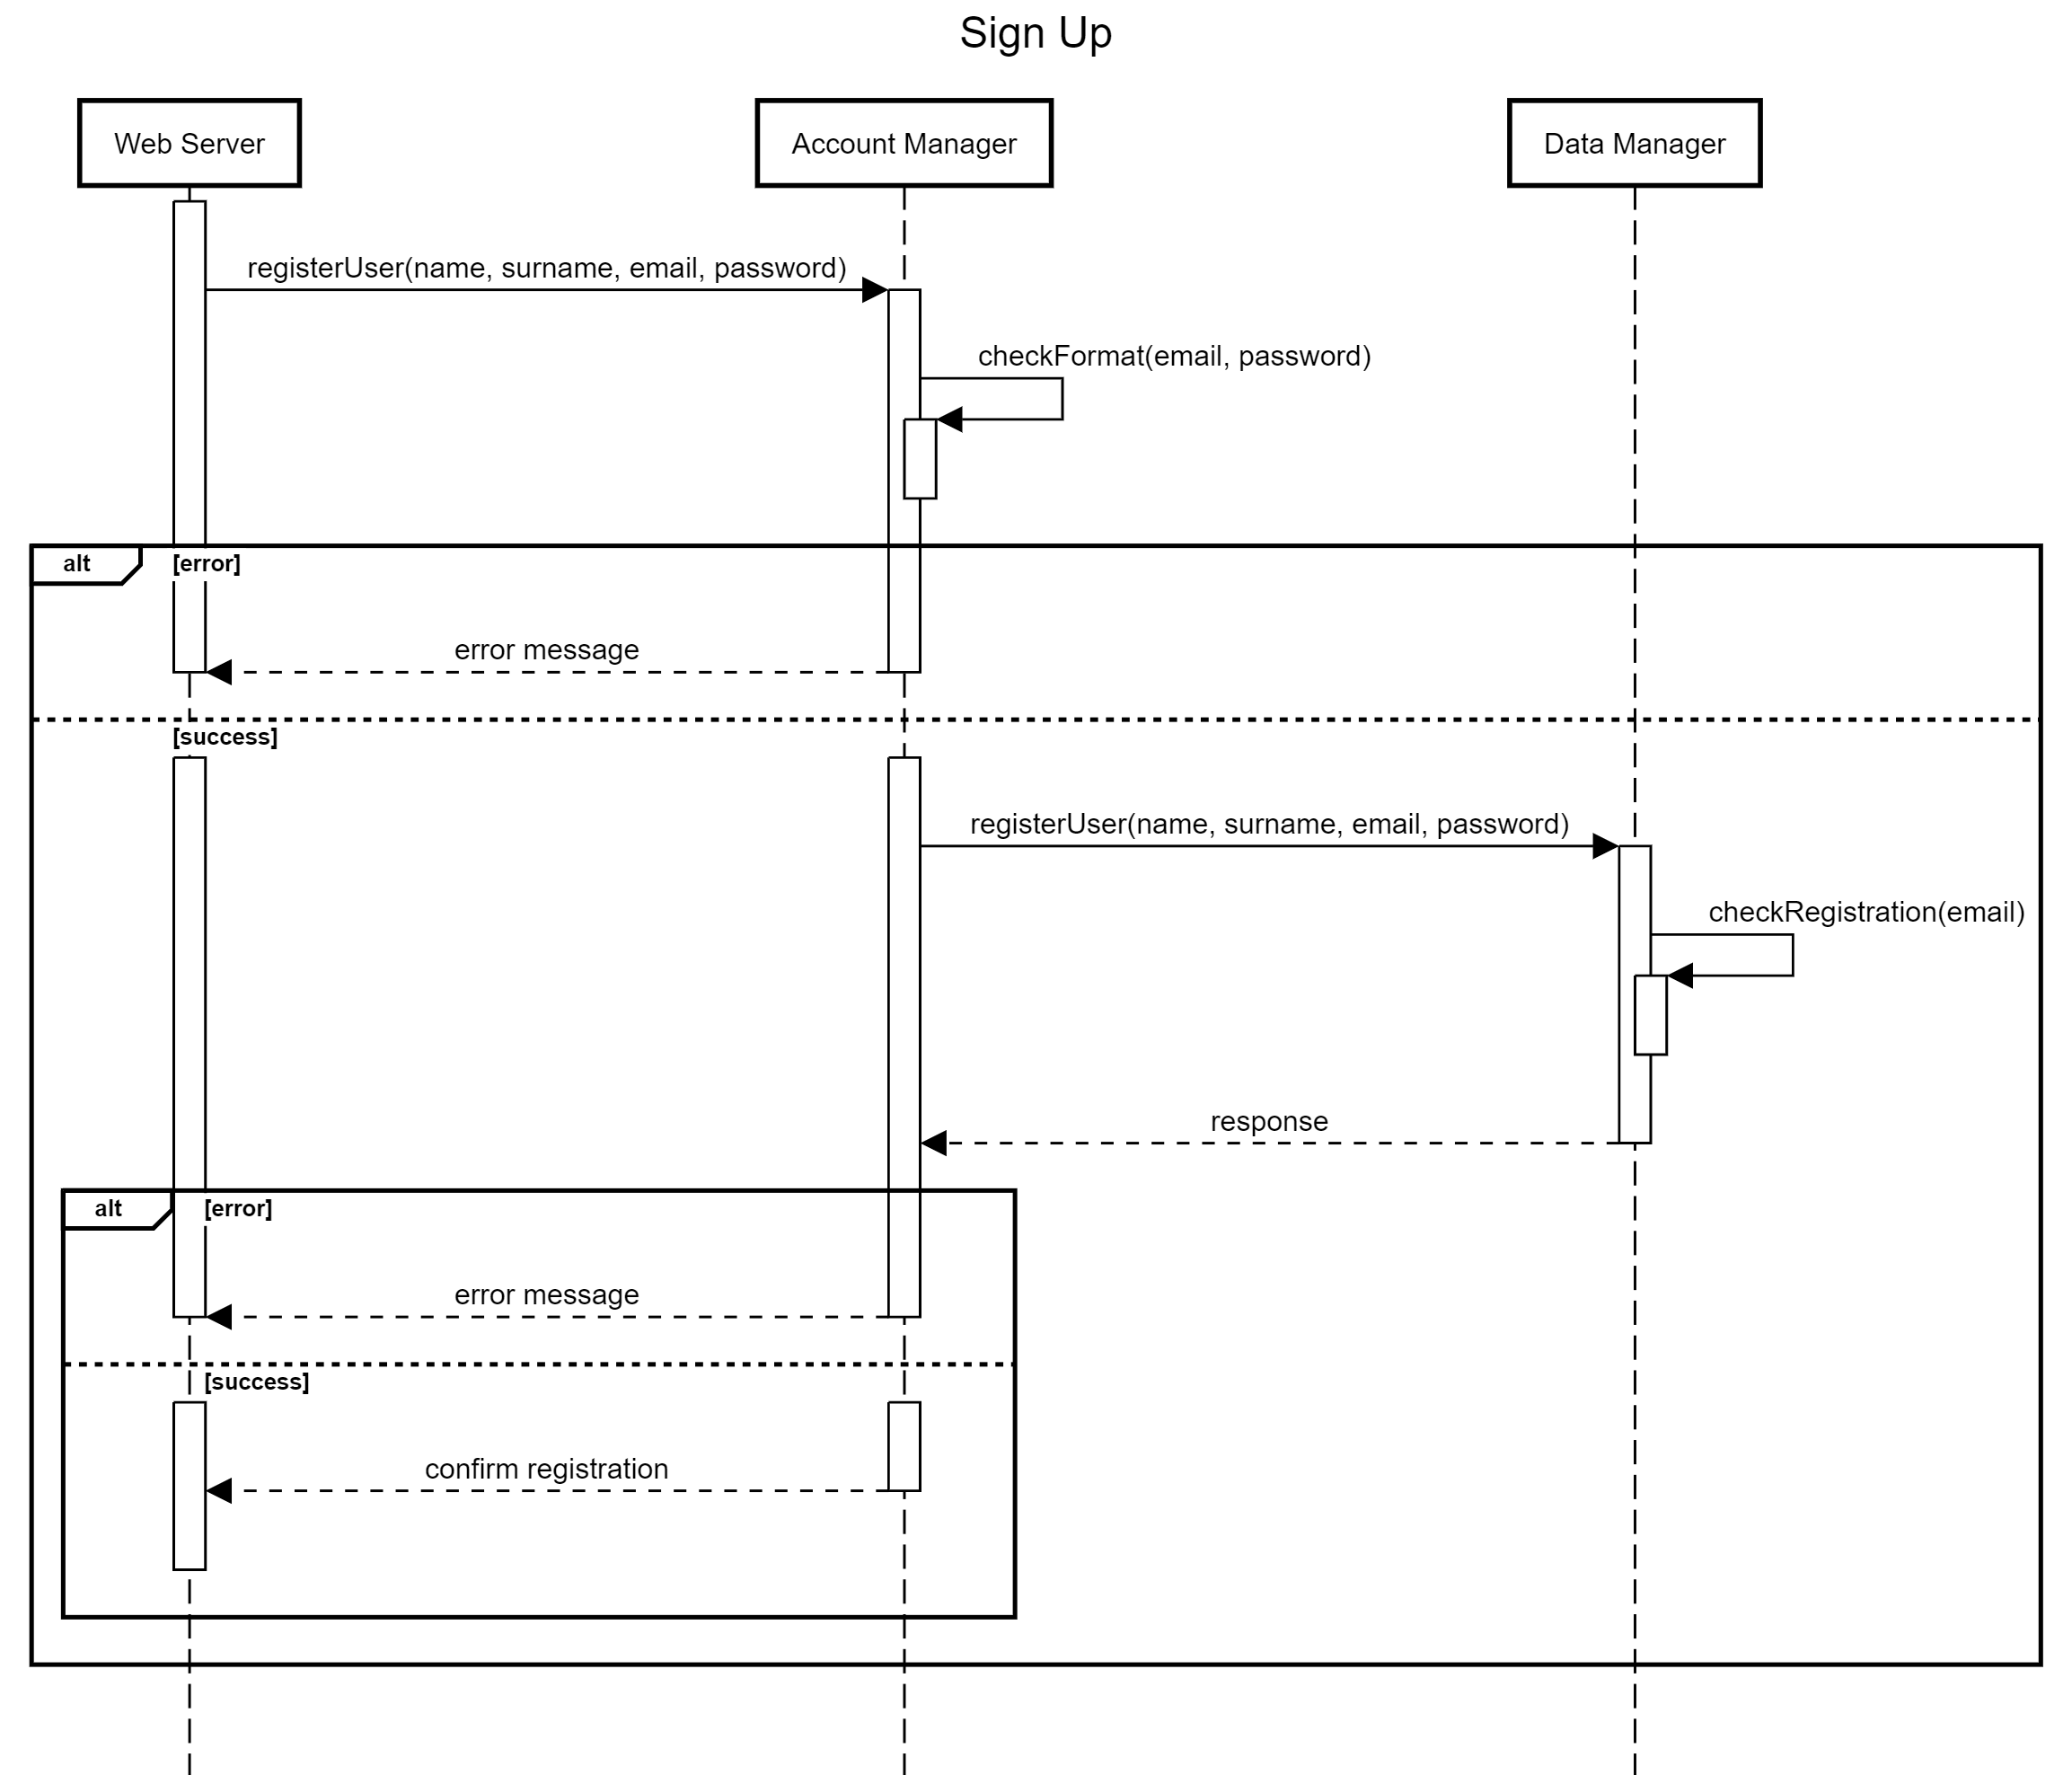
\includegraphics[scale=0.15, center]{assets/sequenceDiagrams/shared signup.png}
        \caption{Sign Up}
        \label{fig:signup}
    \end{figure}
\end{center}
The Sign-up phase consists in the user action of inserting their personal data in the sign-up fields, then the system checks if the email (unique key in the database) is already present in the database.
If it's not, the user can sign up and use the system functionalities available for that particular type of account depending if he's registering through the eMSP or the CPMS.

\newpage

\textbf{Log In}
\begin{center}
    \begin{figure}[H]
        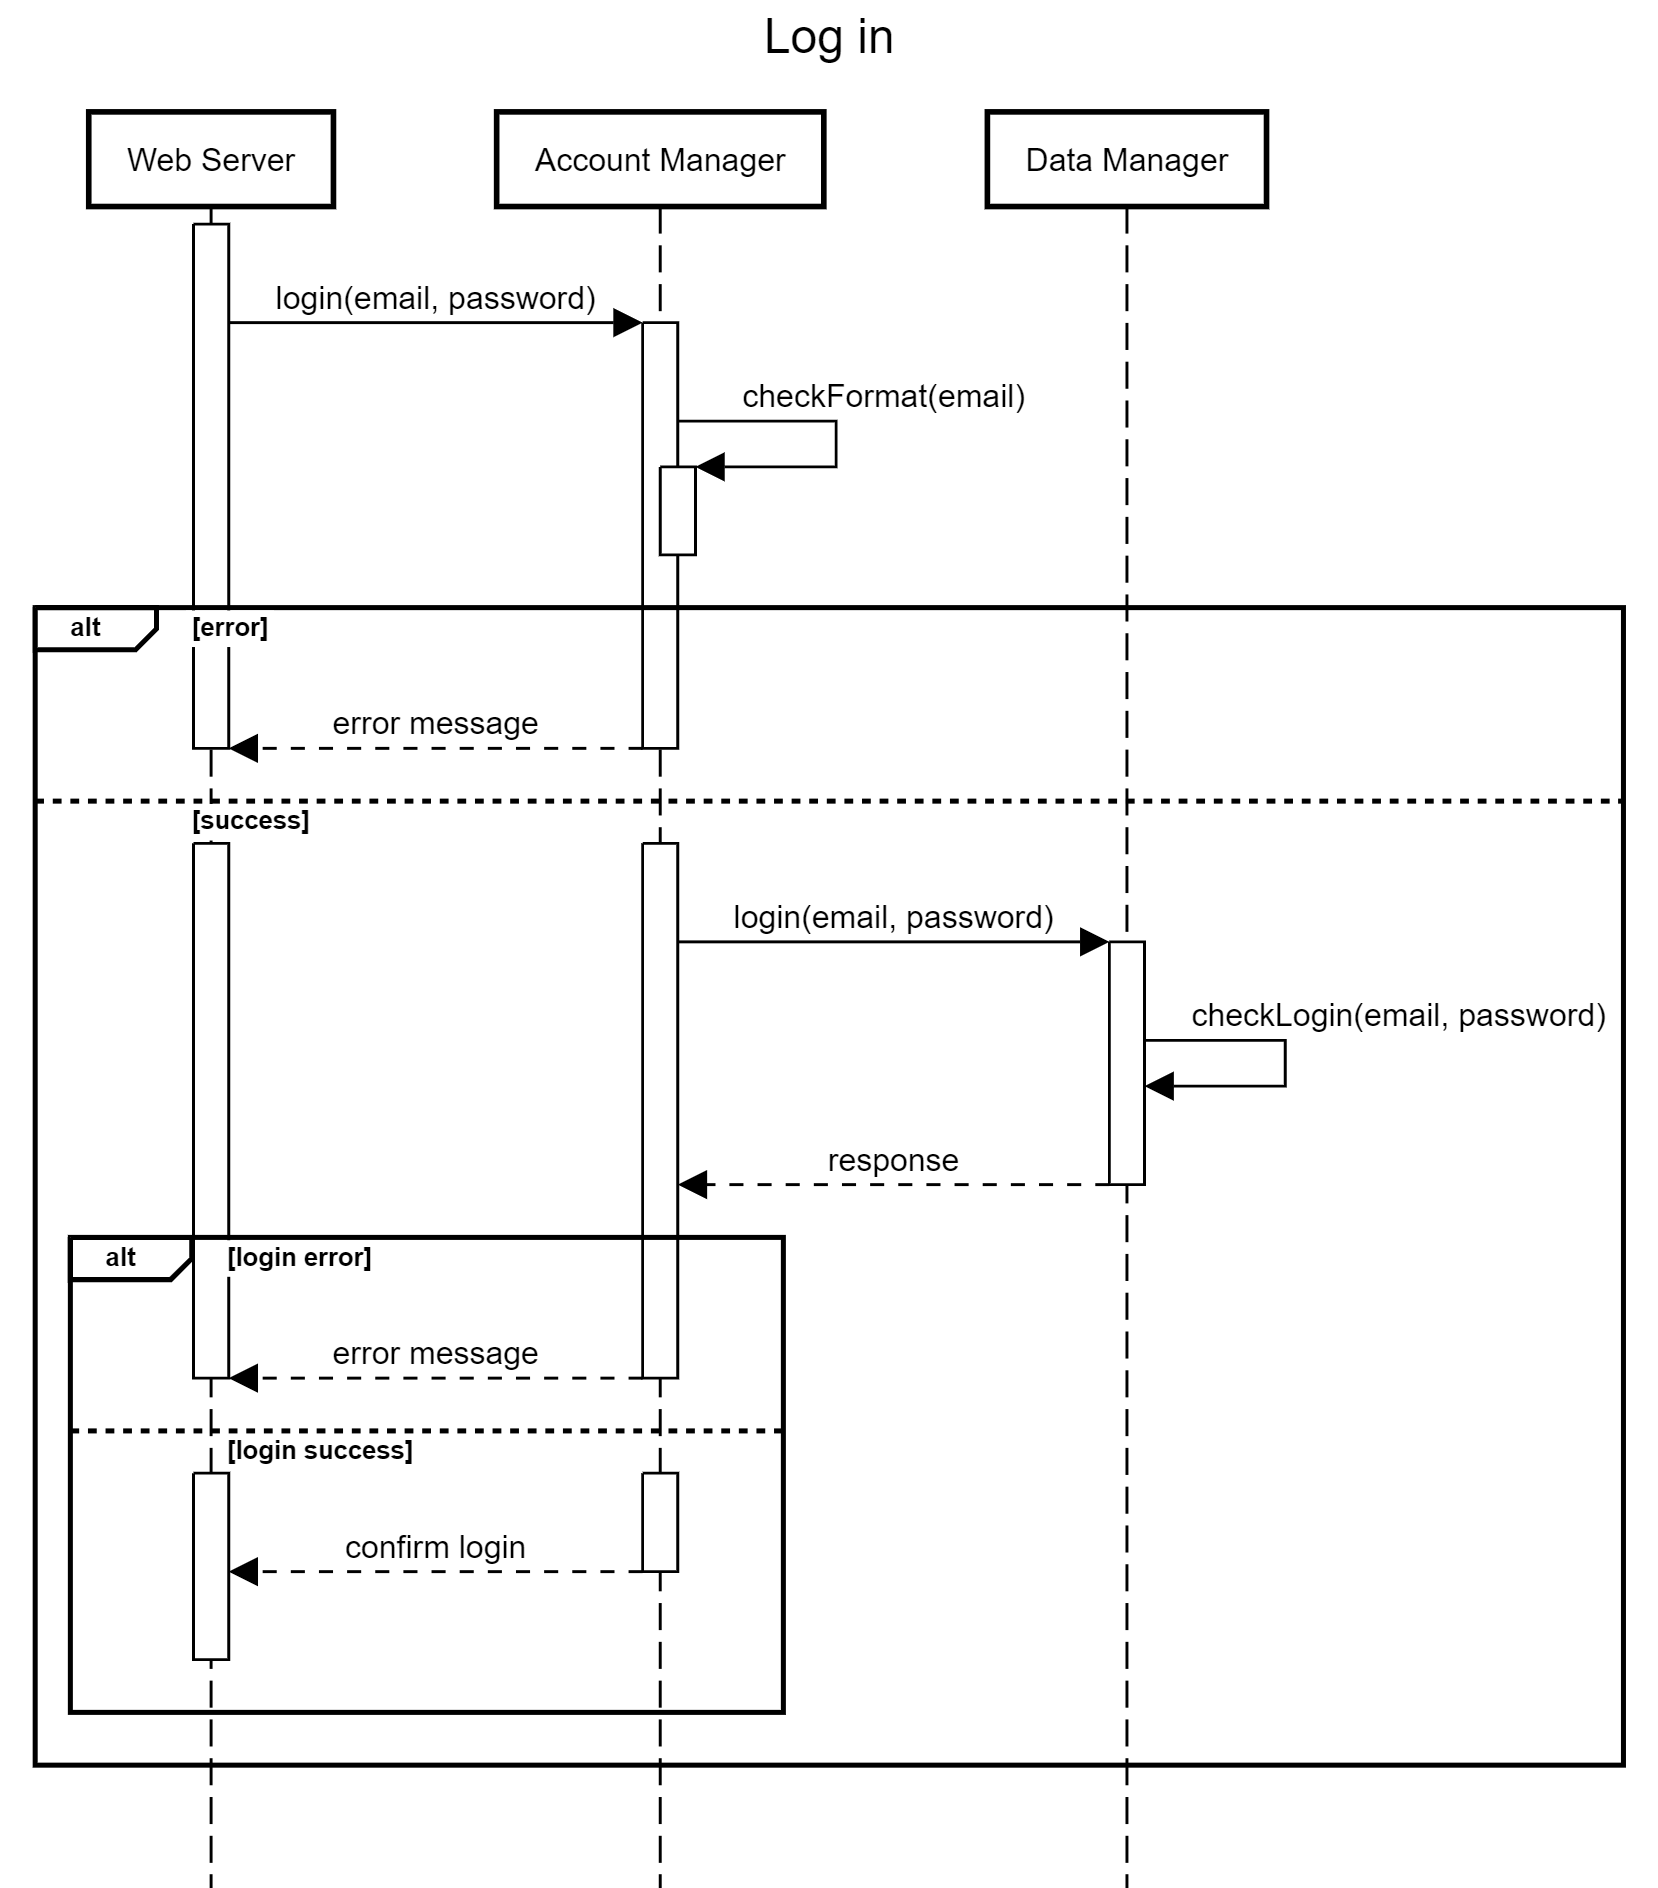
\includegraphics[scale=0.2, center]{assets/sequenceDiagrams/shared login.png}
        \caption{Log In}
        \label{fig: login}
    \end{figure}
\end{center}

The Log In phase consists in the user action of inserting their email (unique key in the database) and password in the login fields, then the system checks if the pair corresponds to a user entry in the database.
In case of success, the user can log-in and use the system functionalities available for that particular type of account depending if he's logging in through the eMSP or the CPMS.

\newpage
\underline{\textbf{User diagrams}}\\

\textbf{View Nearby Stations}
\begin{center}
    \begin{figure}[H]
        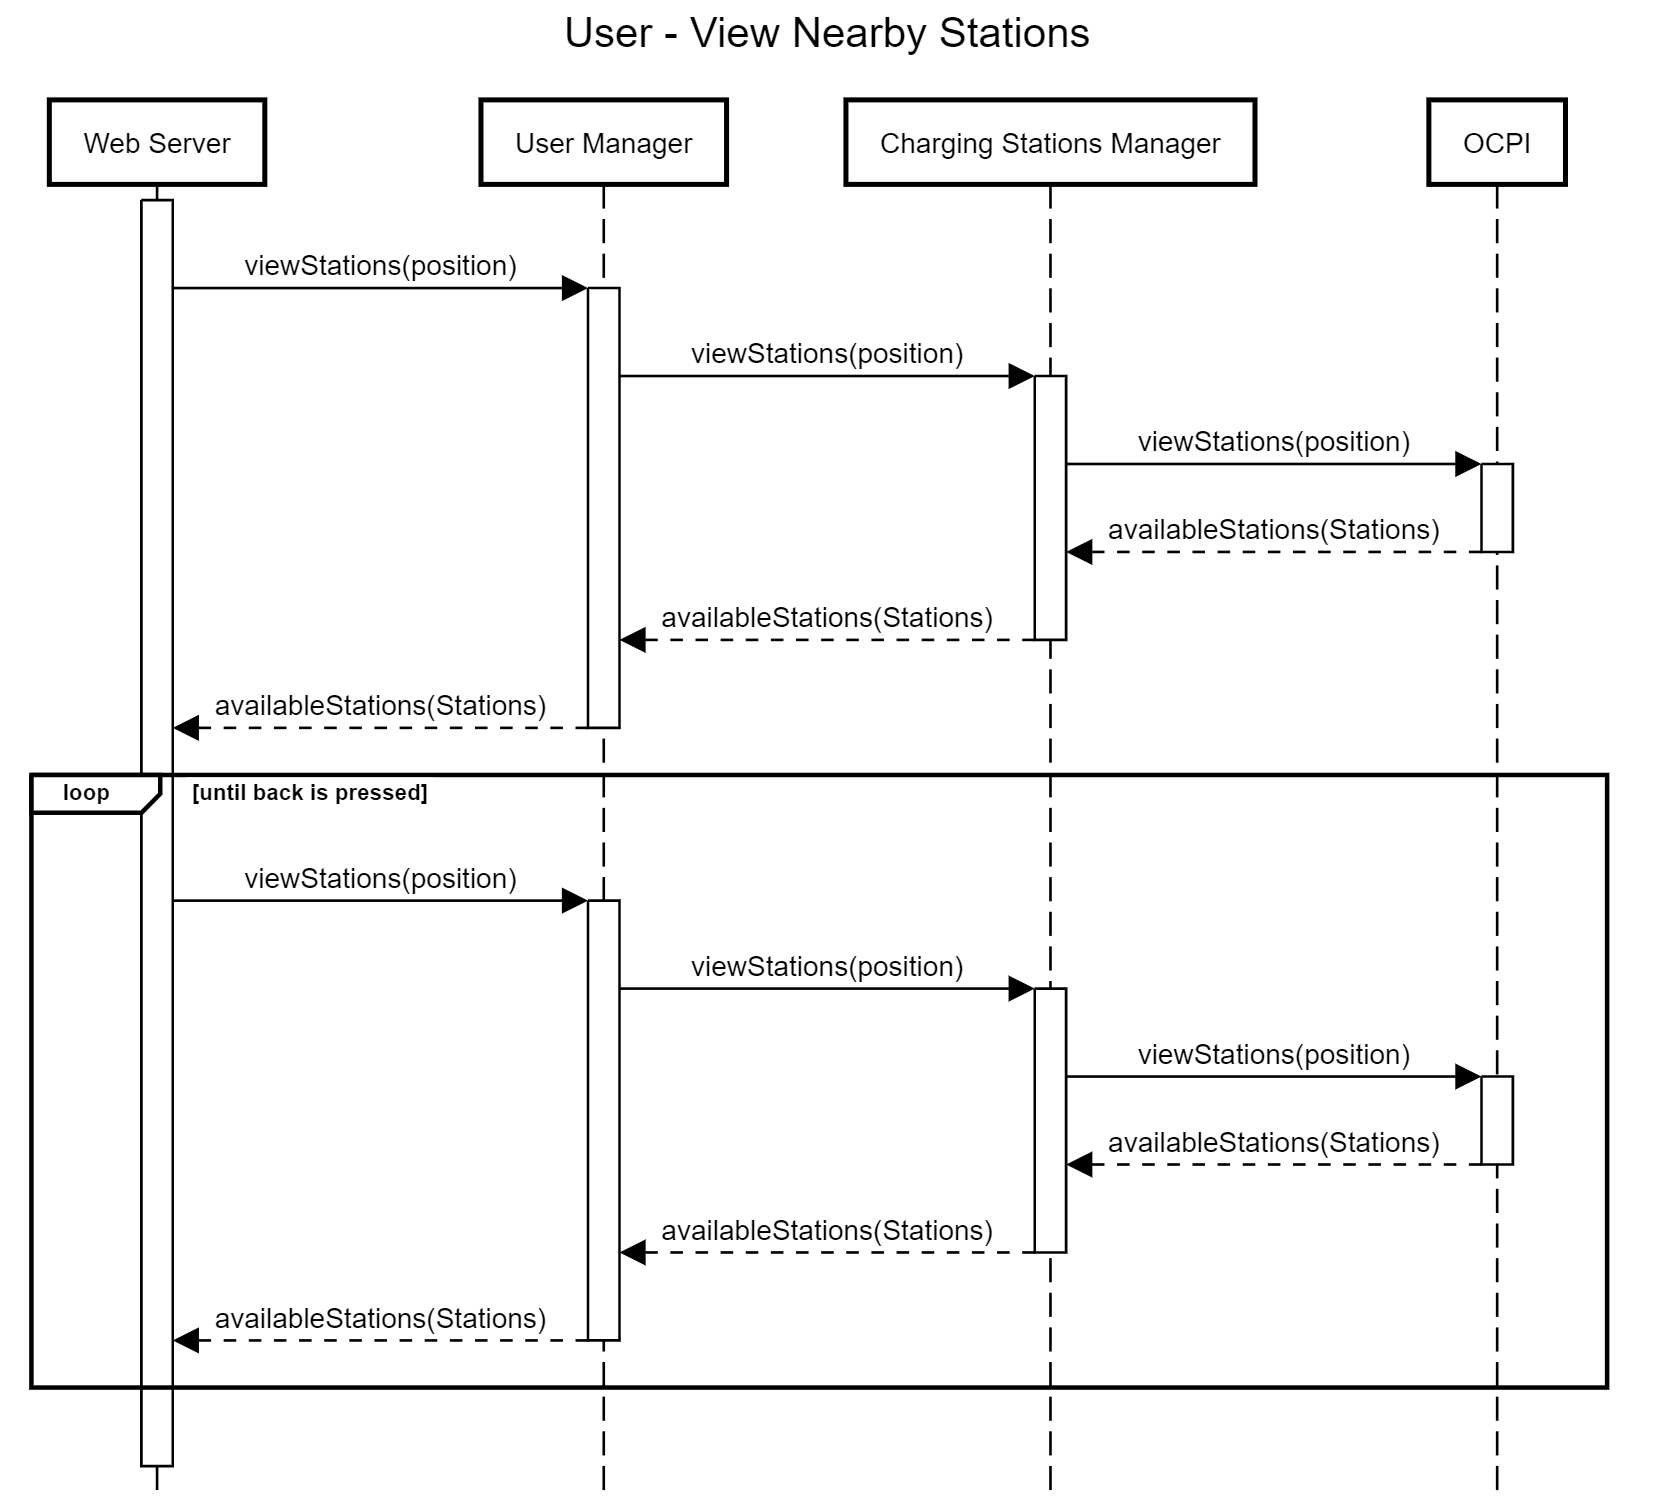
\includegraphics[scale=0.15, center]{assets/sequenceDiagrams/User View Nearby Stations.png}
        \caption{View Nearby Stations}
        \label{View Nearby Stations}
    \end{figure}
\end{center}
The view nearby stations is the process through which the interactive map is updated when the user is inside the webapp. In this diagram it is assumed the user is already on the interactive map part.
Upon detecting the user's movement on the map, the server retrieves the new stations that must be loaded caused by the movement. This process is repeated while the user is navigating on the map, and ends only when the user exits it.

\newpage

\textbf{Delete a Booking}
\begin{center}
    \begin{figure}[H]
        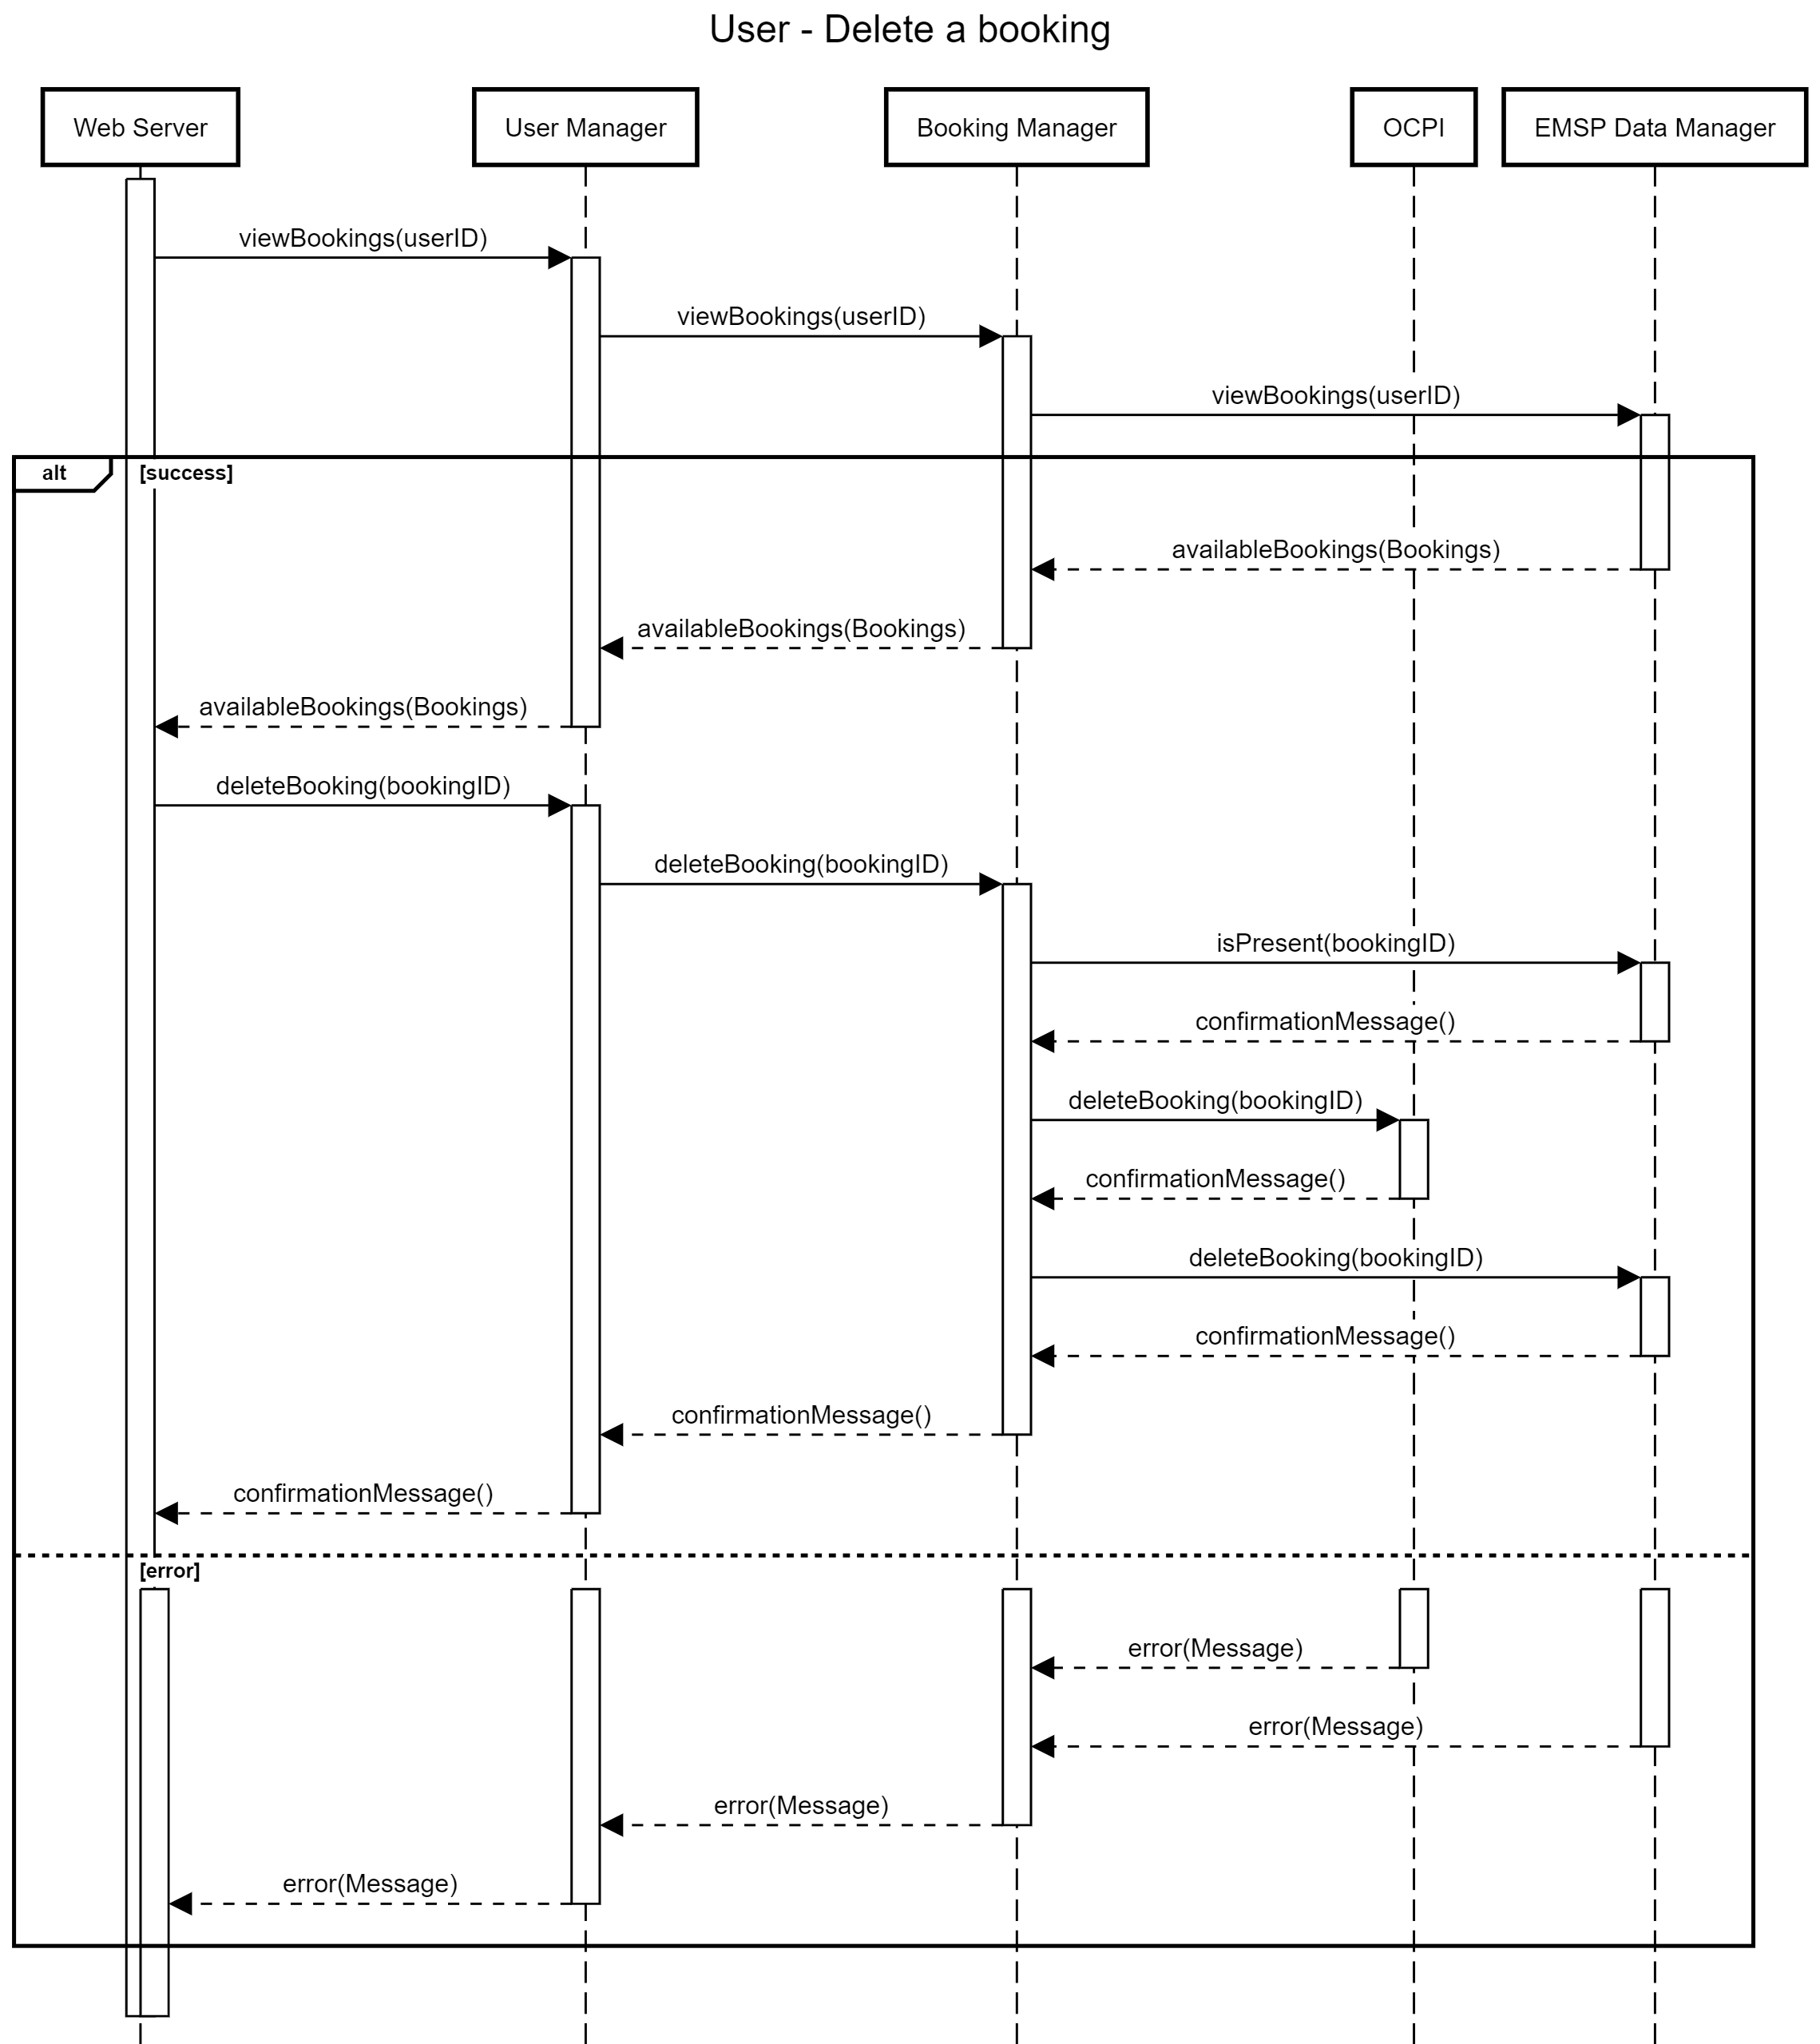
\includegraphics[scale=0.15, center]{assets/sequenceDiagrams/User delete bookings.png}
        \caption{Delete a Booking}
        \label{Delete Booking}
    \end{figure}
\end{center}
In the first part of the sequence the user is viewing his bookings list and clicks on "Delete" on one of them. The id of said selected booking is then sent to process the deletion request.
Firstly, a check by the Booking Manager is done to assure the bookingID sent is actually present on the database of that user's bookings. If present, the Booking Manager proceeds to firstly delete the booking from the 
interested station(communicating with OCPI) then deleting it from the user's bookings on the database (communicating with eMSP Data Manager again).
 For the sake of readability, all errors are pushed to the end and will be furhter explained here by text. The first error that can happen is caused by the user not having any active bookings.
 The second possible error is caused by the first check in case the bookingID that has to be deleted doesn't exist in the database.
 Lastly, an error could be caused by the requested booking not existing on the OCPI. 

\newpage
\textbf{Make a Booking}
 \begin{center}
    \begin{figure}[H]
        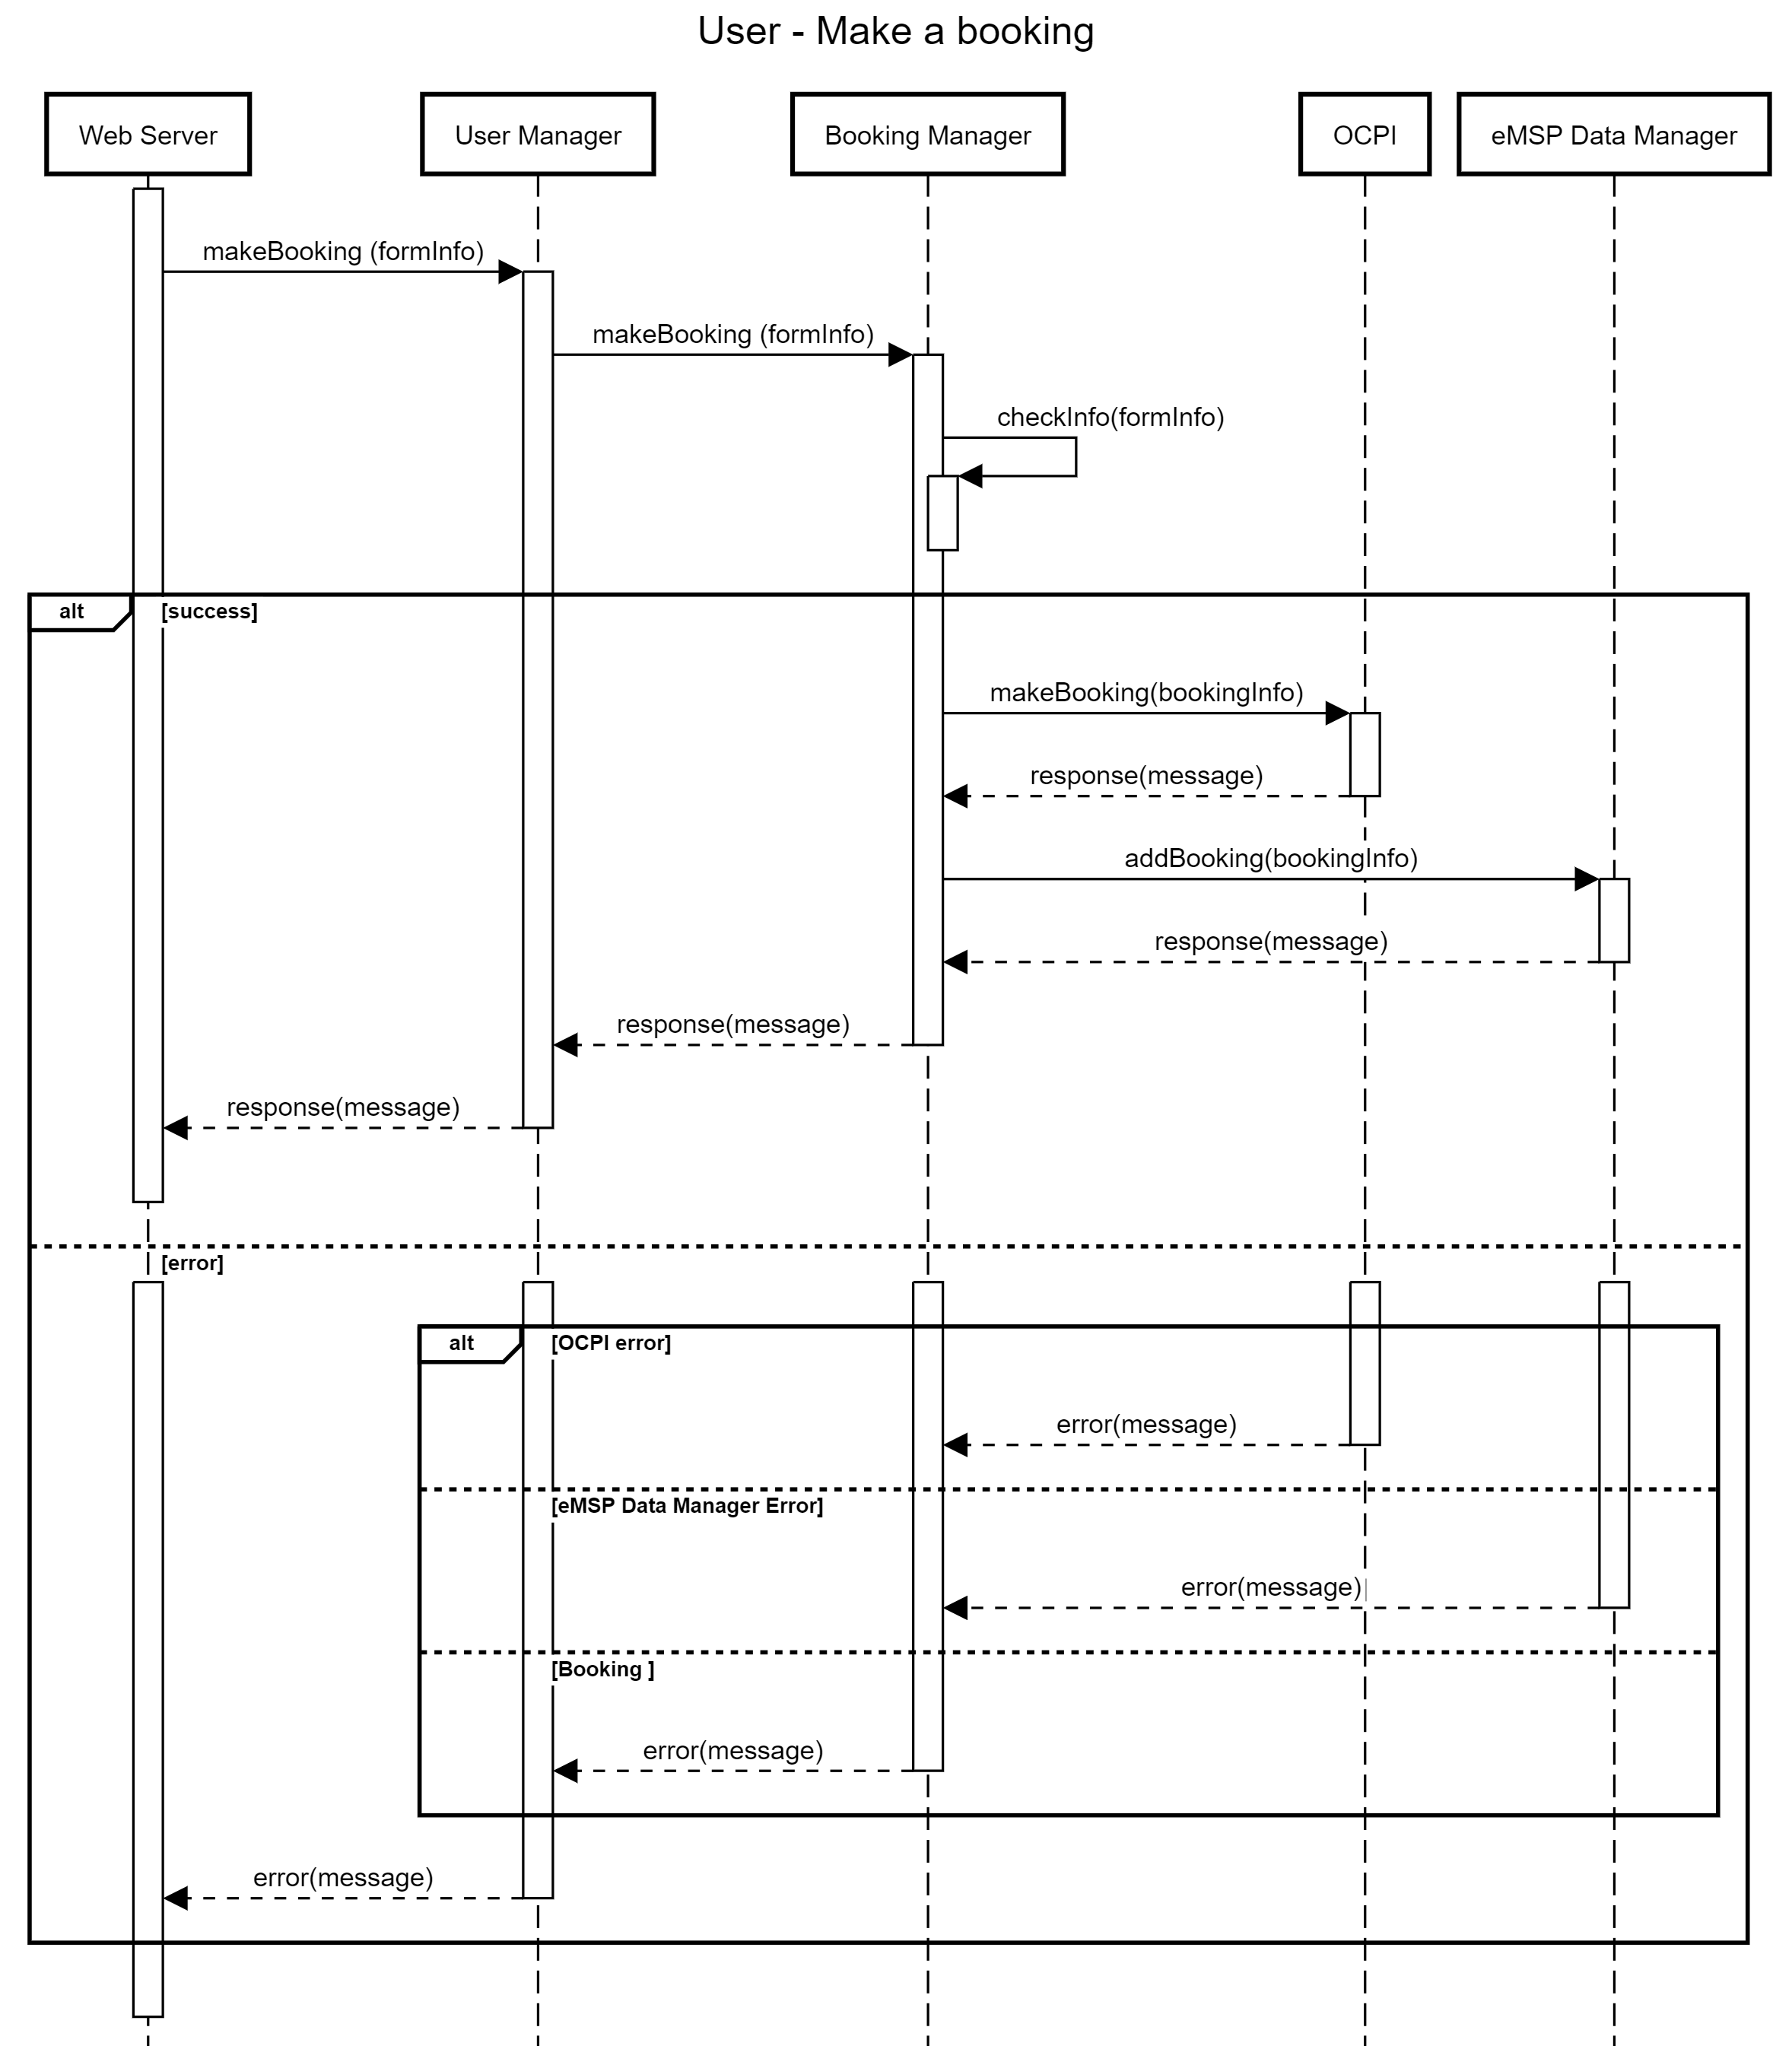
\includegraphics[scale=0.15, center]{assets/sequenceDiagrams/User Make Booking.png}
        \caption{Make a Booking}
        \label{Make Booking}
    \end{figure}
\end{center}
This sequence displays how a user is able to insert a new booking from a form. The form is firstly sent to the Booking Manager, where a check for the validity of all the information is done. If it is all valid, the info is extrapolated and the 
booking is communicated to the OCPI. The booking info is later saved on the database through the eMSP Data Manager. For the sake of readability, all errors are collapsed in the end and explained here.
The first possible error is caused by checkInfo(), if the data inserted by the user is invalid. Lastly, an error could be raised by the OCPI if the booking doesn't go through for any reason. We assume the addition of the booking to the database doesn't cause errors.
\newline

\textbf{Book from map}\newline
We decided not to show book from map as it is basically the same as Make a Booking: it is still a form that has some fields precompiled when the button is pressed on the map.
\newpage

\textbf{Charging process}
\begin{center}
    \begin{figure}[H]
        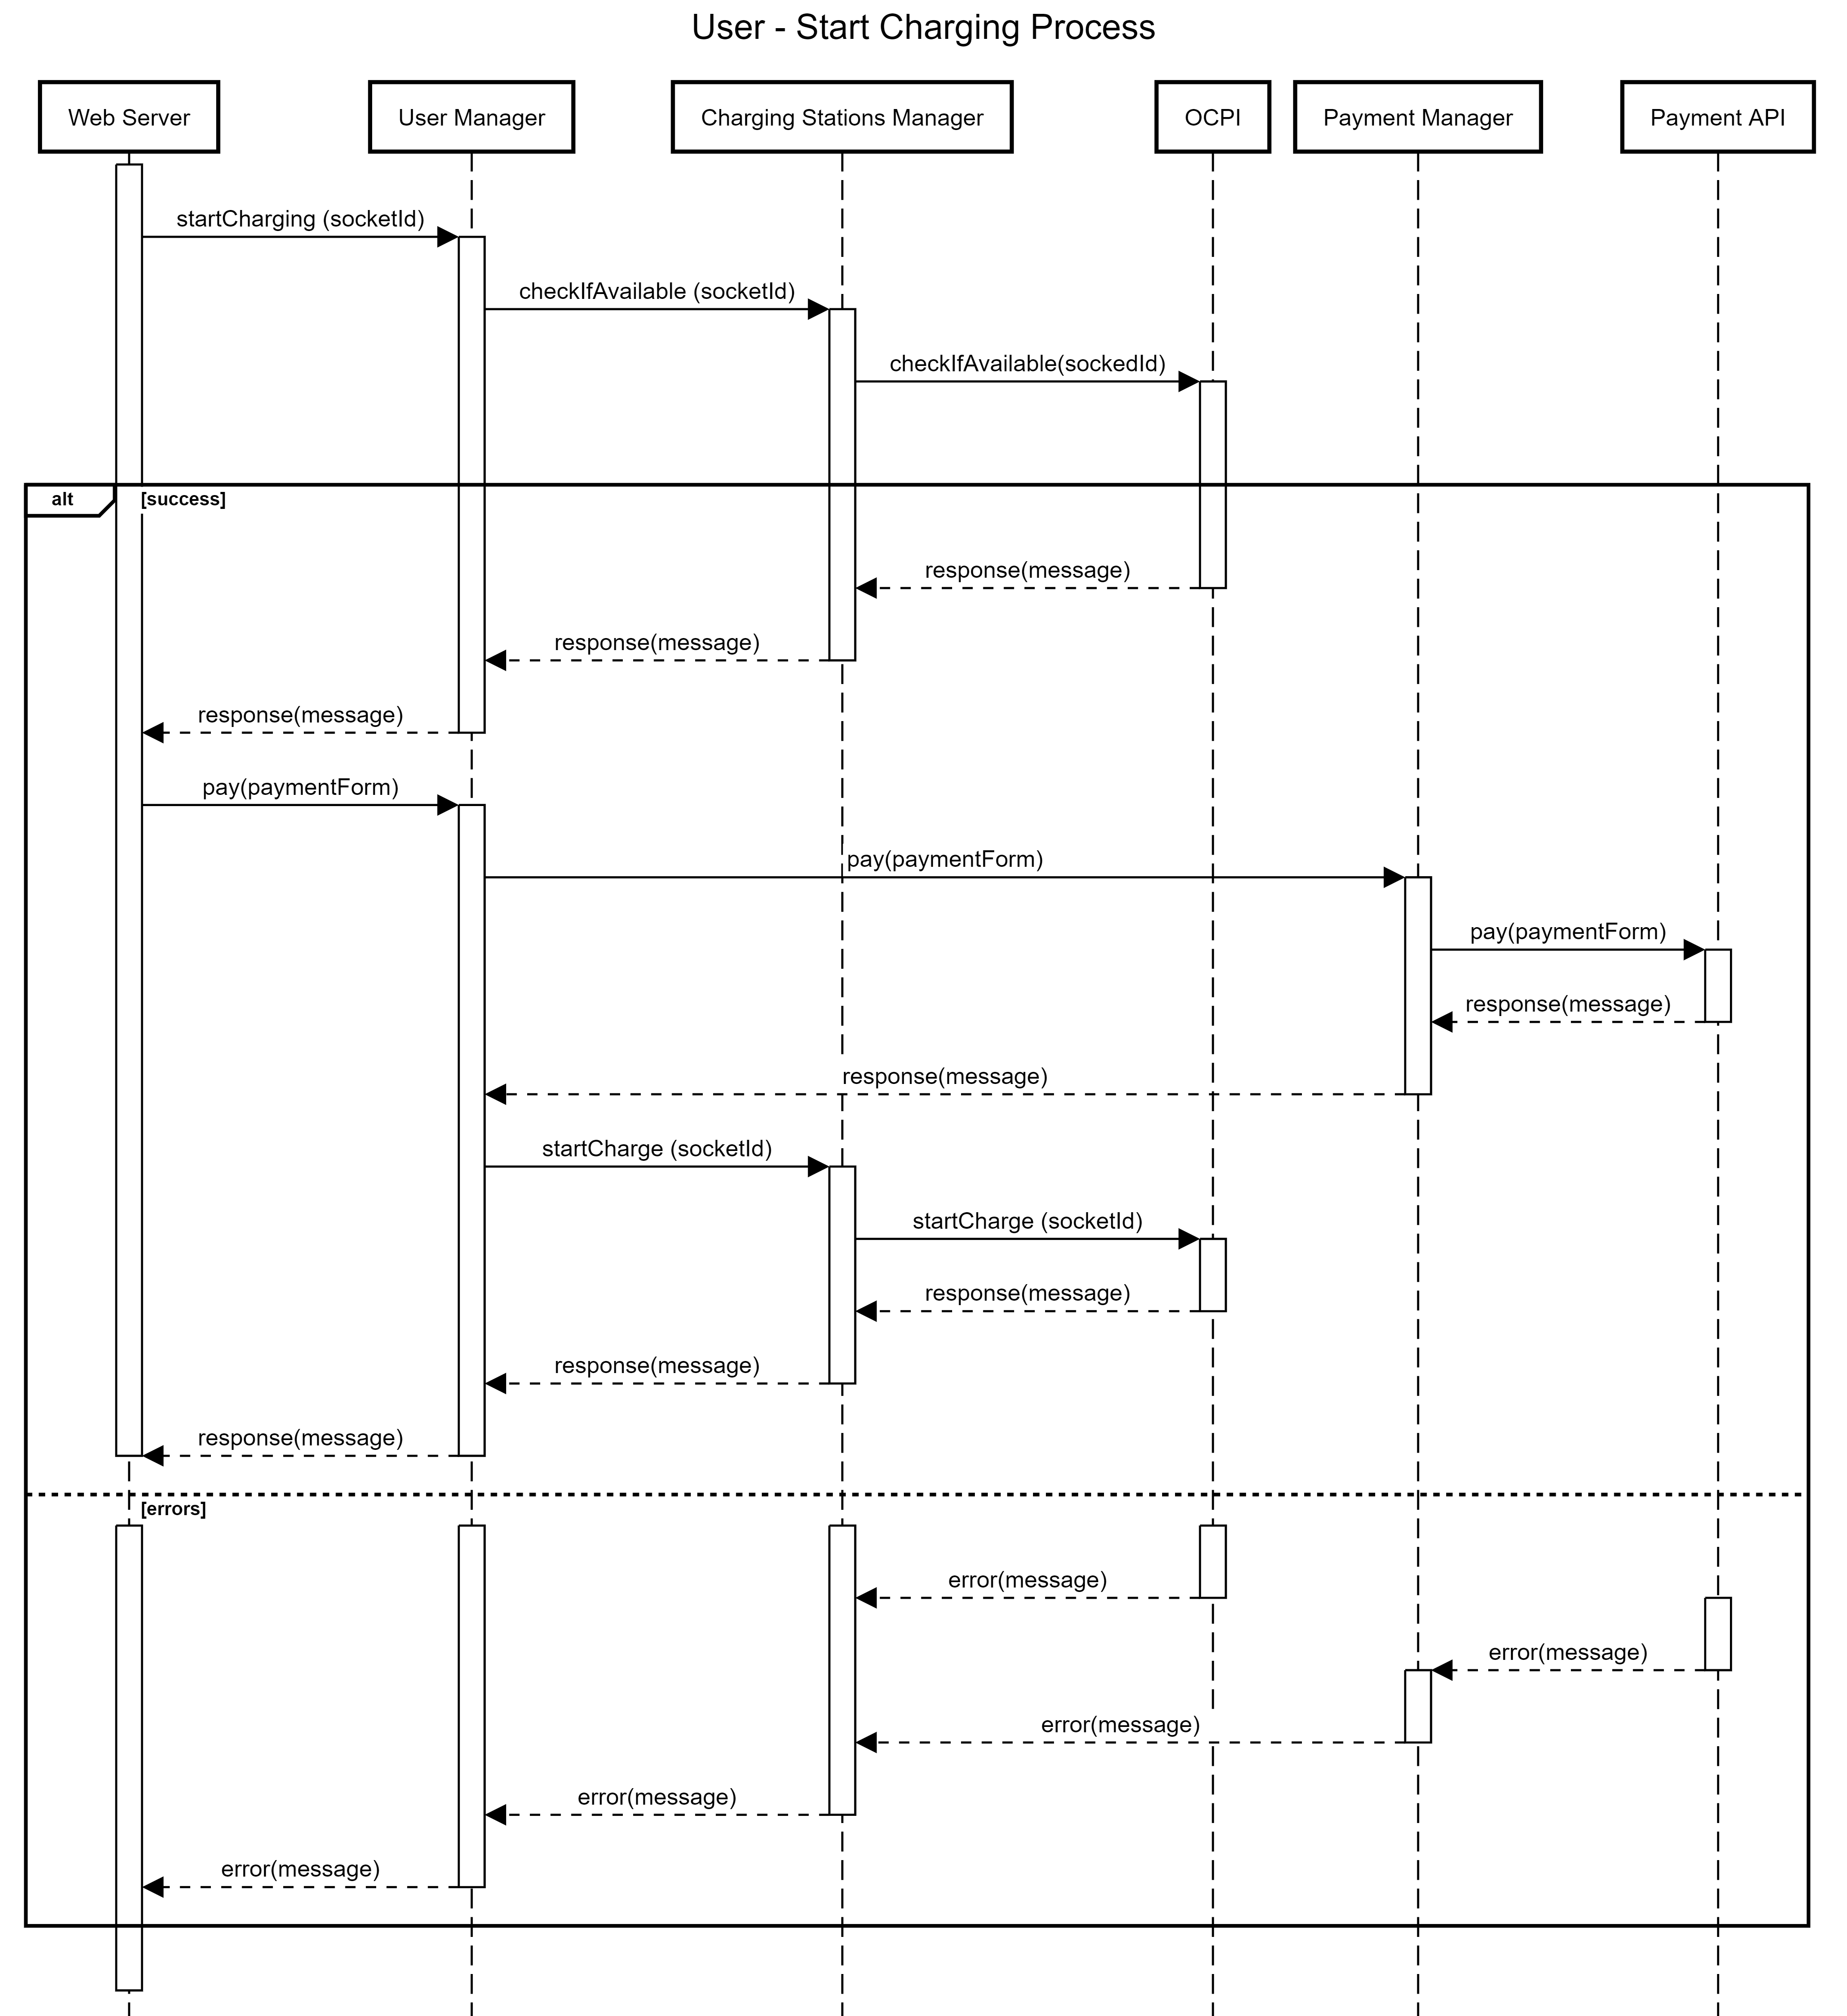
\includegraphics[scale=0.10, center]{assets/sequenceDiagrams/User Start Charging Process.png}
        \caption{Start Charging Process}
        \label{Start Charging Process}
    \end{figure}
\end{center}
This sequence explains what happens after a User plugs his EV to a charging point and presses "Start charging" on the button of the respective socket. For the sake of readability, throughout the first part of the alt it is assumed all interactions end with success. Errors will be explained later.\newline
Firstly a socketID is sent to the Charging Stations Manager, to check whether the requested socket is available as it could be booked or unavailable. If the request is positive, the user is shown
a form for the payment that will be compiled and sent back to the Payment Manager. The Payment Manager will proceed to send the information to the Payment API that will actuate the actual payment.
When the payment goes through, the User Manager will communicate to the OCPI through the Charging Stations Manager that the charge can start. The OCPI will then send data regarding the status back to the User.
The errors will be now explained more thorougly. \newline Firstly, an error could be raised by the OCPI in case the requested socket is not currently available.
Secondly, an error could be caused by the Payment Manager in the case the payment Form contains invalid data. The third error could be raised by the Payment API in case the payment process doesn't end successfully.
It is important to note that we assume that once the user has payed the OCPI cannot fail in starting the charge, as its availability was checked beforehand. If this wasn't the case, there could be instances where the User pays and the charge doesn't actually start.

\newpage
\textbf{Schedule suggestions}
\begin{center}
    \begin{figure}[H]
        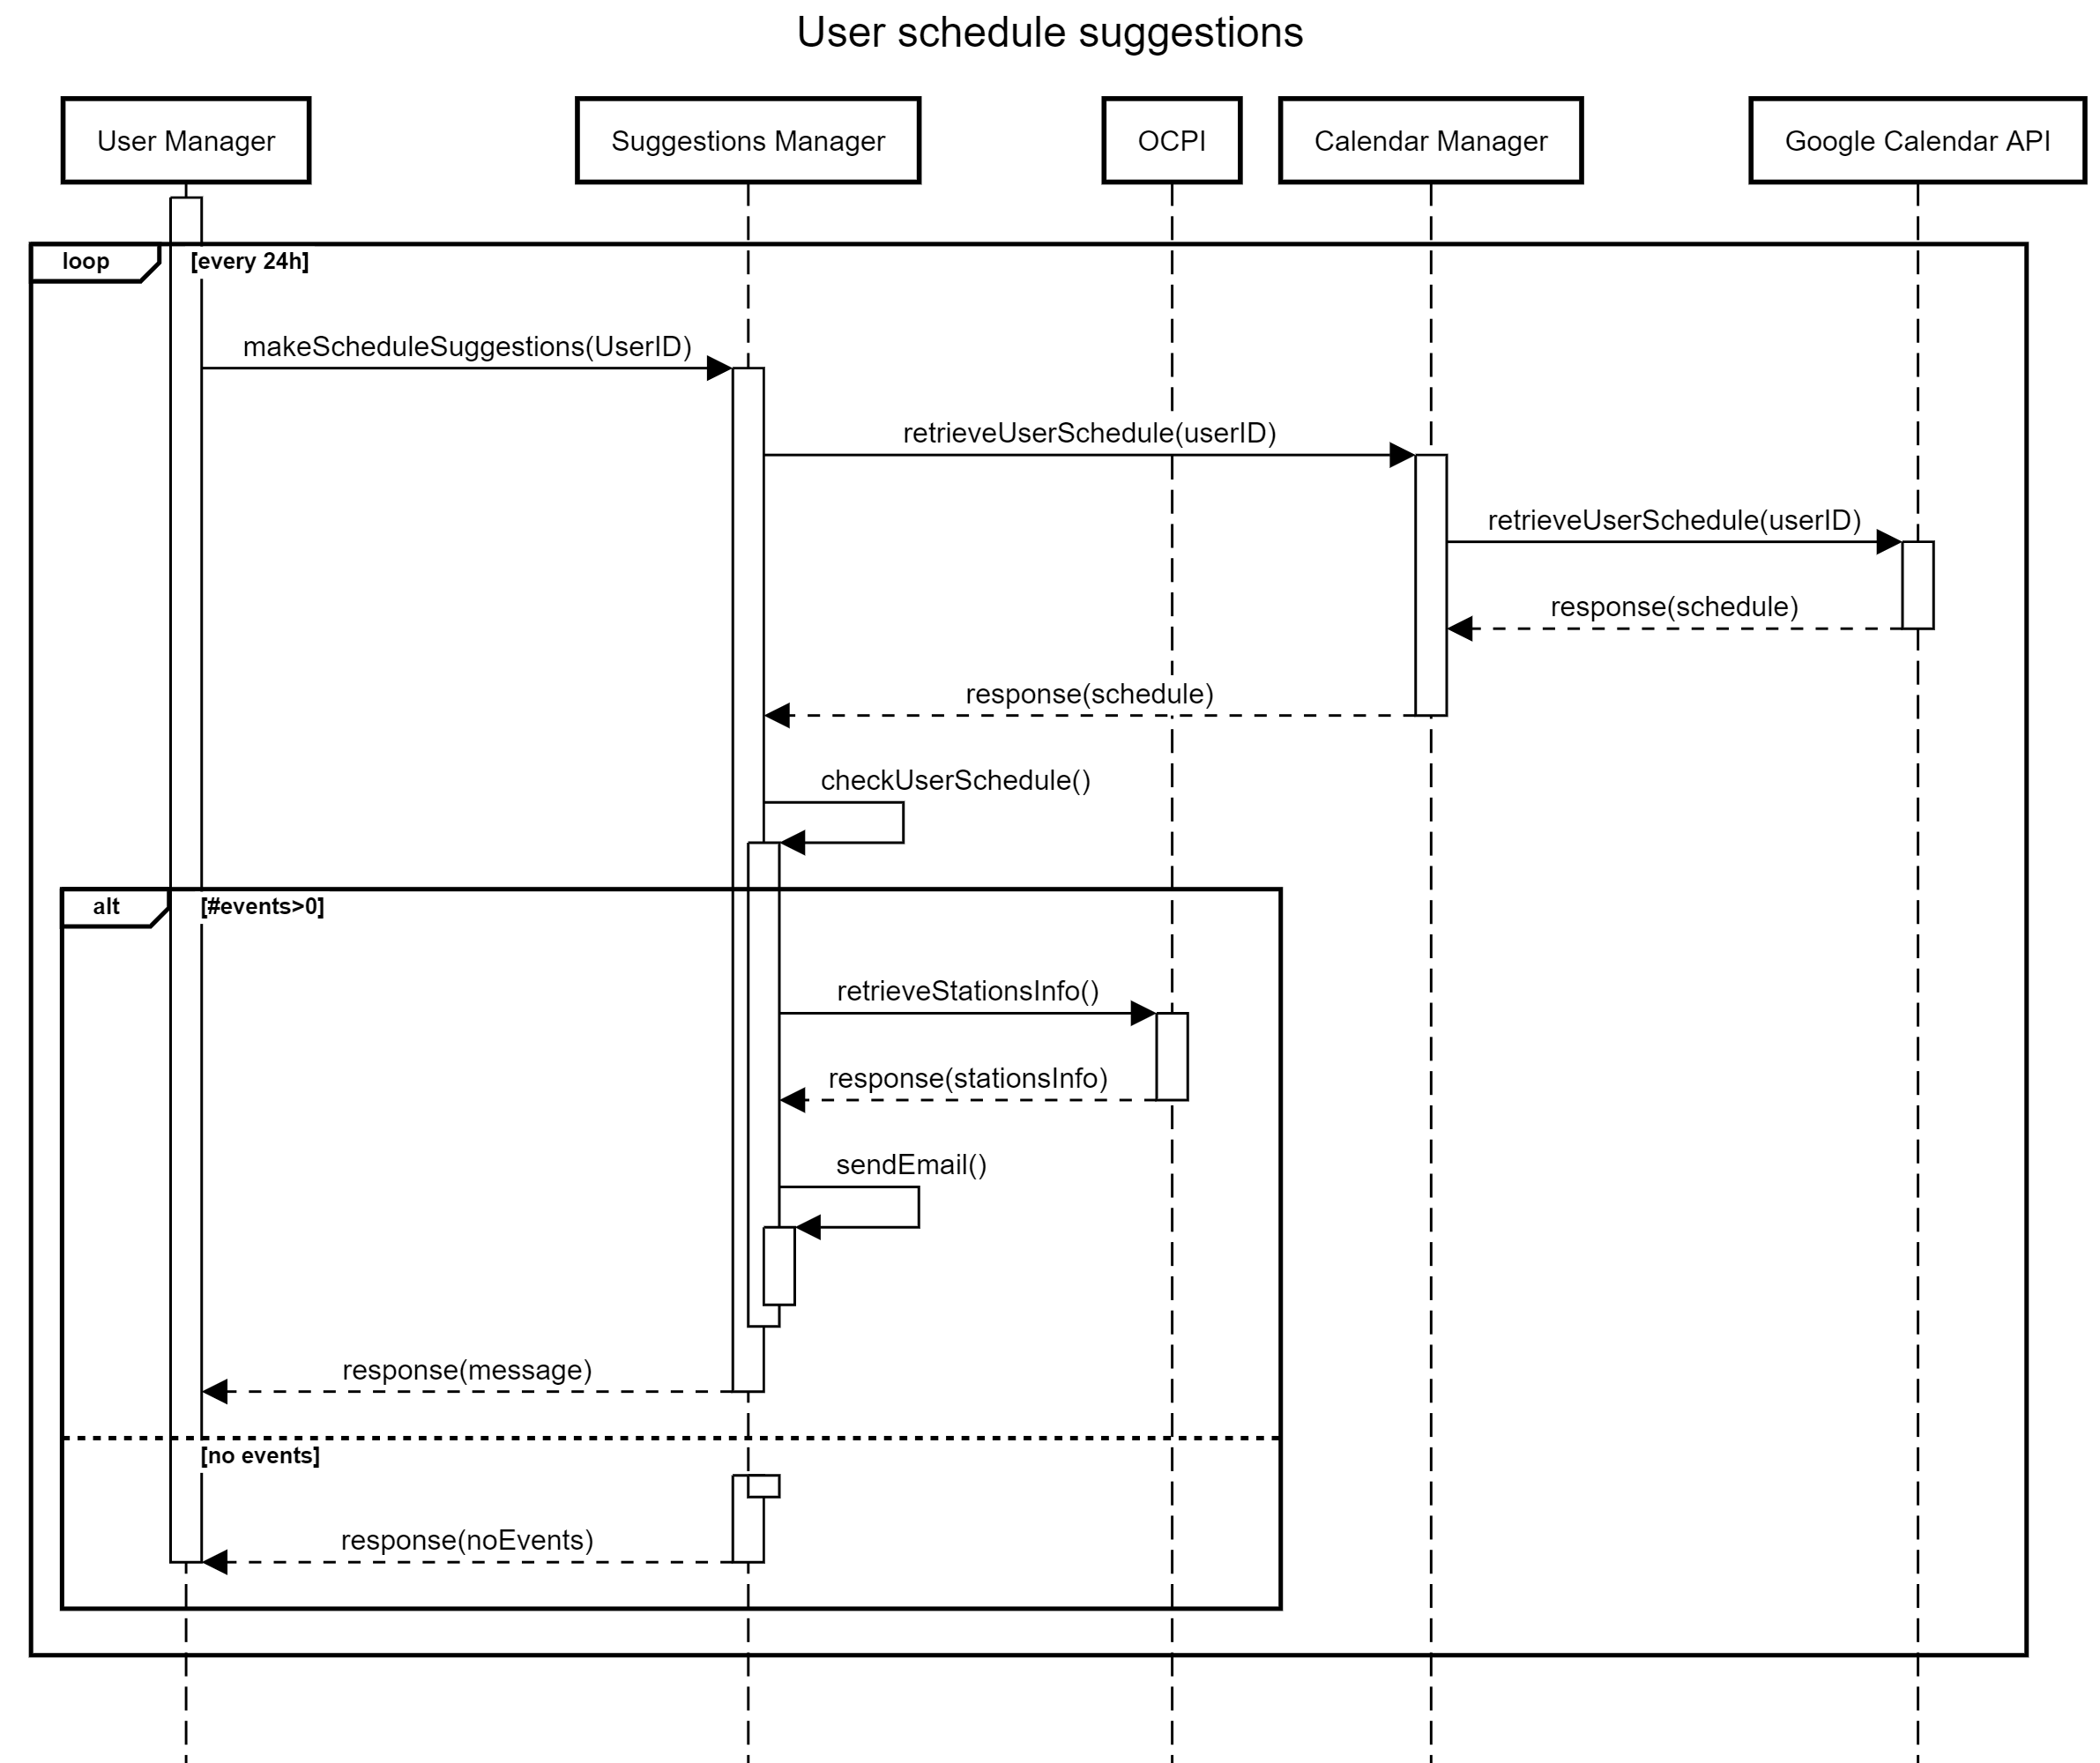
\includegraphics[scale=0.20, center]{assets/sequenceDiagrams/User schedule suggestions.png}
        \caption{Schedule suggestions}
        \label{Schedule suggestions}
    \end{figure}
\end{center}
\newpage
The user's schedule suggestion service triggers a check every day at 00:00 to see if the user has planned some events for the next day.
When it triggers, the SuggestionManager calls the CalendarManager in order to retrieve the user's schedule for the next day by using the Google Calendar API.
Then the SuggestionManager checks all the new events: if there is at least one event it retrieves a list of charging stations information that are nearby the event's location by communicating with the OCPI component, and then sends an eMail with a list of charging stations based on their distance, cost and special offers.
The email will contain a link for each station that will redirect the user to a pre-filled booking form, in order to easily book a socket.
\newpage

\textbf{Battery suggestion}
\begin{center}
    \begin{figure}[H]
        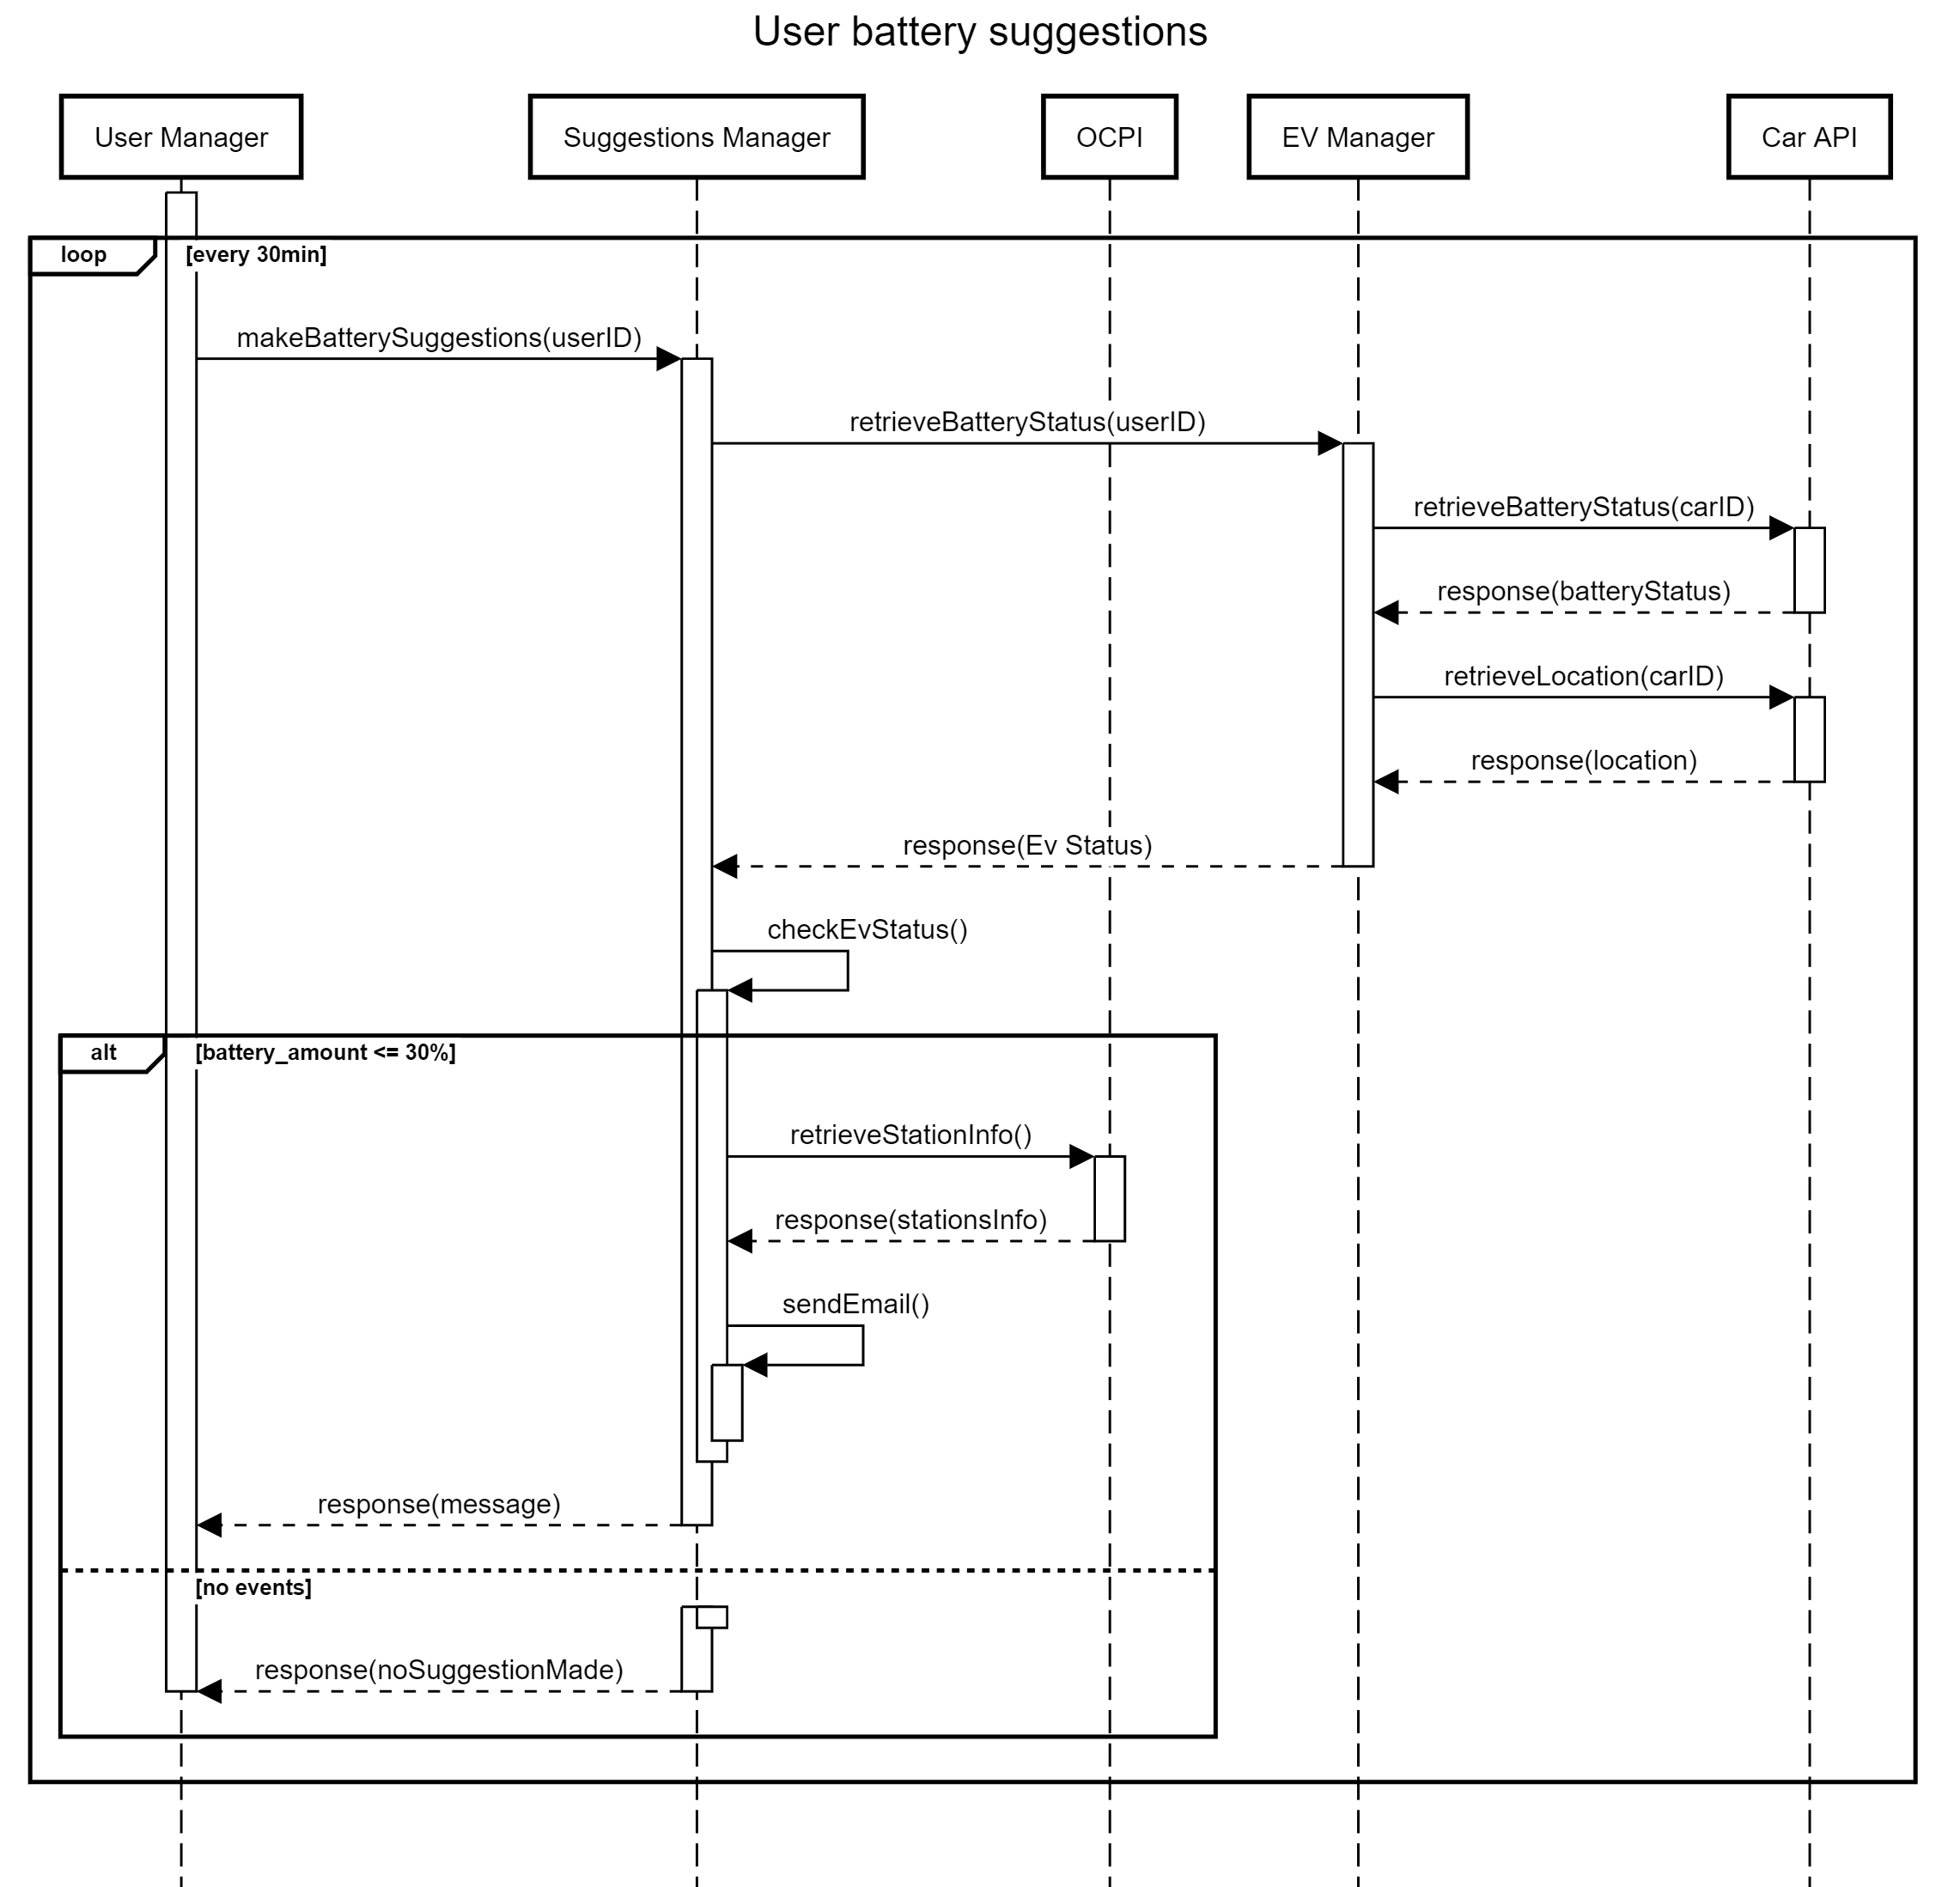
\includegraphics[scale=0.20, center]{assets/sequenceDiagrams/battery suggestions.png}
        \caption{Battery suggestion}
        \label{Battery suggestion}
    \end{figure}
\end{center}
\newpage
The battery suggestion service triggers a check every 30 minutes to see if the user'EV has battery status below a certain threshold.
When it triggers, the SuggestionManager calls the EVManager in order to retrieve the user's car battery status and location by using the CarAPI.
Then the SuggestionManager checks the battery status: if it's below a certain threshold it retrieves a list of charging stations information that are nearby the user's home or the car location by communicating with the OCPI component, and then sends an eMail with a list of charging stations based on their distance, cost and special offers.
Note that this service is available only for the users that have a car registered in the system and that have a brand that supports this features with their API.
\newpage

\underline{\textbf{CPOW diagrams}}\\
\textbf{Insert discount}
\begin{center}
    \begin{figure}[H]
        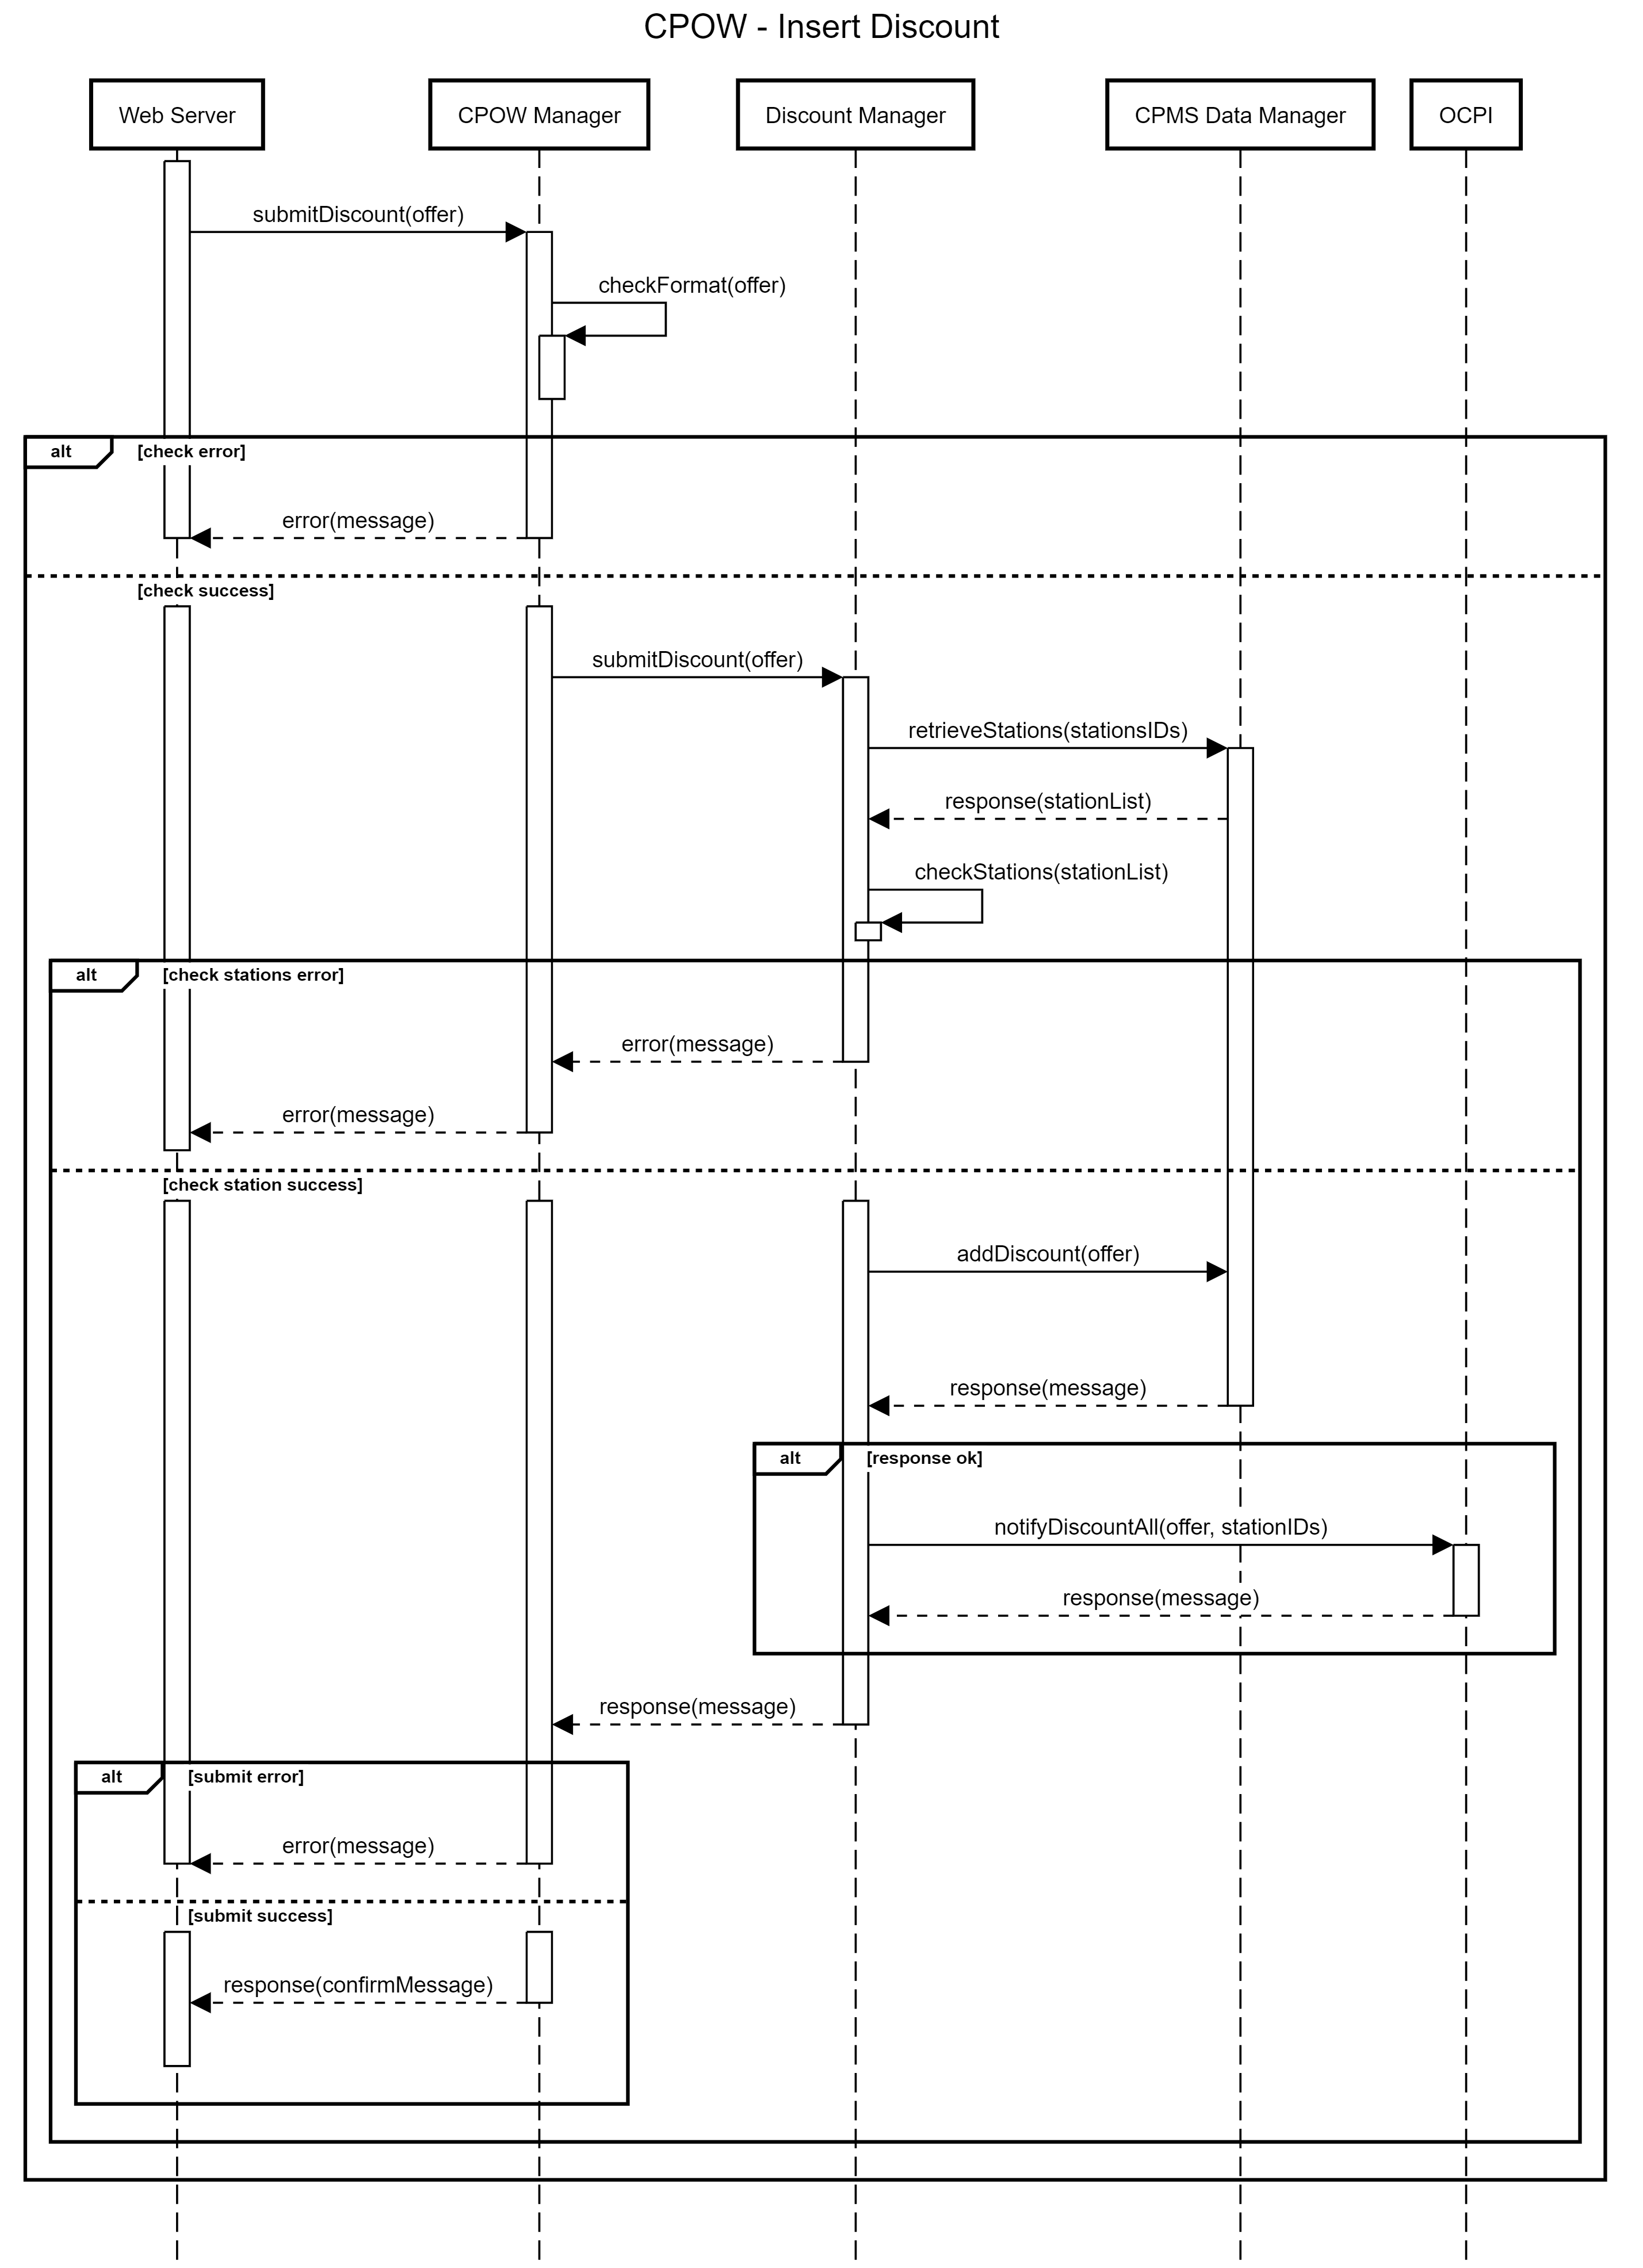
\includegraphics[scale=0.12, center]{assets/sequenceDiagrams/CPOW insert discount.png}
        \caption{CPOW - Insert discount}
        \label{CPOW - Insert discount}
    \end{figure}
\end{center}
The insert discount interaction triggers when a CPOW wants to insert a new discount for a list of charging stations.
After receiving the form information, the CPOW Manager calls the Discount Manager in order to check if the stations are valid and if the discount is valid.
Then the discount is inserted in the database and the Discount Manager calls the OCPI component in order to notify all EMSPs that are connected to the CPMS about the new discount.
Note that in this diagram it is not showed the interaction with the OCPP component because it will apply the discount to the charging stations only when the discount's start date is reached.
\newpage

\textbf{Delete discount}
\begin{center}
    \begin{figure}[H]
        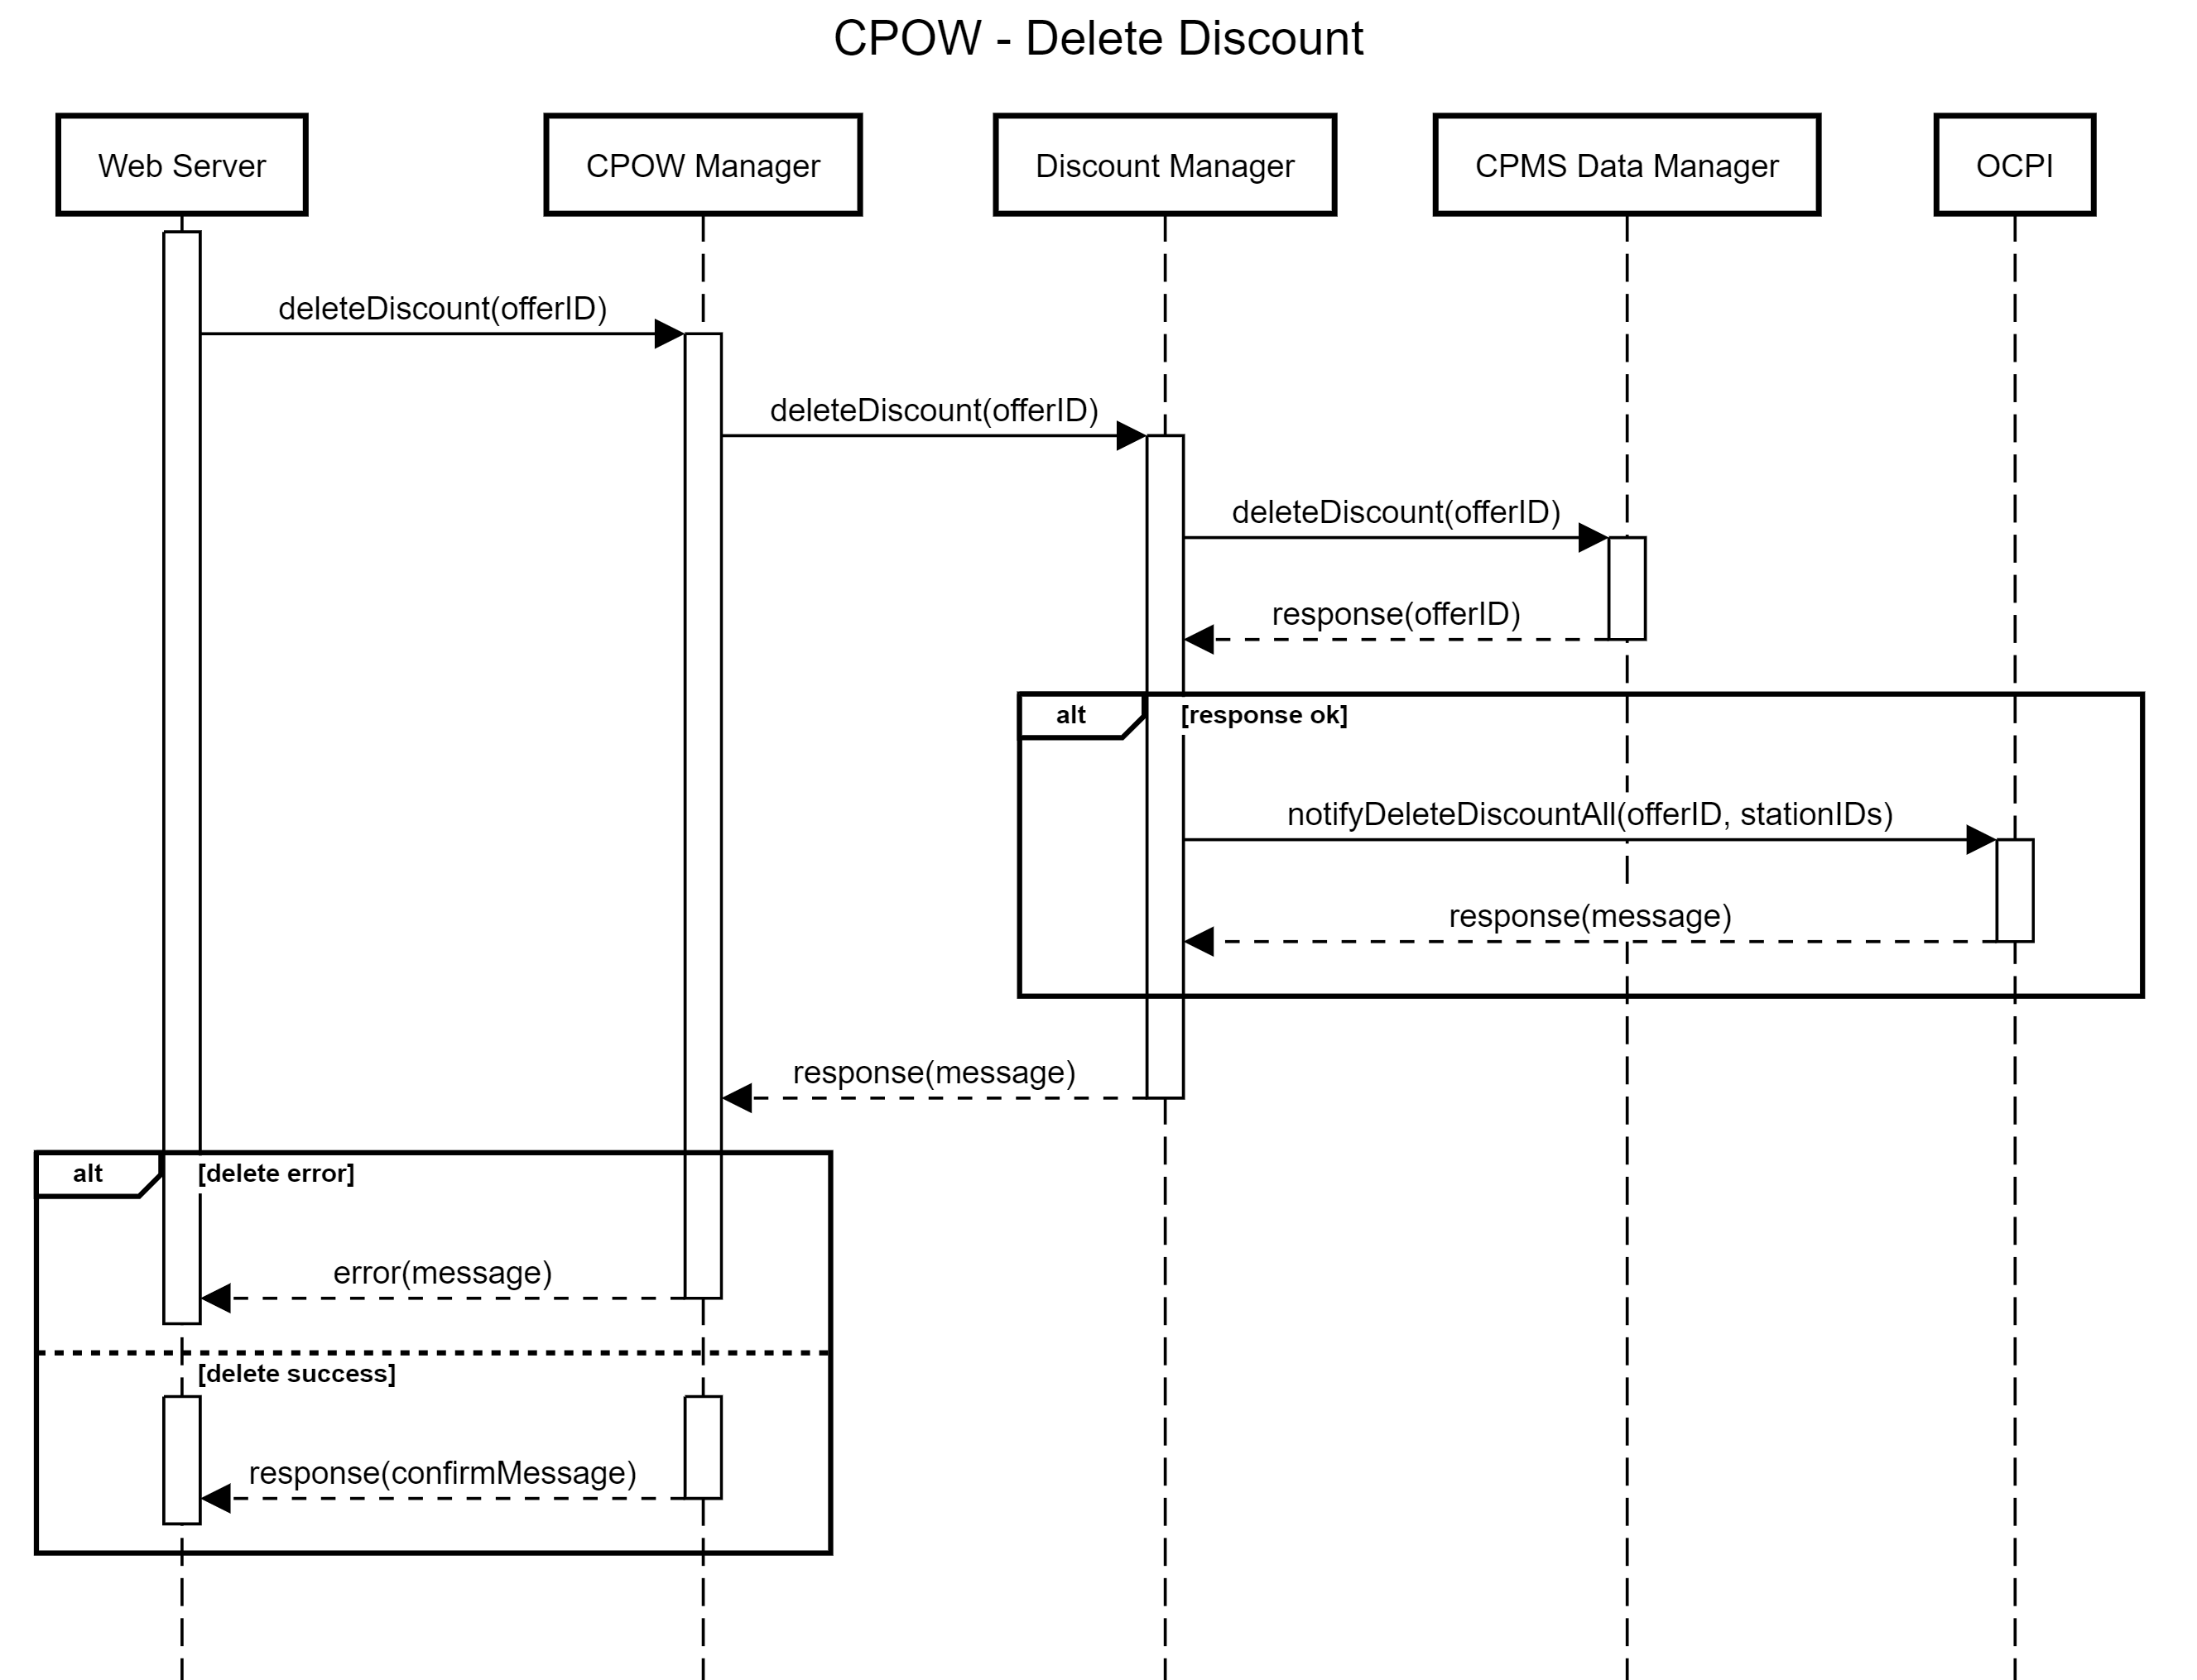
\includegraphics[scale=0.15, center]{assets/sequenceDiagrams/CPOW delete discount.png}
        \caption{CPOW - Delete discount}
        \label{CPOW - Delete discount}
    \end{figure}
\end{center}
The delete discount interaction triggers when a CPOW wants to delete a discount for all the charging stations to which it was applied.
After receiving the discountID, the system will check if the discount exists. If it is, it will delete it from the database and notify all EMSPs that are connected to the CPMS.
\newpage

\textbf{View charging stations}
\begin{center}
    \begin{figure}[H]
        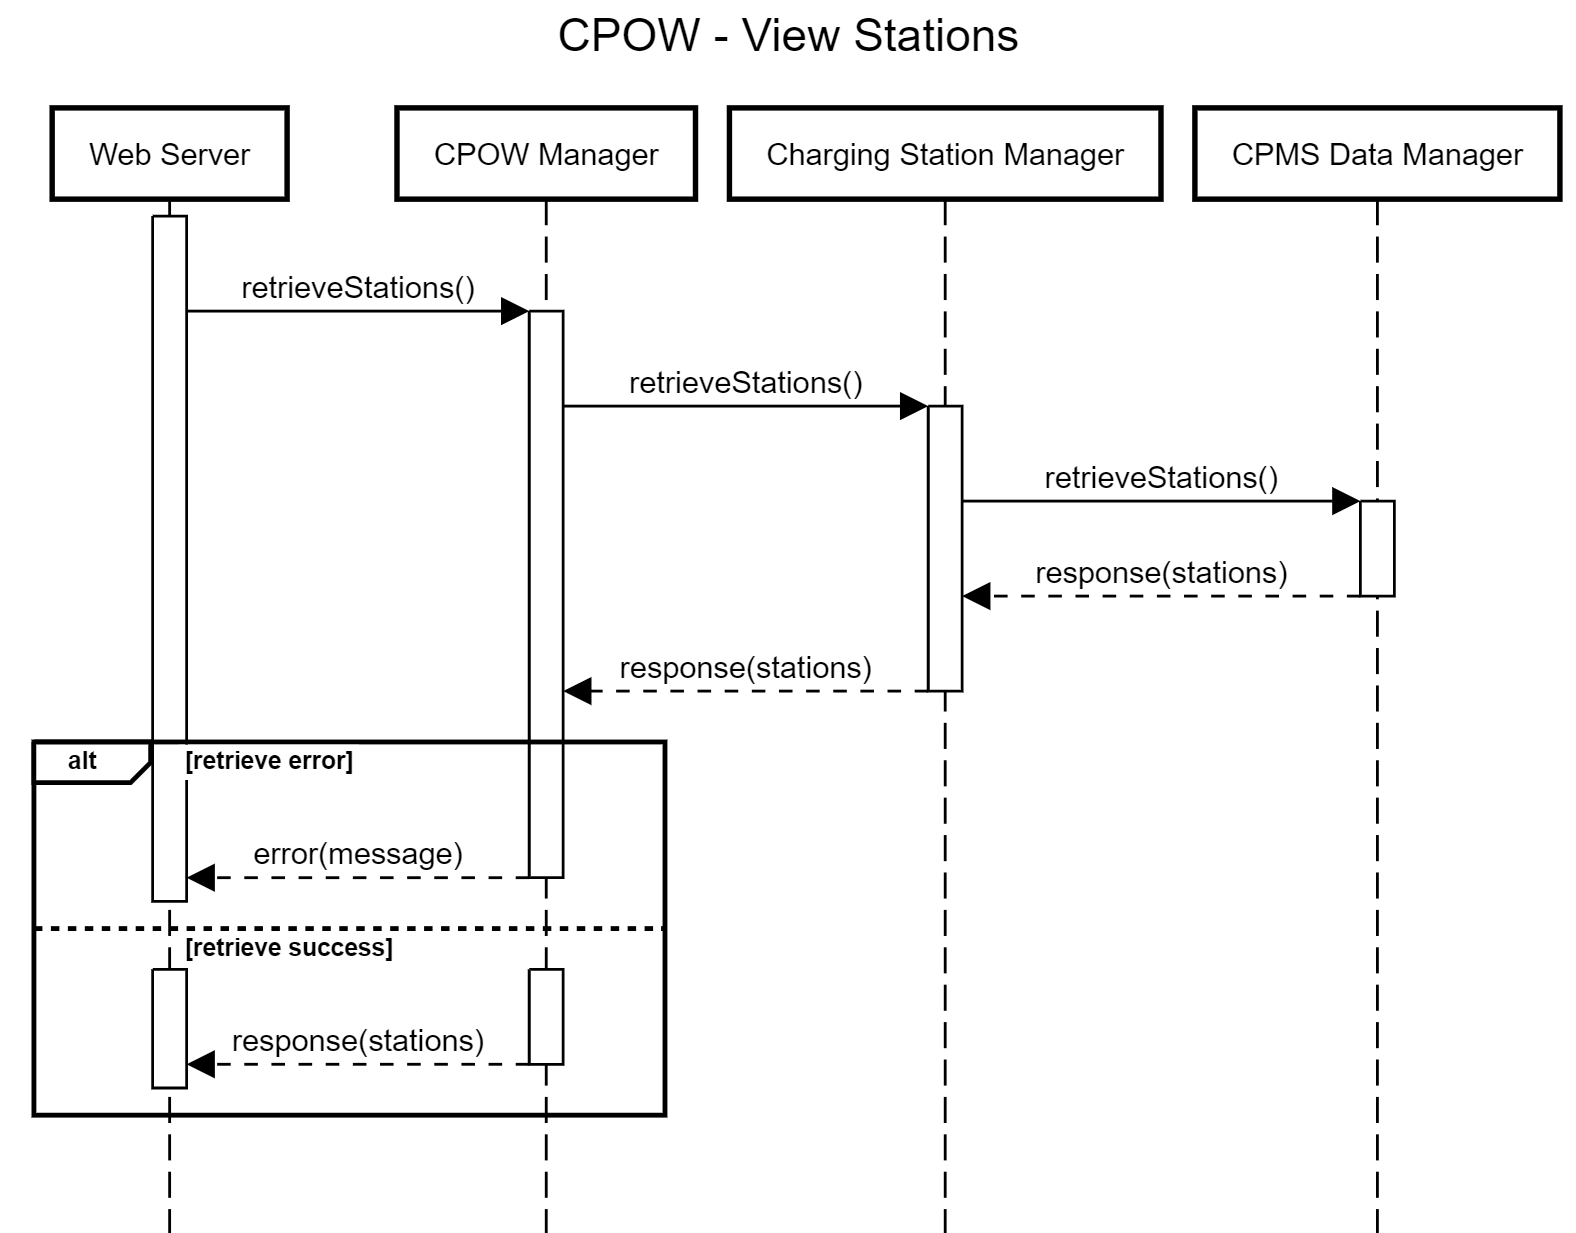
\includegraphics[scale=0.25, center]{assets/sequenceDiagrams/CPOW view stations.png}
        \caption{CPOW - View charging stations}
        \label{CPOW - View charging stations}
    \end{figure}
\end{center}
This diagram describes the data fetching interaction between the Web Server and the Applicantion Server in order to retrieve the list of charging stations that are connected to the CPMS.
The list will contain all the stations details, such as the ID, the location, the energy provider, the status and the socket details and a button to change the energy provider.
\newpage

\textbf{Change energy provider}
\begin{center}
    \begin{figure}[H]
        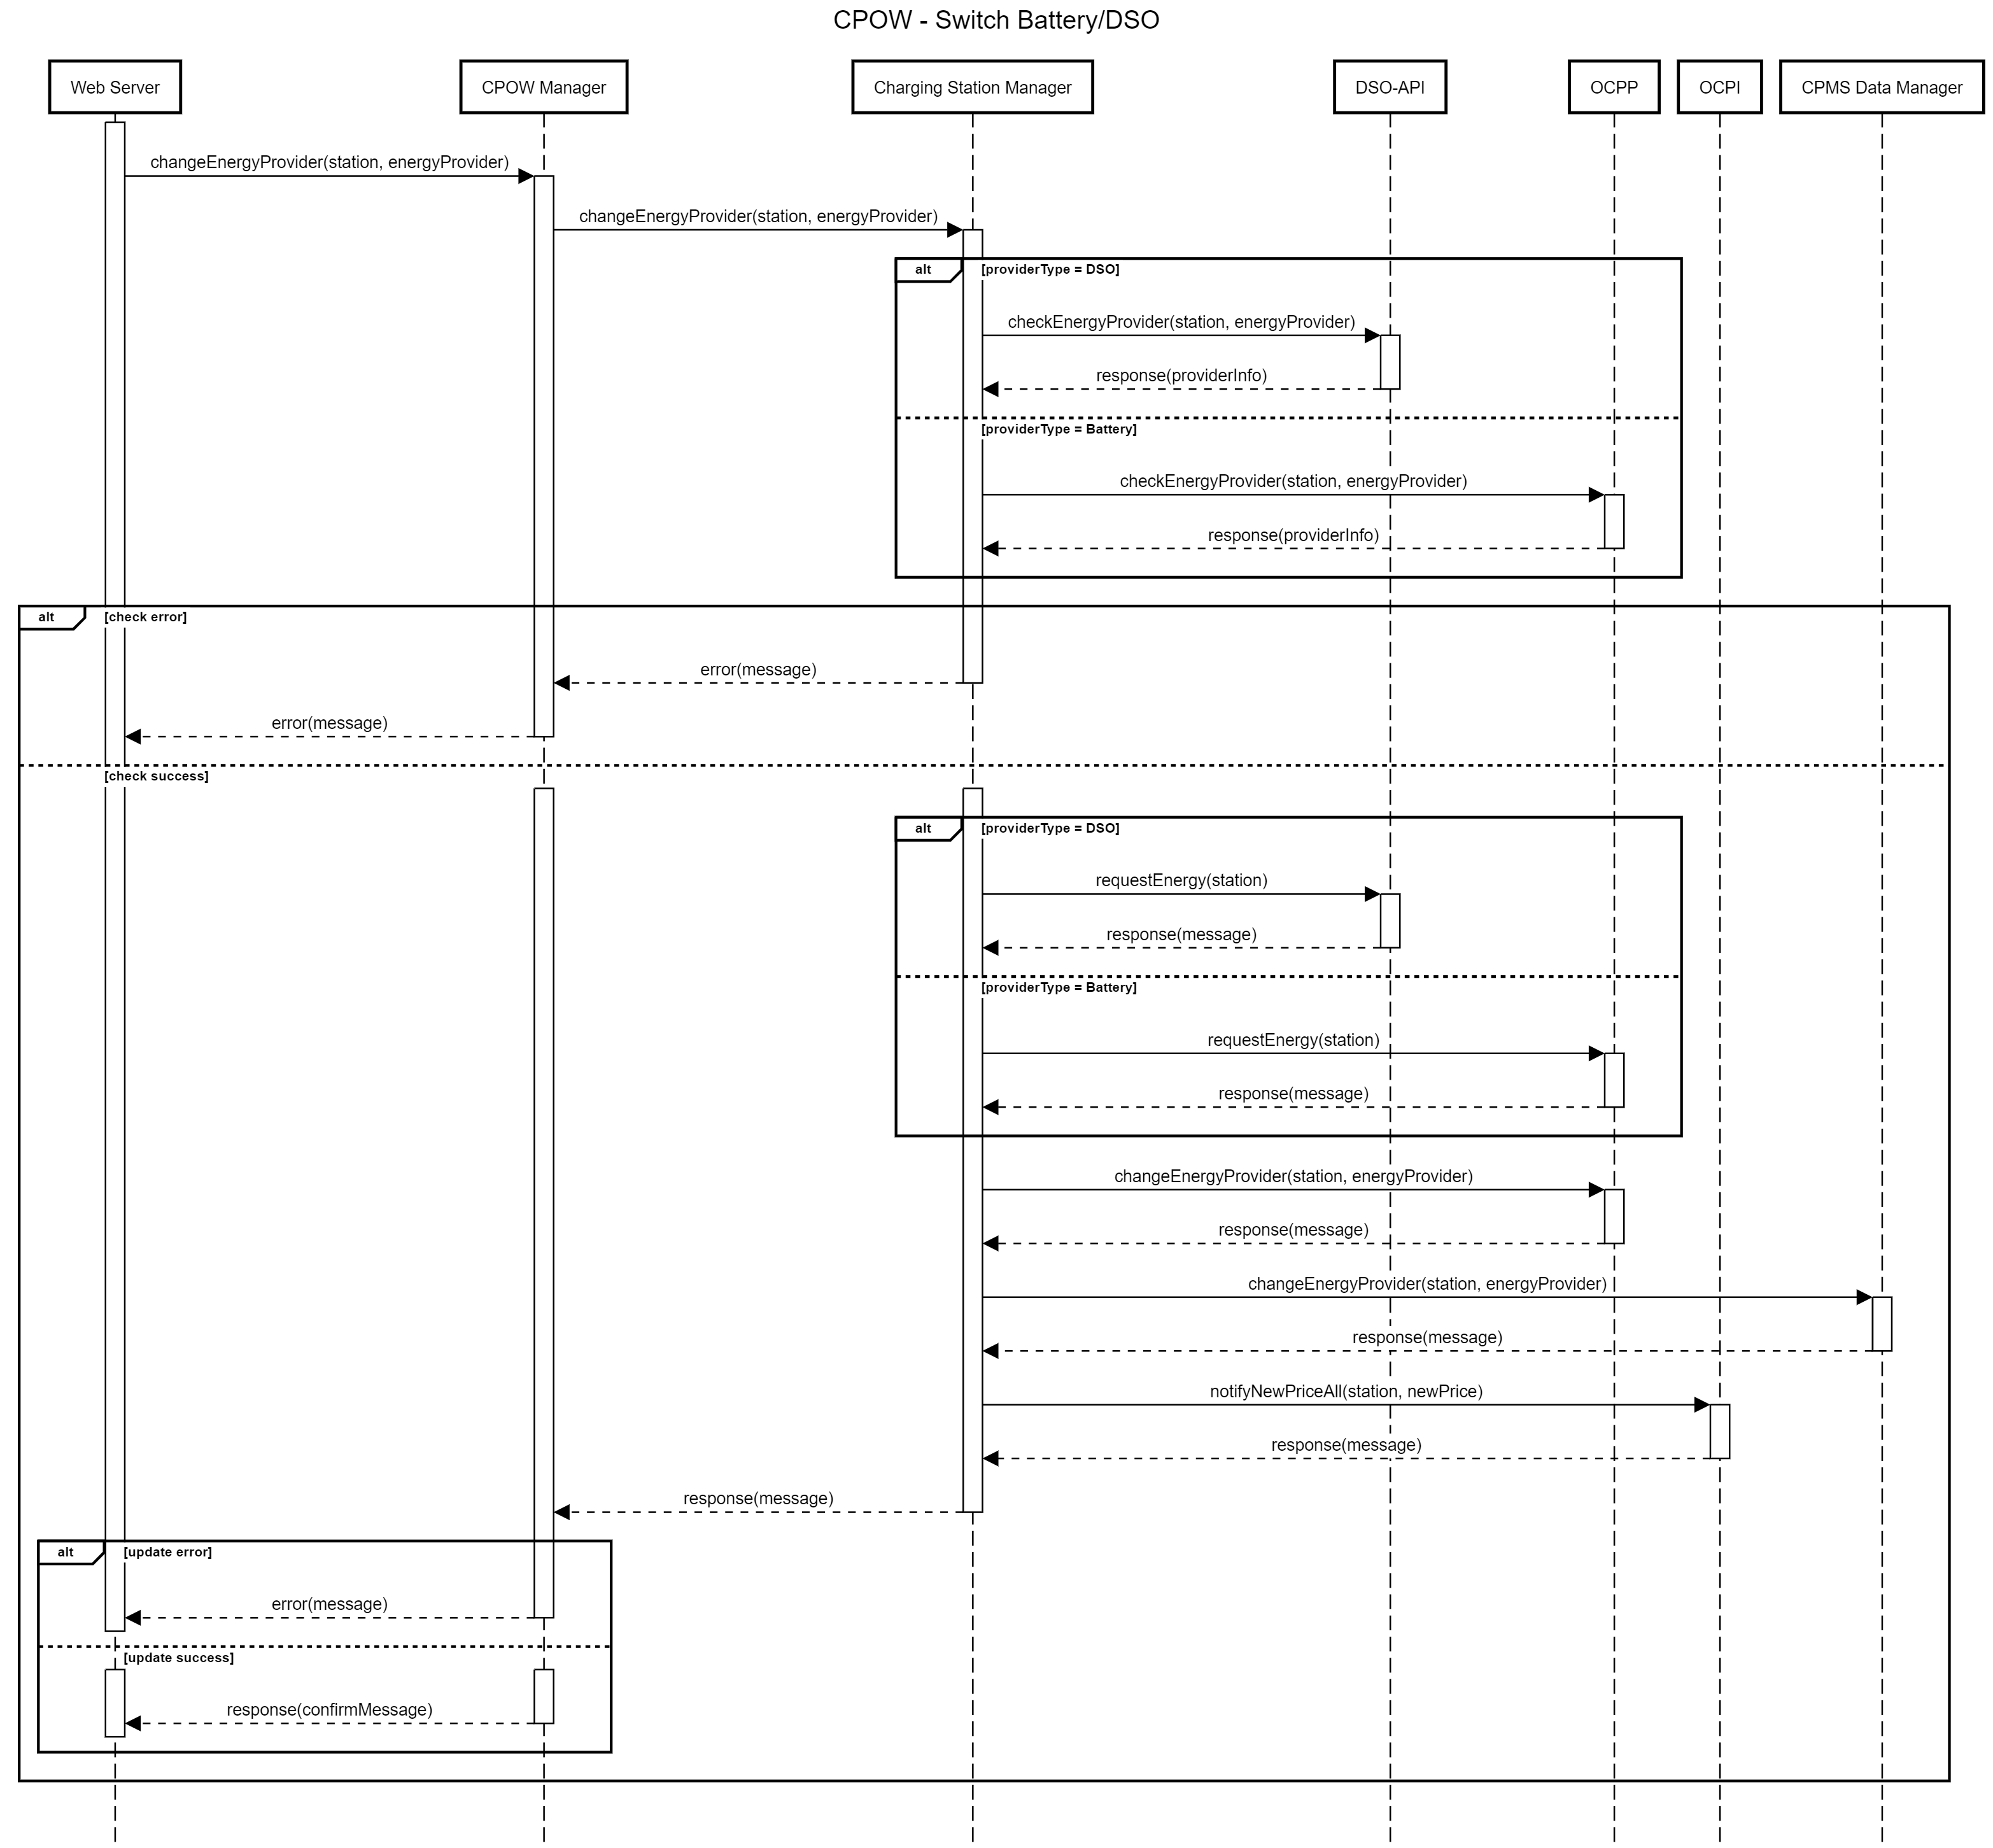
\includegraphics[scale=0.15, center]{assets/sequenceDiagrams/CPOW change energy.png}
        \caption{CPOW - Change energy provider}
        \label{CPOW - Change energy provider}
    \end{figure}
\end{center}
\newpage
This diagram describes the interaction between the CPOW and the Applicantion Server in order to change the energy provider of a charging station.\\
It starts by the CPOW sending a request with the charging station ID and the new energy provider (after retrieving a list with all the stations details, described in Figure \ref*{CPOW - View charging stations}).
Then, the Charging Station Manager will check if the station exists and if the energy provider is valid by communicating with the OCPP or the DSO-API component, depending if the selected provider is a DSO or an internal battery.
If the selected provider is available, the Charging Station Manager will ask the Provider to start supplying the energy, notify the station through OCPP, notify the connected eMSPs through OCPI, and update the station's current energy provider in the database.
\newpage


\subsection{Component interfaces}
\underline{\textbf{eMSP}}\\
\begin{center}
    \begin{figure}[H]
        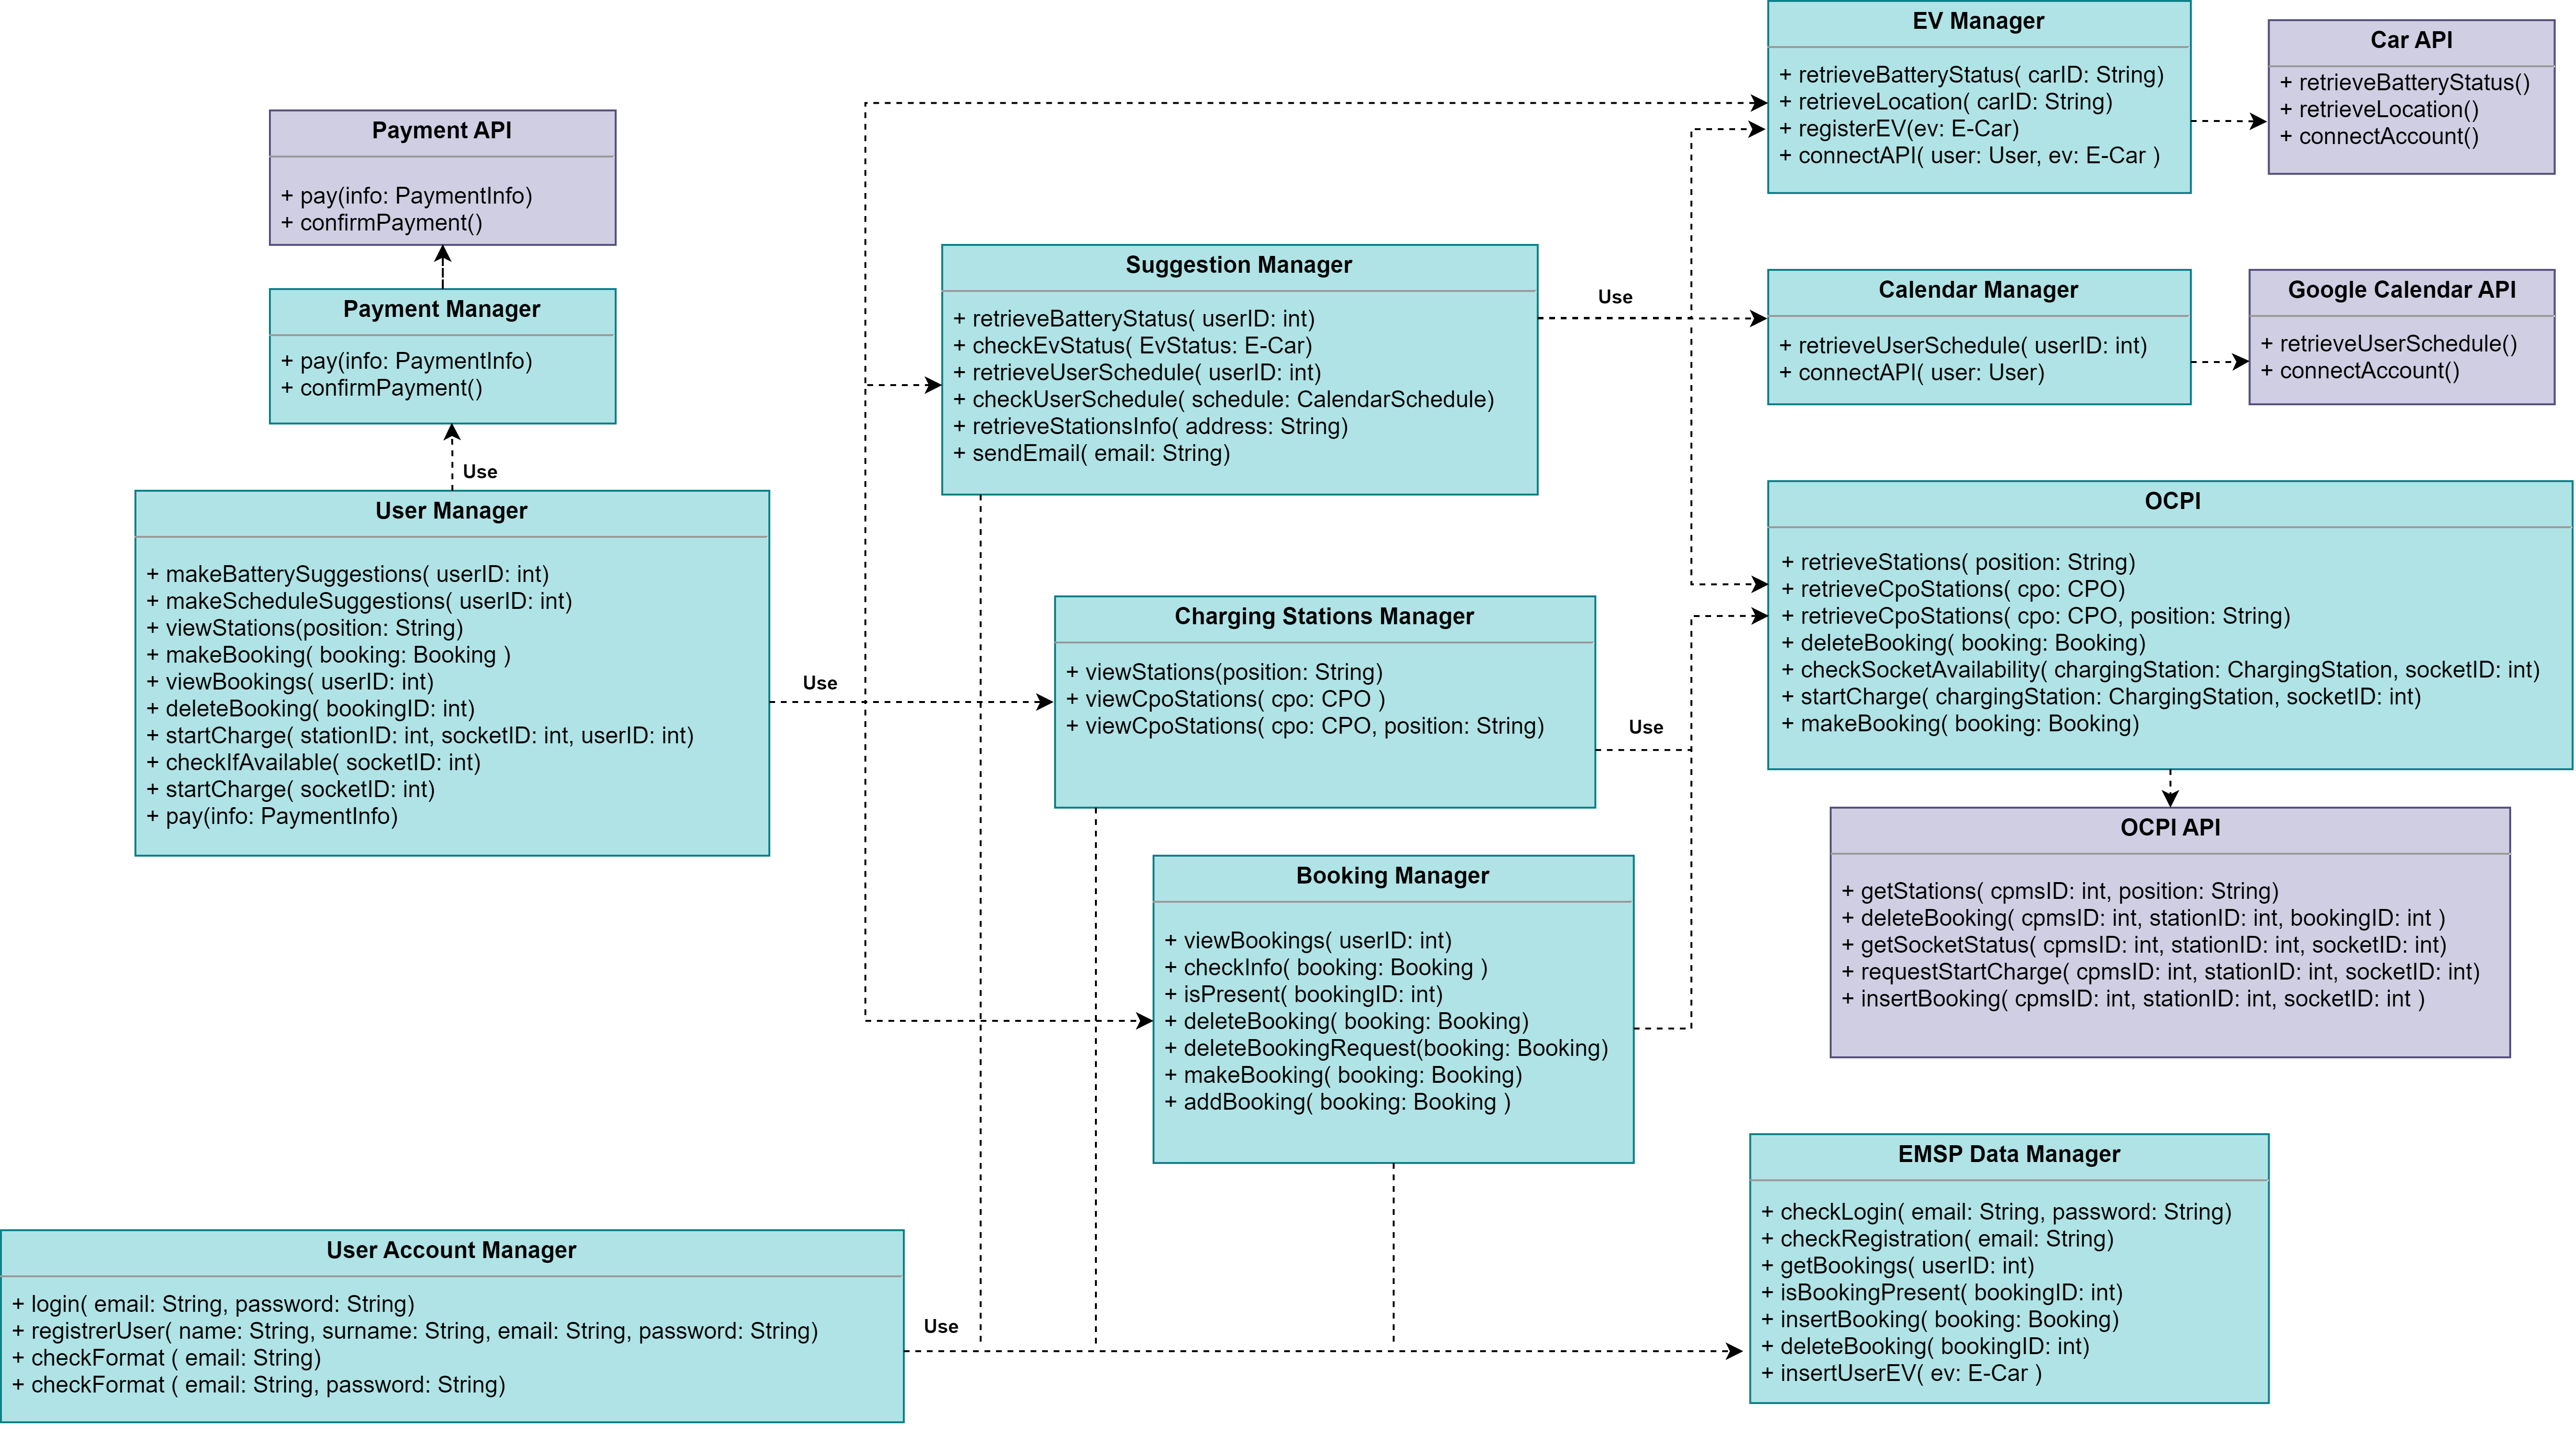
\includegraphics[scale=0.59, center]{assets/interfacesDiagrams/EMSP interface diagram.png}
        \caption{EMSP Component Interfaces Diagram}
        \label{fig: EMSP component_interfaces}
    \end{figure}
\end{center}

This diagram above describes in detail the interfaces and the corresponding methods offered by each component of the eMSP, it also shows the interaction between them as described in Fig. \ref*{fig: application_server_component_view}.\\
Please note that the described methods do not represent exactly the final version that will be used during the implementation, they just provide a logical representation.
\newpage

\underline{\textbf{CPMS}}\\
\begin{center}
    \begin{figure}[H]
        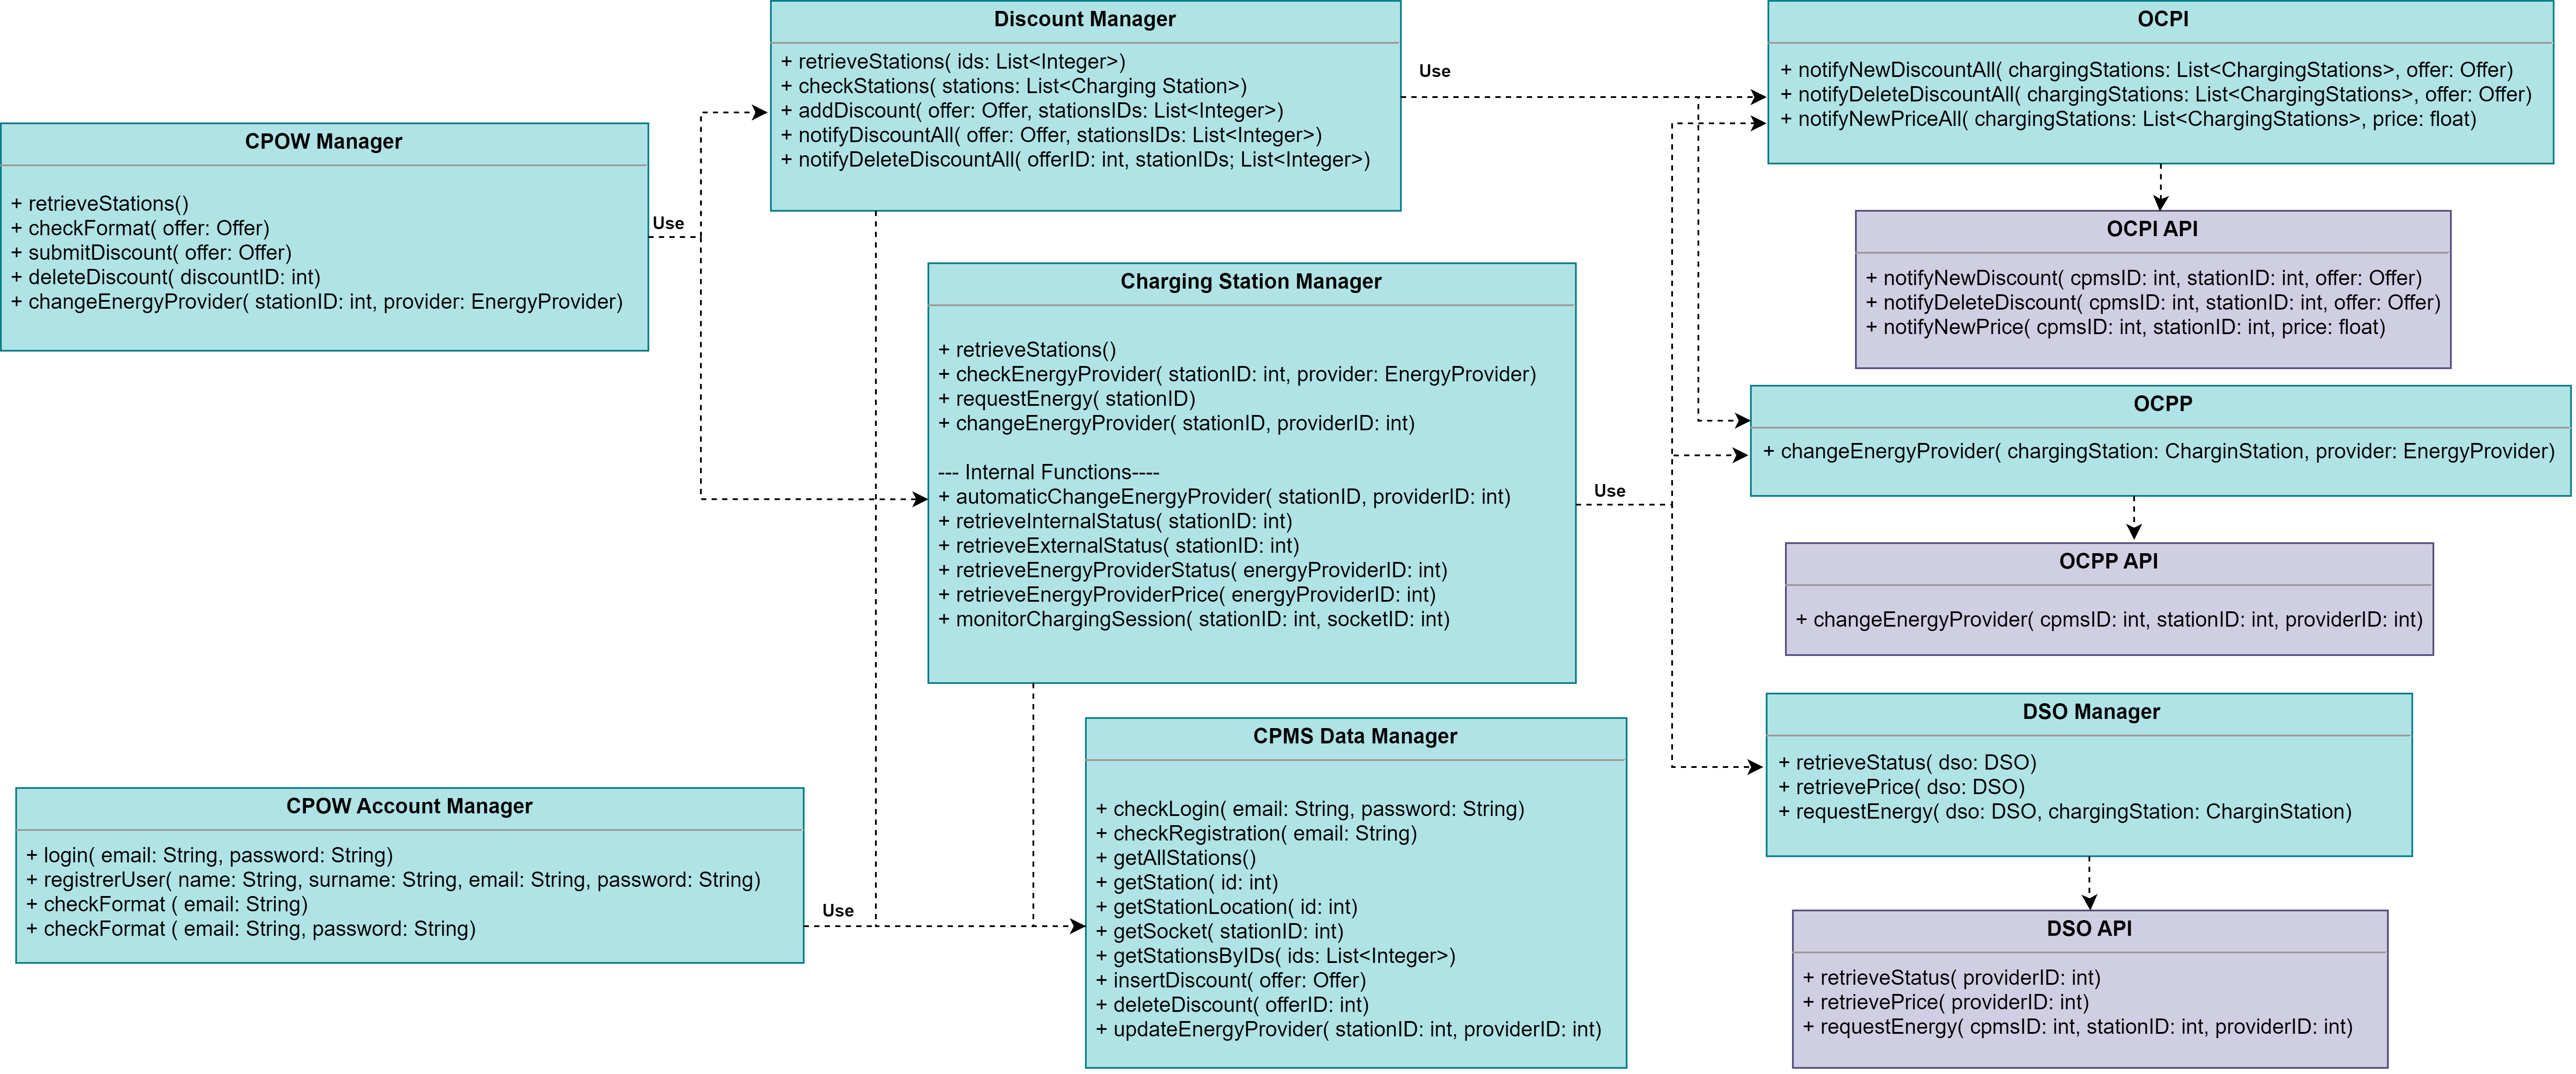
\includegraphics[scale=0.55, center]{assets/interfacesDiagrams/CPMS interface diagram.png}
        \caption{CPMS Component Interfaces Diagram}
        \label{fig: CPMS component_interfaces}
    \end{figure}
\end{center}

This diagram above describes in detail the interfaces and the corresponding methods offered by each component of the CPMS, it also shows the interaction between them as described in Fig. \ref*{fig: application_server_component_view}.\\
Please note that the described methods do not represent exactly the final version that will be used during the implementation, they just provide a logical representation.
\newpage

\subsection{Selected architectural styles and patterns}

    \begin{itemize}
        \item \textbf{Three tier architecture} \newline
        The selected architecture for this system is a three tier architecture, which consists of a presentation tier, a logic tier, and a data tier. The presentation tier is responsible for displaying information to the user and accepting input, the logic tier is responsible for processing the input and performing any necessary calculations or operations and lastly the data tier is responsible for storing and retrieving data from a database.
        \item \textbf{Thin client} \newline
              The thin client approach increases security, since sensitive data will not be stored locally, and scalability, because it allows for an easier deployment of new clients, while also granting a more centralized management.
        \item \textbf{Scalability} \newline
              A three tier architecture allows for a more modular design, meaning that it's easier to scale individual components of the system as changes to one component do not necessarily require changes to the other components.
        \item \textbf{Model View Controller} \newline
        The Model-View-Controller (MVC) design pattern is a software design pattern that separates an application into three main components: the model, the view, and the controller. The model represents the data and business logic of the application, the view represents the user interface, and the controller mediates communication between the model and the view. In particular:
              \begin{itemize}
                  \item Model: The central component of the pattern, it's the dynamic data stracture of the application, meaning that it changes as data is added modified and deleted, it's indipendent of the user interface as it's not concerned with how the data is displayed and how the user interacts with the application and it directly manages the data, logic, and rules of the application.
                  \item View: It represents the user interface of the application. It responsible for displaying information and accepting imput from the user. It defines how the application data should be presented.
                  \item Controller: It's responsible for the mediation between the model and view components, as it receives input from the user through the view and performs the necessary actions on the model based on that, then it updates the view to reflect the modified model. As a mediatior it's indipendend from both the components.
              \end{itemize}
    \end{itemize}

\newpage


\subsection{Other design decisions}
\label{other_design_decisions}

\subsubsection{Charging Stations Offers} 
All the offers have a standardized structure: a starting date, an ending date and a value, which represents the percentage of discount on the current price. This structure will be used on all the offers shown in the eMSP-side of the application. Additional options, for example the application of different offers to different sockets of a charging station, will not be available, but different offers can be applied to different charging stations simultaneously. 
\subsubsection{Automatically change DSO or Station Battery}
The CPMS subsystem will be able to dynamically change The source of energy for the charging stations. This operation can be overwritten by a human operator, and will take in consideration different aspects in order to decide which energy source and provider is currently the best. Among these aspects there are the current price of energy for each DSO, the median price of the energy used by the station in the previous period, the current charge of the battery station (if there's any) and the availability of the DSO. If a certain threshold is met the CPMS will start the change process with the best option.
\subsubsection{Car position for suggestions} 
Most brands of EVs already offer the possibility of seeing the battery status of the car and the position of the car. Our application will use that information to make suggestions on near charging locations when the battery is low based on the Car location, which will be given through the car's specific API.
\subsubsection{Schedule based Suggestions} 
Each day at a specific time the user will be notified, if at least one event is present, with suggestions on charging locations located near the event, ranked by price (also considering current active offers). This means that if the user changes the schedule a new suggestion cannot be granted. 
\subsubsection{Startining a booked charging session}
If a user reserved a socket for a specific time, during that time only that user will be able to start a charging session. Other users might still be able to physically connect their car to the socket, depending on how the booking is handled by the specific CPO system, but a charging session will not be able to be started by different users. 
\subsubsection{Automatically cancelling a booking}
If enough time passes from the start of the booked time where the user does not start a charging session, the reservation will be cancelled and any user will be able to start a session with that socket.
\newpage

\section{User Interface Design}
\begin{center}
    \begin{figure}[H]
        
\includegraphics[scale=0.74, center]{assets/placeholder.png}
        \caption{Sign Up and Log In}
        \label{fig: signMockup}
    \end{figure}
\end{center}

\begin{center}
    \begin{figure}[H]
        \vspace{-50px}
        
\includegraphics[scale=0.6, center]{assets/placeholder.png}
        \caption{carOwner interactions}
        \label{fig: agroMockup}
    \end{figure}
\end{center}

\begin{center}
    \begin{figure}[H]
        
\includegraphics[scale=0.6, center]{assets/placeholder.png}
        \caption{CPOW interactions}
        \label{fig: farmerInter}
    \end{figure}
\end{center}

\newpage

\section{Requirements Traceability}

\begin{longtable}{|p{0.47\textwidth}|p{0.45\textwidth}|}
    \hline
    \textbf{Requirements} & \textbf{Components} \\\hline\hline
    \begin{itemize}
        \item[R1)] The system must allow registered and logged-in users to use the app
    \end{itemize}
    & 
    \begin{itemize}
        \item AccountManager
        \item UserManager
        \item CPOWmanager
    \end{itemize}
    \\\hline

    \begin{itemize}
        \item[R2)] The system must respect the GDPR and the user's privacy
    \end{itemize}
    & 
    \begin{itemize}
        \item eMSP Data Manager
        \item CPMS Data Manager
        \item AccountManager
    \end{itemize}
    \\\hline

    \begin{itemize}
        \item[R3)] The system must allow registered users to log-in using their e-mail
    \end{itemize}
    & 
    \begin{itemize}
        \item AccountManager
    \end{itemize}
    \\\hline

    \begin{itemize}
        \item[R4)] Both the CMPS and the eMSP subsystem must abide to the OCPI 2.2.1 protocol
    \end{itemize}
    & 
    \begin{itemize}
        \item eMSP's OCPI
        \item CPMS' OCPI
    \end{itemize}
    \\\hline

    \begin{itemize}
        \item[R5)] The eMSP subsystem must show the user the nearby charging stations through an interactive map
    \end{itemize}
    & 
    \begin{itemize}
        \item Charging Station Manager
        \item UserManager
        \begin{itemize}
            \setlength{\itemindent}{-5px}
            \item InteractiveMap Service
        \end{itemize}
    \end{itemize}
    \\\hline

    \begin{itemize}
        \item[R6)] The eMSP subsystem must be allowed to use the user's GPS location in order to view the nearby charging stations, if given permission.
    \end{itemize}
    & 
    \begin{itemize}
        \item AccountManager %included if maybe there's the option during sign-up to allow or refuse the location tracking
        \item UserManager
        \begin{itemize}
            \setlength{\itemindent}{-5px}
            \item interactiveMap Service
        \end{itemize}
    \end{itemize}
    \\\hline

    \begin{itemize}
        \item[R7)] The eMSP subsystem must notify the user when the charge has finished.
    \end{itemize}
    & 
    \begin{itemize}
        \item Charging Process Manager
        \item UserManager
        \begin{itemize}
            \setlength{\itemindent}{-5px}
            \item Charging Process Service
        \end{itemize}
    \end{itemize}
    \\\hline

    \begin{itemize}
        \item[R8)] The eMSP subsystem must show the user the discounted prices.
    \end{itemize}
    &
    \begin{itemize}
        \item Charging Station Manager
        \item SuggestionsManager %present since the suggestions work with a best price/offer ranking
        \item UserManager
        \begin{itemize}
            \setlength{\itemindent}{-5px}
            \item InteractiveMap Service
            \item SuggestionService
        \end{itemize}
    \end{itemize}
    \\\hline

    \begin{itemize}
        \item[R9)] The eMSP subsystem must show the user the prices of the charging stations.
    \end{itemize}
    &
    \begin{itemize}
        \item Charging Station Manager
        \item SuggestionsManager %present since the suggestions work with a best price/offer ranking
        \item UserManager
        \begin{itemize}
            \setlength{\itemindent}{-5px}
            \item InteractiveMap Service
            \item SuggestionService
        \end{itemize}
    \end{itemize}
    \\\hline

    \begin{itemize}
        \item[R10)] The eMSP subsystem must access the User calendar schedule in order to suggest the best charging timeframes, if given permission
    \end{itemize}
    &
    \begin{itemize}
        \item CalendarManager
        \item SuggestionManager
        \item UserManager
        \begin{itemize}
            \setlength{\itemindent}{-5px}
            \item SuggestionService
        \end{itemize}
    \end{itemize}
    \\\hline

    \begin{itemize}
        \item[R11)] The eMSP subsystem must suggest the user on which charging stations to go based on the EV battery and his daily schedule
    \end{itemize}
    &
    \begin{itemize}
        \item EV Manager
        \item CalendarManager
        \item SuggestionManager
        \item UserManager
        \begin{itemize}
            \setlength{\itemindent}{-5px}
            \item SuggestionService
        \end{itemize}
    \end{itemize}
    \\\hline

    \begin{itemize}
        \item[R12)] The eMSP subsystem must communicate with the CPMSs in order to exchange all needed information about the charging stations
    \end{itemize}
    &
    \begin{itemize}
        \item Charging Station Manager
        \item eMSP's OCPI
        \item CPMS' OCPI
    \end{itemize}
    \\\hline

    \begin{itemize}
        \item[R13)] The eMSP subsystem must allow the user to book a charging spot for a future date
    \end{itemize}
    &
    \begin{itemize}
        \item  BookingManager
        \item eMSP's OCPI
        \item UserManager
        \begin{itemize}\setlength{\itemindent}{-5px}
            \item BookingService
        \end{itemize}
    \end{itemize}
    \\\hline

    \begin{itemize}
        \item[R14)] The eMSP subsystem must allow the user to cancel a future reservation for a charging spot
    \end{itemize}
    &
    \begin{itemize}
        \item  BookingManager
        \item eMSP's OCPI
        \item UserManager
        \begin{itemize}\setlength{\itemindent}{-5px}
            \item BookingService
        \end{itemize}
    \end{itemize}
    \\\hline

    \begin{itemize}
        \item[R15)] The eMSP subsystem must allow the user to pay for the charge through an external payment service
    \end{itemize}
    &
    \begin{itemize}
        \item PaymentManager
        \item UserManager
        \begin{itemize}\setlength{\itemindent}{-5px}
            \item PaymentService
        \end{itemize} 
    \end{itemize}
    \\\hline

    \begin{itemize}
        \item[R16)] The eMSP subsystem must allow the user to start or stop the charge via the application. 
    \end{itemize}
    &
    \begin{itemize}
        \item Charging Process Manager
        \item eMSP's OCPI
        \item UserManager
        \item \begin{itemize}\setlength{\itemindent}{-5px}
            \item Charging Process Service
        \end{itemize}
    \end{itemize}
    \\\hline

    \begin{itemize}
        \item[R17)] The eMSP subsystem must notify the user of the upcoming booked sessions.
    \end{itemize}
    &
    \begin{itemize}
        \item BookingManager
        \item EMSP DataManager
        \item UserManager
        \item \begin{itemize}\setlength{\itemindent}{-5px}
            \item Booking Service
        \end{itemize}
    \end{itemize}\\\hline

    \begin{itemize}
        \item[R18)] The CPMS subsystem must communicate with the DSO according to a standard protocol.
    \end{itemize}
    & 
    \begin{itemize}
        \item DSO Manager
    \end{itemize}
    \\\hline

    \begin{itemize}
        \item[R19)] The CPMS subsystem must retrieve the DSO current energy price
    \end{itemize}
    & 
    \begin{itemize}
        \item DSO Manager
    \end{itemize}
    \\\hline

    \begin{itemize}
        \item[R20)] The CPMS subsystem must automatically decide from which DSO to acquire energy
    \end{itemize}
    & 
    \begin{itemize}
        \item DSO Manager
        \item Charging Station Manager
    \end{itemize}
    \\\hline

    \begin{itemize}
        \item[R21)] The CPMS subsystem must retrieve the charging station's battery status
    \end{itemize}
    & 
    \begin{itemize}
        \item OCPP
        \item Charging Station Manager
    \end{itemize}
    \\\hline

    \begin{itemize}
        \item[R22)] The CPMS subsystem must dynamically change the energy source depending on the internal station's battery status and the available DSOs' prices
    \end{itemize}
    & 
    \begin{itemize}
        \item OCPP
        \item Charging Station Manager
        \item DSO Manager
        \item OCPI %to inform the eMSPs of the change (in price)
    \end{itemize}
    \\\hline

    \begin{itemize}
        \item[R23)] The CPMS subsystem must communicate the location of the charging stations to all connected eMSPs
    \end{itemize}
    & 
    \begin{itemize}
        \item Charging Station Manager
        \item CPMS' OCPI
        \item eMSP's OCPI %to retrive the data
        \item CPMS DataManager
        \item Charging Station Manager
    \end{itemize}
    \\\hline

    \begin{itemize}
        \item[R24)] The CPMS subsystem must retrieve the internal status of the sockets through the OCPP standard protocol
    \end{itemize}
    & 
    \begin{itemize}
        \item OCPP
        \item Charging Station Manager
    \end{itemize}
    \\\hline

    \begin{itemize}
        \item[R25)] The CPMS subsystem must retrieve and communicate to all connected eMSPs the external status of the sockets through the OCPP and the OCPI standard protocols
    \end{itemize}
    & 
    \begin{itemize}
        \item OCPP
        \item CPMS' OCPI
        \item eMSP's OCPI
        \item Charging Station Manager
    \end{itemize}
    \\\hline

    \begin{itemize}
        \item[R26)] The CPMS subsystem must allow to start or stop a charging session through the OCPP standard protocol
    \end{itemize}
    & 
    \begin{itemize}
        \item OCPP
        \item Charging Station Manager
        \item CPMS' OCPI
        \item eMSP's OCPI
        \item UserManager
        \begin{itemize}\setlength{\itemindent}{-5px}
            \item Charging Process Service
        \end{itemize}
    \end{itemize}
    \\\hline

    \begin{itemize}
        \item[R27)] The CPMS subsystem must retrieve the battery status of the EV through the DIN/ISO specifications
    \end{itemize}
        & 
    \begin{itemize}
        \item OCPP
    \end{itemize}
    \\\hline

    \begin{itemize}
        \item[R28)] The CPMS subsystem must allow the CPOW to add or change the current special offer
    \end{itemize}
        & 
    \begin{itemize}
        \item DiscountManager
        \item CPMS DataManager
        \item OCPP
        \item CPMS' OCPI
        \item CPOWmanager
        \item \begin{itemize}\setlength{\itemindent}{-5px}
            \item DiscountService
            \item ChargingStation Service
        \end{itemize}
    \end{itemize}
    \\\hline

    \begin{itemize}
        \item[R29)] The CPMS subsystem must allow the CPOW to change the energy provider of a charging station
    \end{itemize}
    & 
    \begin{itemize}
        \item ChargingStation Manager
        \item DSO Manager
        \item CPMS DataManager
        \item OCPP
        \item CPMS' OCPI
        \item CPOWmanager
        \item \begin{itemize}\setlength{\itemindent}{-5px}
            \item Change Source Service
            \item ChargingStation Service
        \end{itemize}
    \end{itemize}
    \\\hline

    \begin{itemize}
        \item[R30)] The CPMS subsystem must unlock the reserved charging spot if the user doesn't show up
    \end{itemize}
    & 
    \begin{itemize}
        \item OCPP
        \item CPMS' OCPI
        \item Charging Station Manager
    \end{itemize}
    \\\hline
\end{longtable}

%Here, we present a summary of the table above for a more immediate visualization.
%*component: name associated in the next table*
%\begin{table}[H]
%    \centering
%    \begin{tabular}{|l l|}
%        \hline
%        component 1:& c1\\
%        component 2:& c2\\\hline
%        
%    \end{tabular}
%    \caption{Components' legend}
%\end{table}
%\newpage
%\setlength\LTleft{-2.5cm}
%\begin{longtable}{|c|c|c|}
%
%    \hline
%    & \cellcolor{blue!30}c1 & \cellcolor{blue!30}c2 \\\hline
%    \cellcolor{SpringGreen!50}R1 & x & x \\\hline
%    \cellcolor{SpringGreen!50}R2 & x & x \\\hline
%    \cellcolor{SpringGreen!50}R3 & x & x \\\hline
%    \cellcolor{SpringGreen!50}R4 & x &  \\\hline
%    \cellcolor{SpringGreen!50}R5 &    & \\\hline
%    \cellcolor{SpringGreen!50}R6 &    & \\\hline
%    \cellcolor{SpringGreen!50}R7 &    & \\\hline
%    \cellcolor{SpringGreen!50}R8 &    & \\\hline
%    \cellcolor{SpringGreen!50}R9 &    & \\\hline
%    \cellcolor{SpringGreen!50}R10 &    & \\\hline
%    \cellcolor{SpringGreen!50}R11 &    & \\\hline
%    \cellcolor{SpringGreen!50}R12 &    & \\\hline
%    \cellcolor{SpringGreen!50}R13 &    & \\\hline
%    \cellcolor{SpringGreen!50}R14 &    & \\\hline
%    \cellcolor{SpringGreen!50}R15 &    & \\\hline
%    \cellcolor{SpringGreen!50}R16 &    & \\\hline
%    \cellcolor{SpringGreen!50}R17 &    & \\\hline
%    \cellcolor{SpringGreen!50}R18 &    & \\\hline
%    \cellcolor{SpringGreen!50}R19 &    & \\\hline
%    \cellcolor{SpringGreen!50}R20 &    & \\\hline
%    \cellcolor{SpringGreen!50}R21 & &\\\hline
%    \caption{Component and requirement mapping}\\
%\end{longtable}

\section{Implementation, Integration and Test Plan}
\subsection{Implementation Plan}
To speed up the development, parallelization of multiple components must be a priority. The ideal way to do this is following a bottom-up approach that gives priority to the basic components to which there are more dependencies and testing them.
By implementing unit testing while developing, the application will be built upon solid foundations and later revision of past work will be avoided. Unit testing further helps identifying bugs and errors early in the development process, avoiding situations in which errors would
cause the whole implementation to change (possible problem if top-down is followed). Since the eMSP and CPMS subsystems are independent from each order, the order of implementation of the two is indiffirent. They could be parallelized as well, but we chose to fully develop the eMSP first and the CPMS second.

\textbf{eMSP Subsystem}\newline
This is the order in which the eMSP components will be developed in:
\begin{enumerate}
    \item eMSP Data Manager 
    \item Calendar Manager, EV Manager, OCPI, Payment Manager
    \item Charging Stations Manager, Charging Process Manager, Booking Manager, Suggestions Manager
    \item Authentication Service, EV Service, Suggestion Service, Booking Service, Charging Process Service, Interactive Map Service, Payment Service
\end{enumerate}
Each group is composed of independent modules so they can be easily developed in parallel.
Furthermore, it is expected that external services (e.g. Google Calendar API, Payment API and DBMS Service) work properly since they're not a responsibility of eMall.
The \emph{eMSP Data Manager} must be developed as the very first, as many components must rely on him. Right after him should be developed the the other components that act
as interfaces with the APIs:\emph{Calendar Manager, EV Manager, OCPI, Payment Manager}. Just as the database, since many components will rely on them, it is important to have them running and tested as soon as possible.
Next come the components that aren't directly part of either User Manager or the authentication process: \emph{Charging Stations Manager, Charging Process Manager, Booking Manager, Suggestions Manager}. Lastly, all the components that will communicate directly to the 
the user, and will thus heavily depend on the ones developed before:\emph{Authentication Service, EV Service, Suggestion Service, Booking Service, Charging Process Service, Interactive Map Service, Payment Service}.
It is worth noting that components like \emph{Suggestions Manager} and \emph{Suggestions Service} are indipendent if taken as a pair, so the development of Suggestion Service could be anticipated to have a better view of the whole function while developing.
\newpage
\textbf{CPMS Subsystem}
This is the order in which the CPMS components will be developed in:
\begin{enumerate}
    \item CPMS Data Manager, OCPI, OCPP, DSO Manager
    \item Discount Manager, Charging Stations Manager
    \item Authentication Service, Discount Service, Change Source Service, Charging Stations Service
\end{enumerate}
Just like the eMSP, all parts are composed of independent components that can be parallelized to speed development. The first to be developed is still \emph{CPMS Data Manager} as it should be the top priority,
but in this subsystem all the API connectors are indepent to it so they could be also developed in parallel. These components are: \emph{OCPI, OCPP, DSO Manager}.
Next to be developed are those components that interact directly with these API managers: \emph{Discount Manager} and \emph{Charging Stations Manager}. 
Lastly are all the components that interact directly with the CPOW and that are most dependent from others: \emph{Authentication Service, Discount Service, Change Source Service, Charging Stations Service}.


\subsection{Integration Strategy}
Given our system's structure and the Implementation plan, the most logical integration approach is bottom-up. Bottom-up overall allows for more comprehensive testing at each level and detects any issues before
they become too widespread. Furthermore bottom-up encourages modularity and reusability, two properties that we'll need since we have to implement both the CPMS and eMSP, two similar subsystems. Thanks to bottom-up 
it is also easier to expand the subsystem with any possible future feature.

\subsubsection{Integration and Testing}
In this section the order of the integration between components is defined. Components not yet implemented are simulated via test drivers that will be later replaced by the actual component.
Let's start from the eMSP subsystem:
\newpage
\textbf{eMSP Subsystem}

\begin{figure}[H]
    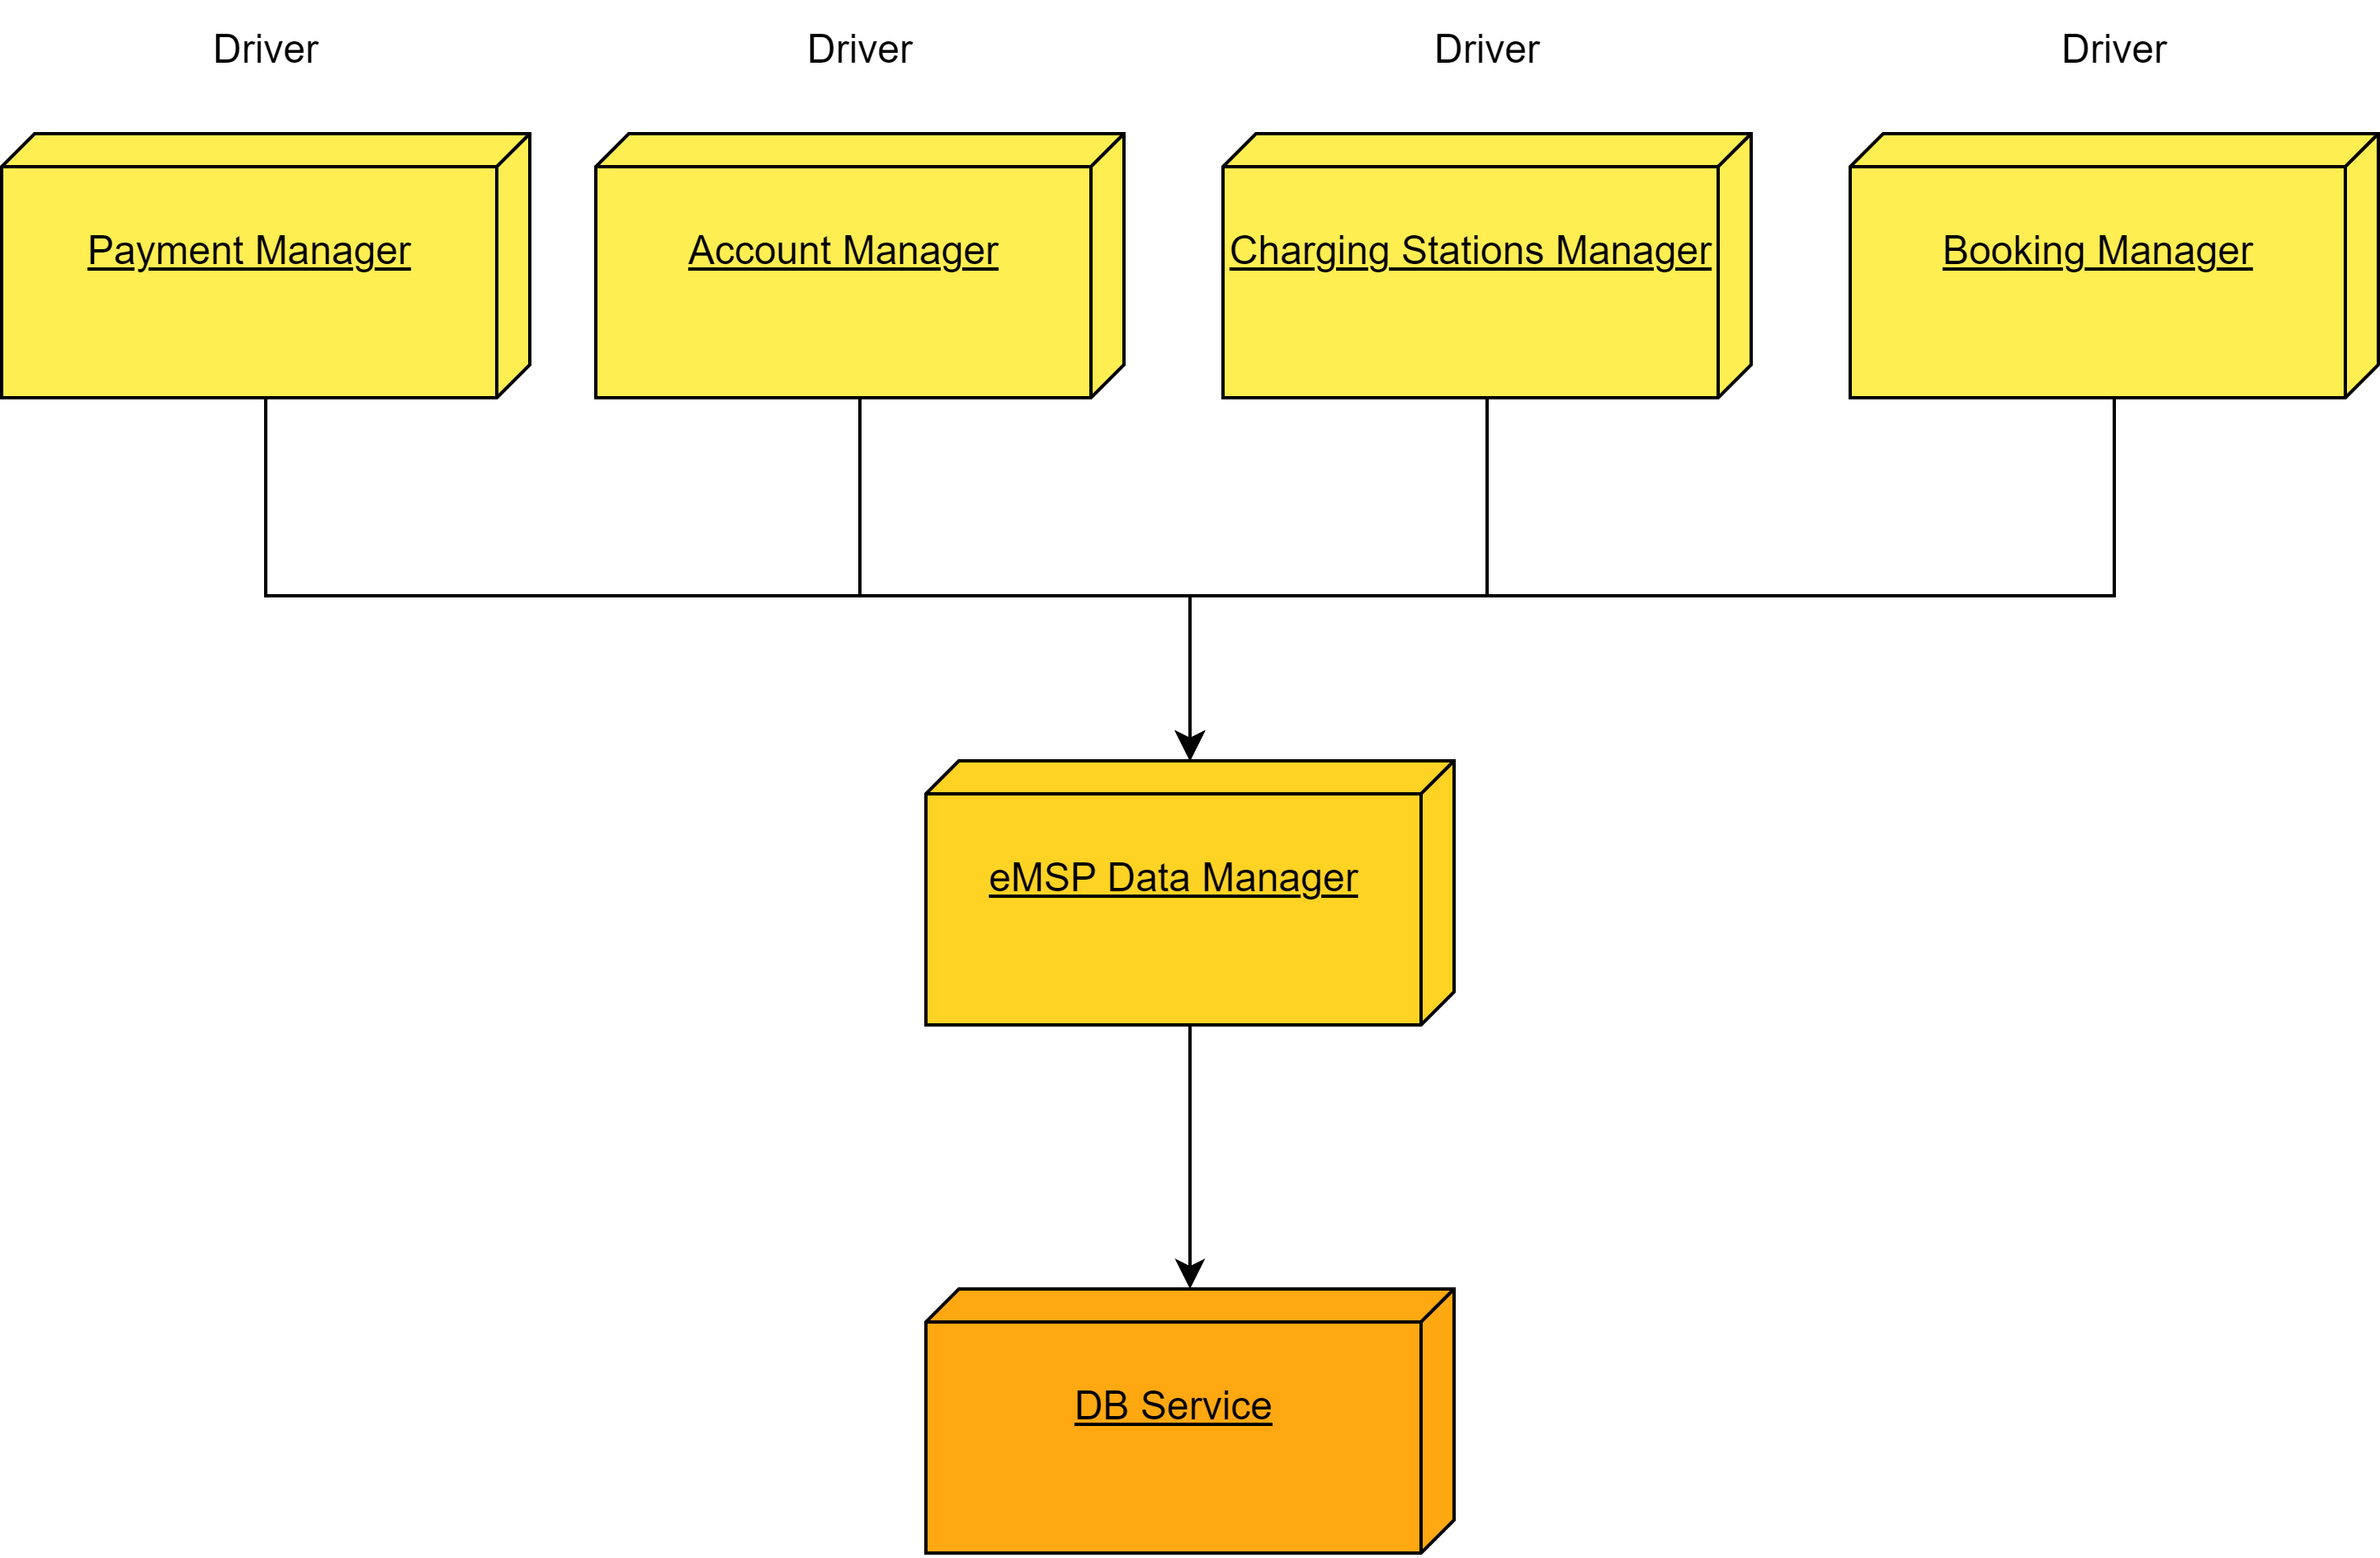
\includegraphics[scale=0.6, center]{assets/Integration Diagrams/eMSP-Data Manager.png}
    \caption{Integration of eMSP-Data Manager}
    \label{fig:eMSP-Data Manager}
\end{figure}
As it was explained before, the Data Manager must be the first one to be implemented as it is the foundation of many other components. For this component, and the following ones of the second and third 
group, drivers emulating components that are not yet implemented are used. The following images represent the implementations of the components of the first group that directly communicate to APIs:
\emph{ Calendar Manager, EV Manager, OCPI, Payment Manager} (Figures 23-26):

\begin{figure}[H]
    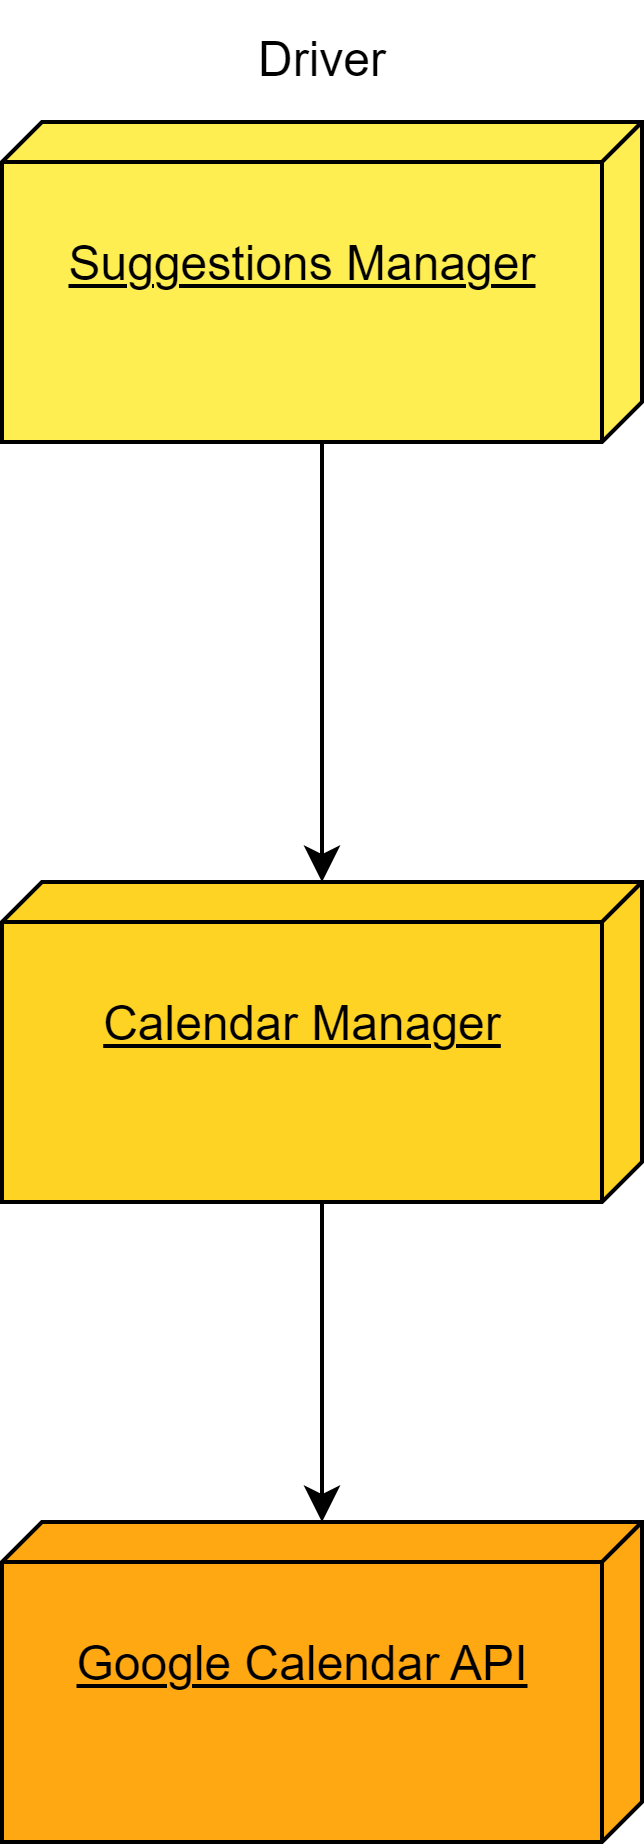
\includegraphics[scale=0.6, center]{assets/Integration Diagrams/eMSP-Calendar Manager.png}
    \caption{Integration of eMSP-Calendar Manager}
    \label{fig:eMSP-Calendar Manager}
\end{figure}

\begin{figure}[H]
    \centering
    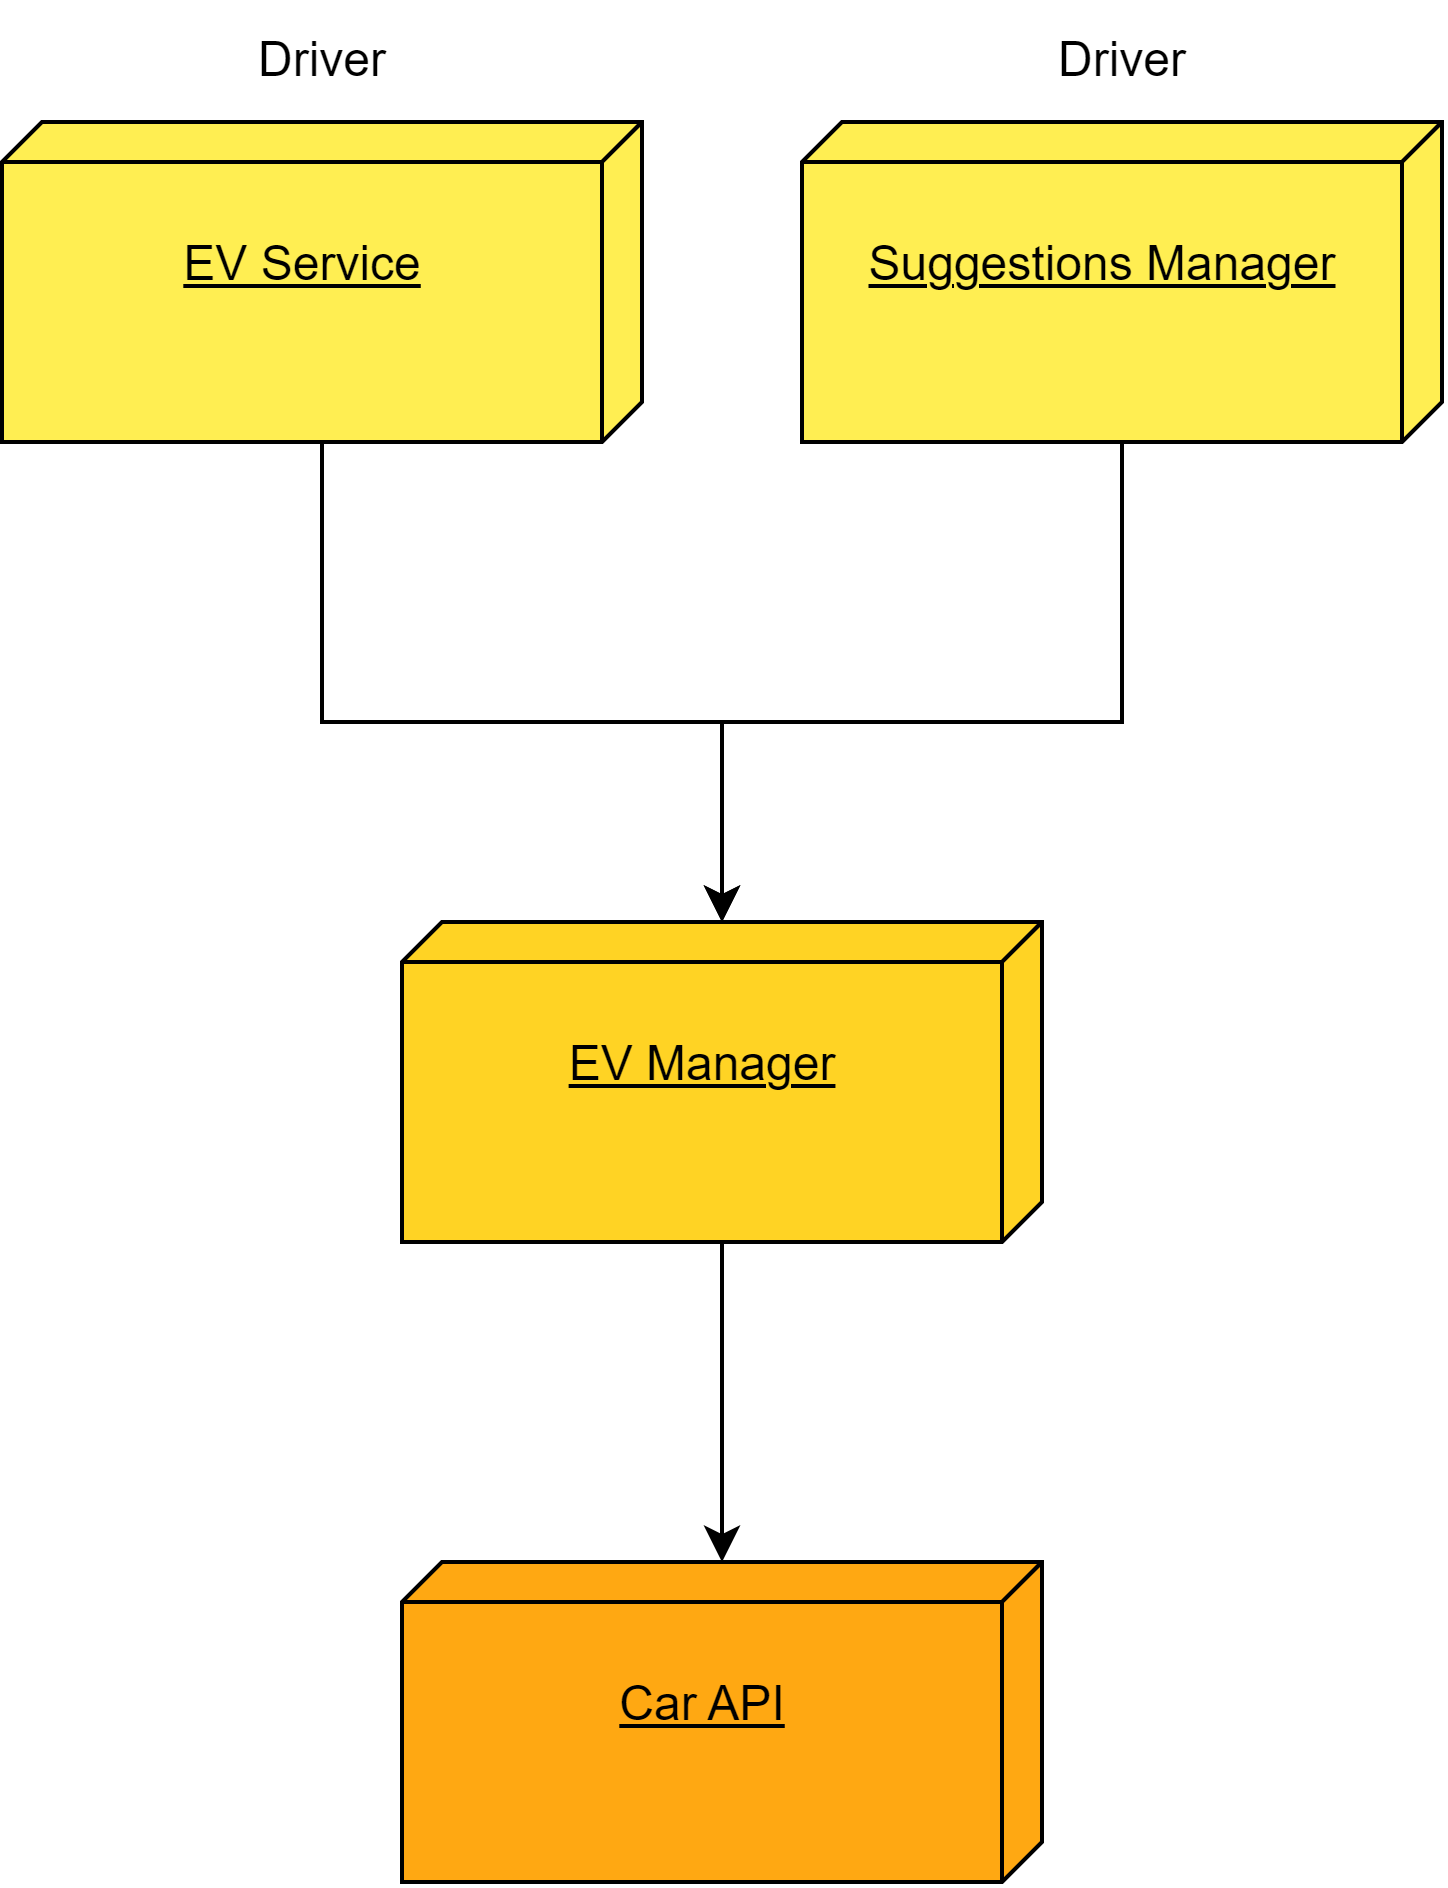
\includegraphics[scale=0.6]{assets/Integration Diagrams/eMSP-EV Manager.png} 
    \caption{Integration of eMSP-EV Manager}%
    \label{fig: eMSP-EV Manager}%
\end{figure}

\begin{figure}[H]
    \centering
    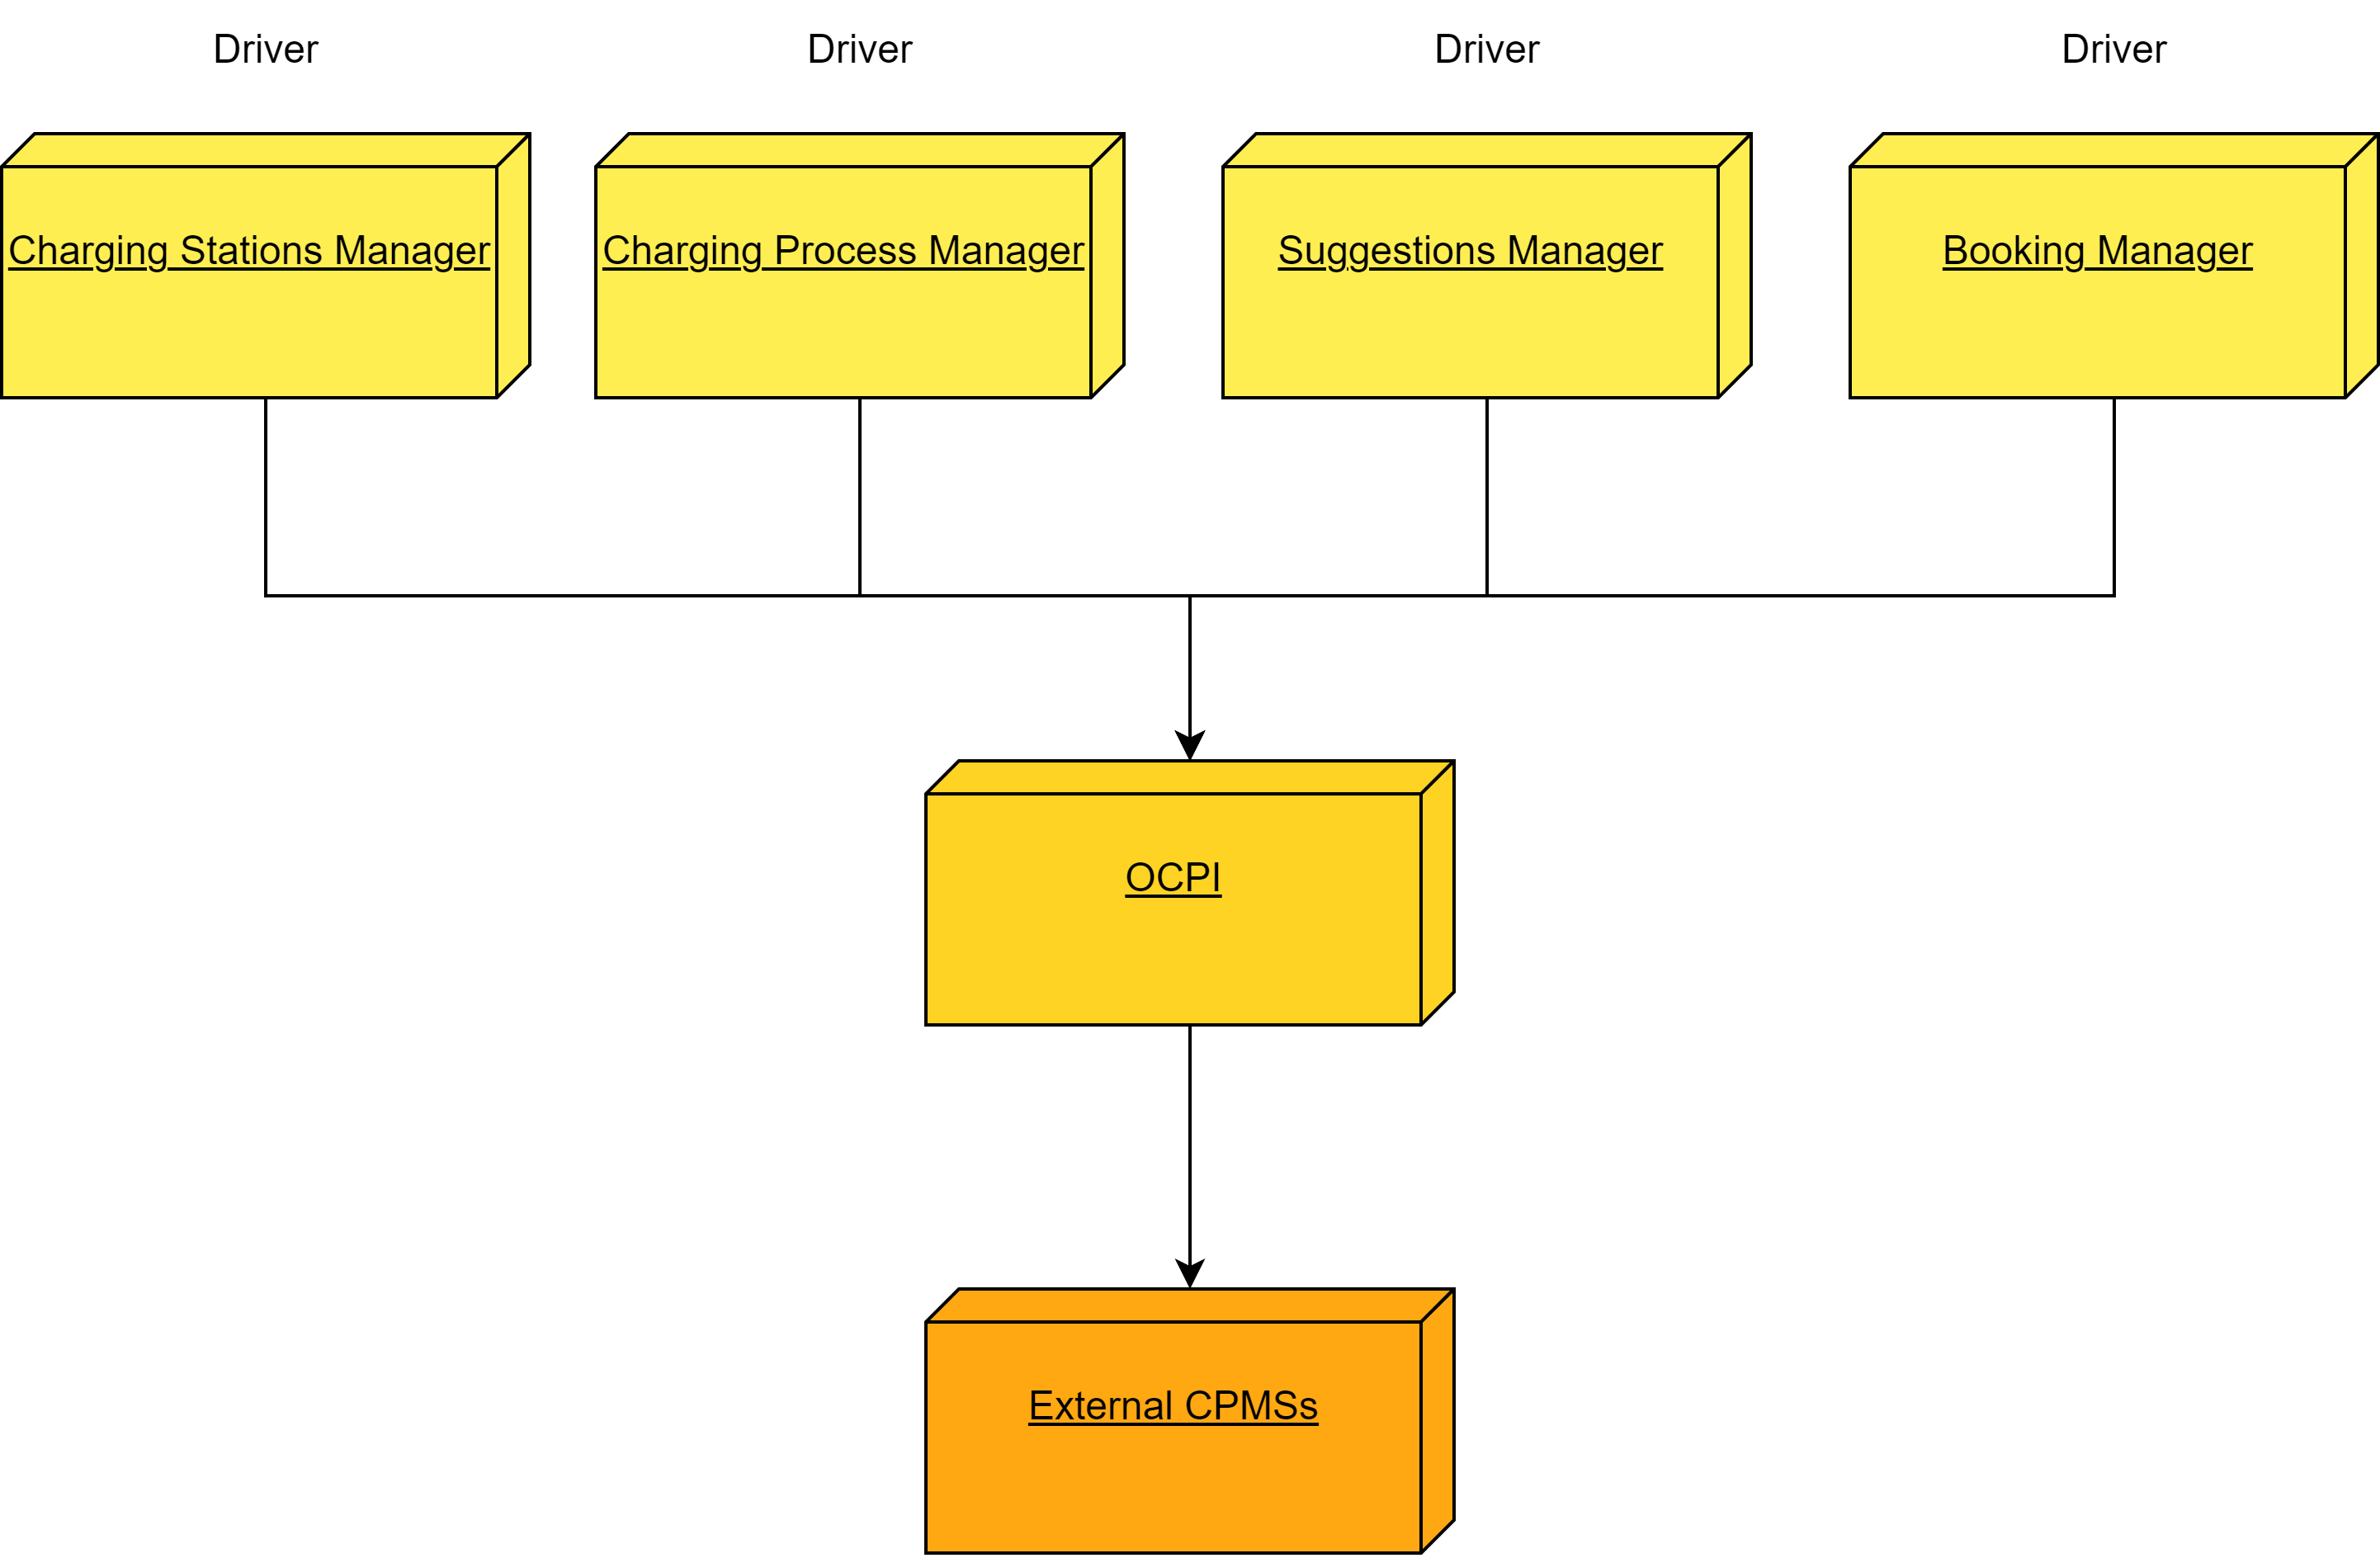
\includegraphics[scale=0.6]{assets/Integration Diagrams/eMSP-OCPI.png} 
    \caption{Integration of eMSP-OCPI}%
    \label{fig: eMSP-OCPI Manager}%
\end{figure}

\begin{figure}[H]
    \centering
    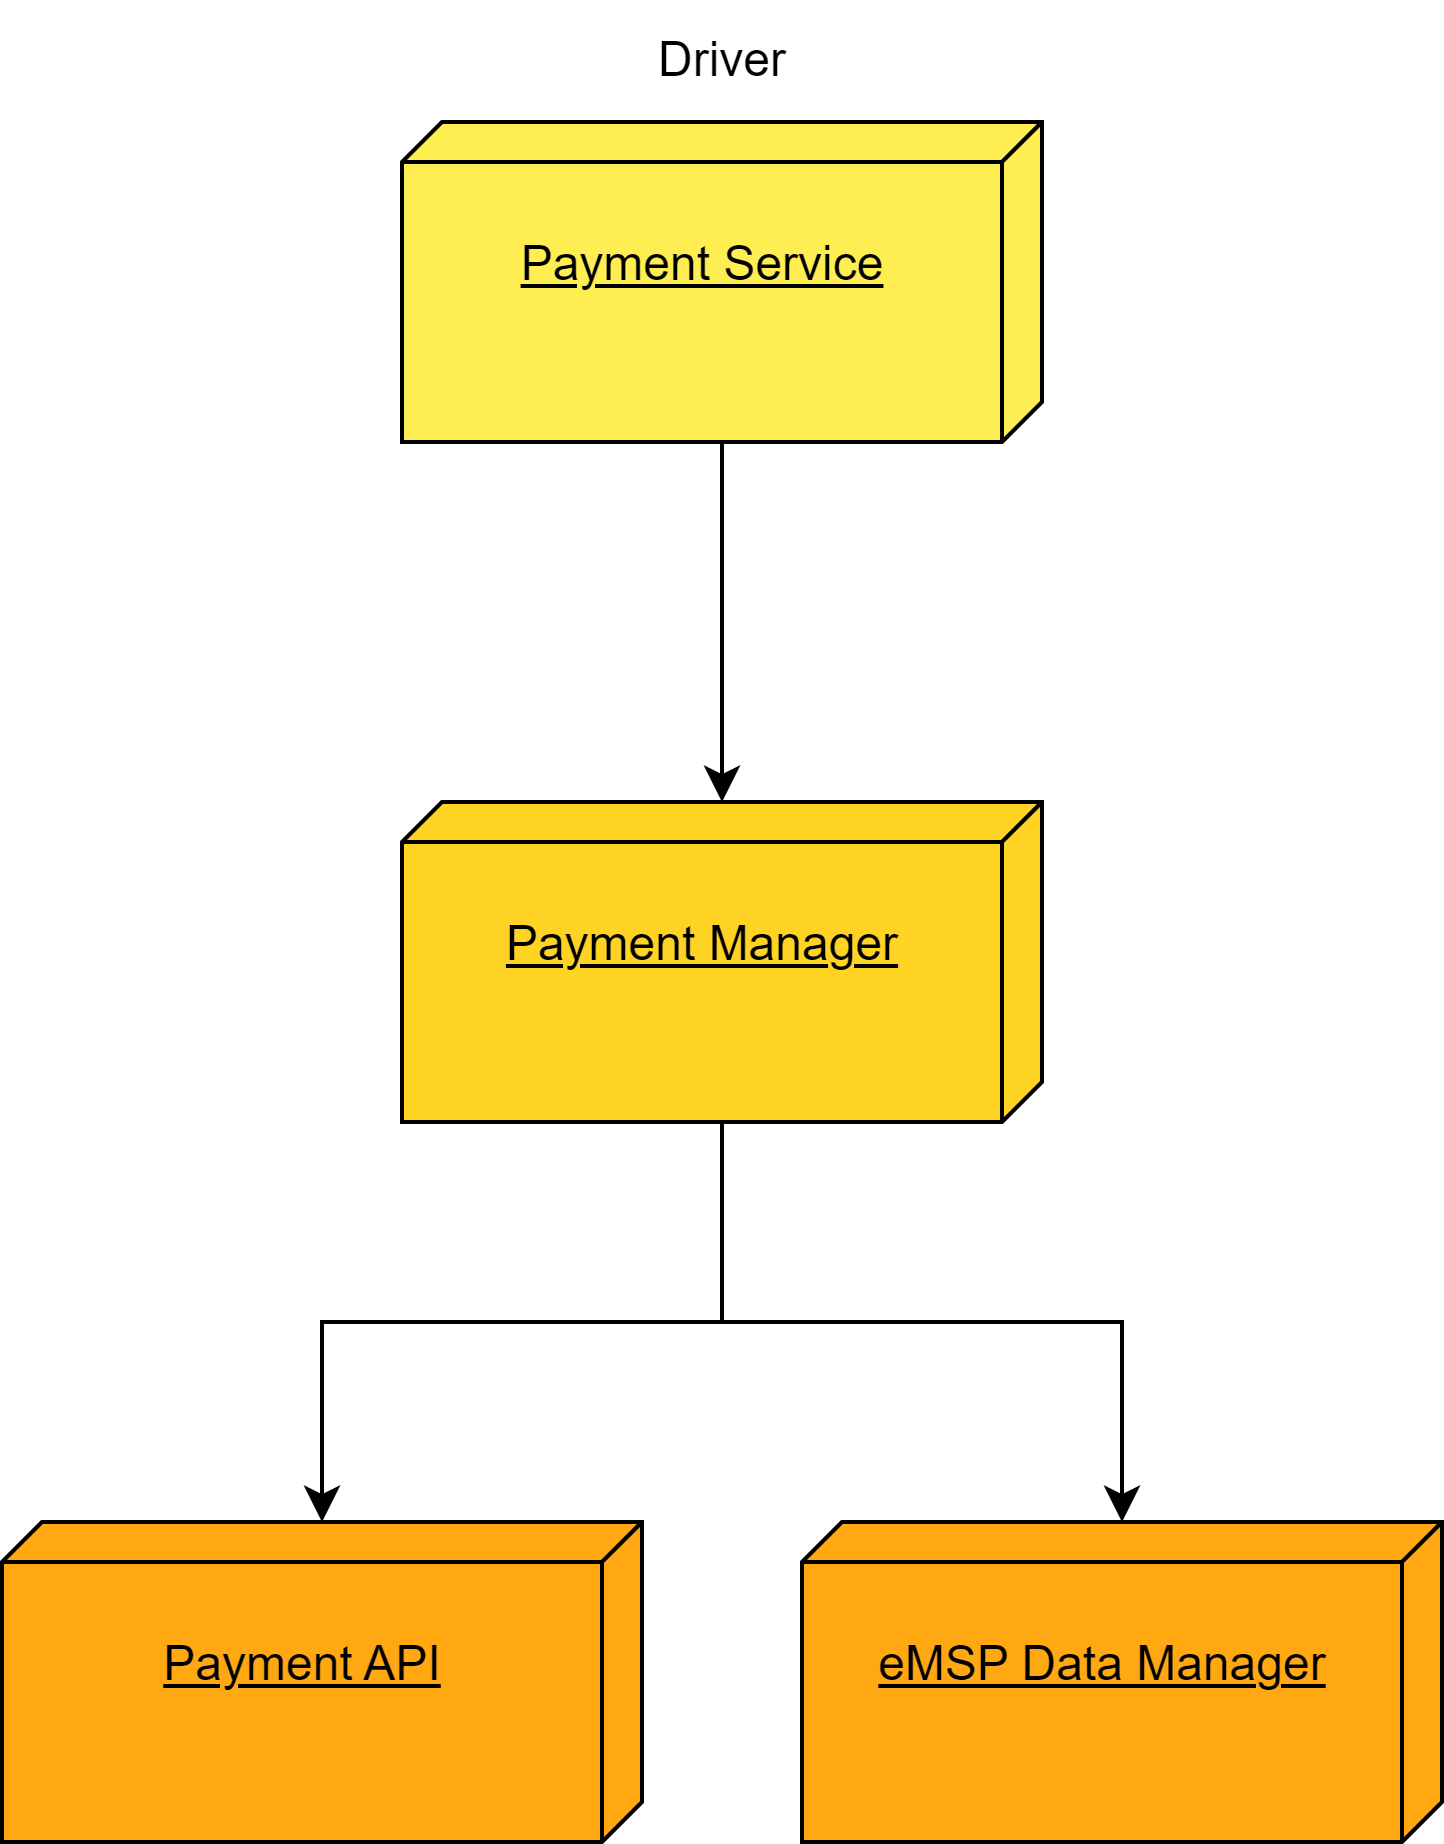
\includegraphics[scale=0.6]{assets/Integration Diagrams/eMSP-Payment Manager.png} 
    \caption{Integration of eMSP-Payment Manager}%
    \label{fig: eMSP-Payment Manager}%
\end{figure}

Following these are the components of the third group, Composed mainly of the Managers that don't interact directly with the APIs but work as a middleman between the service and the data. 
Here are implemented: \emph{ Charging Stations Manager, Charging Process Manager, Booking Manager, Suggestions Manager} (Figures 27-30):

\begin{figure}[H]
    \centering
    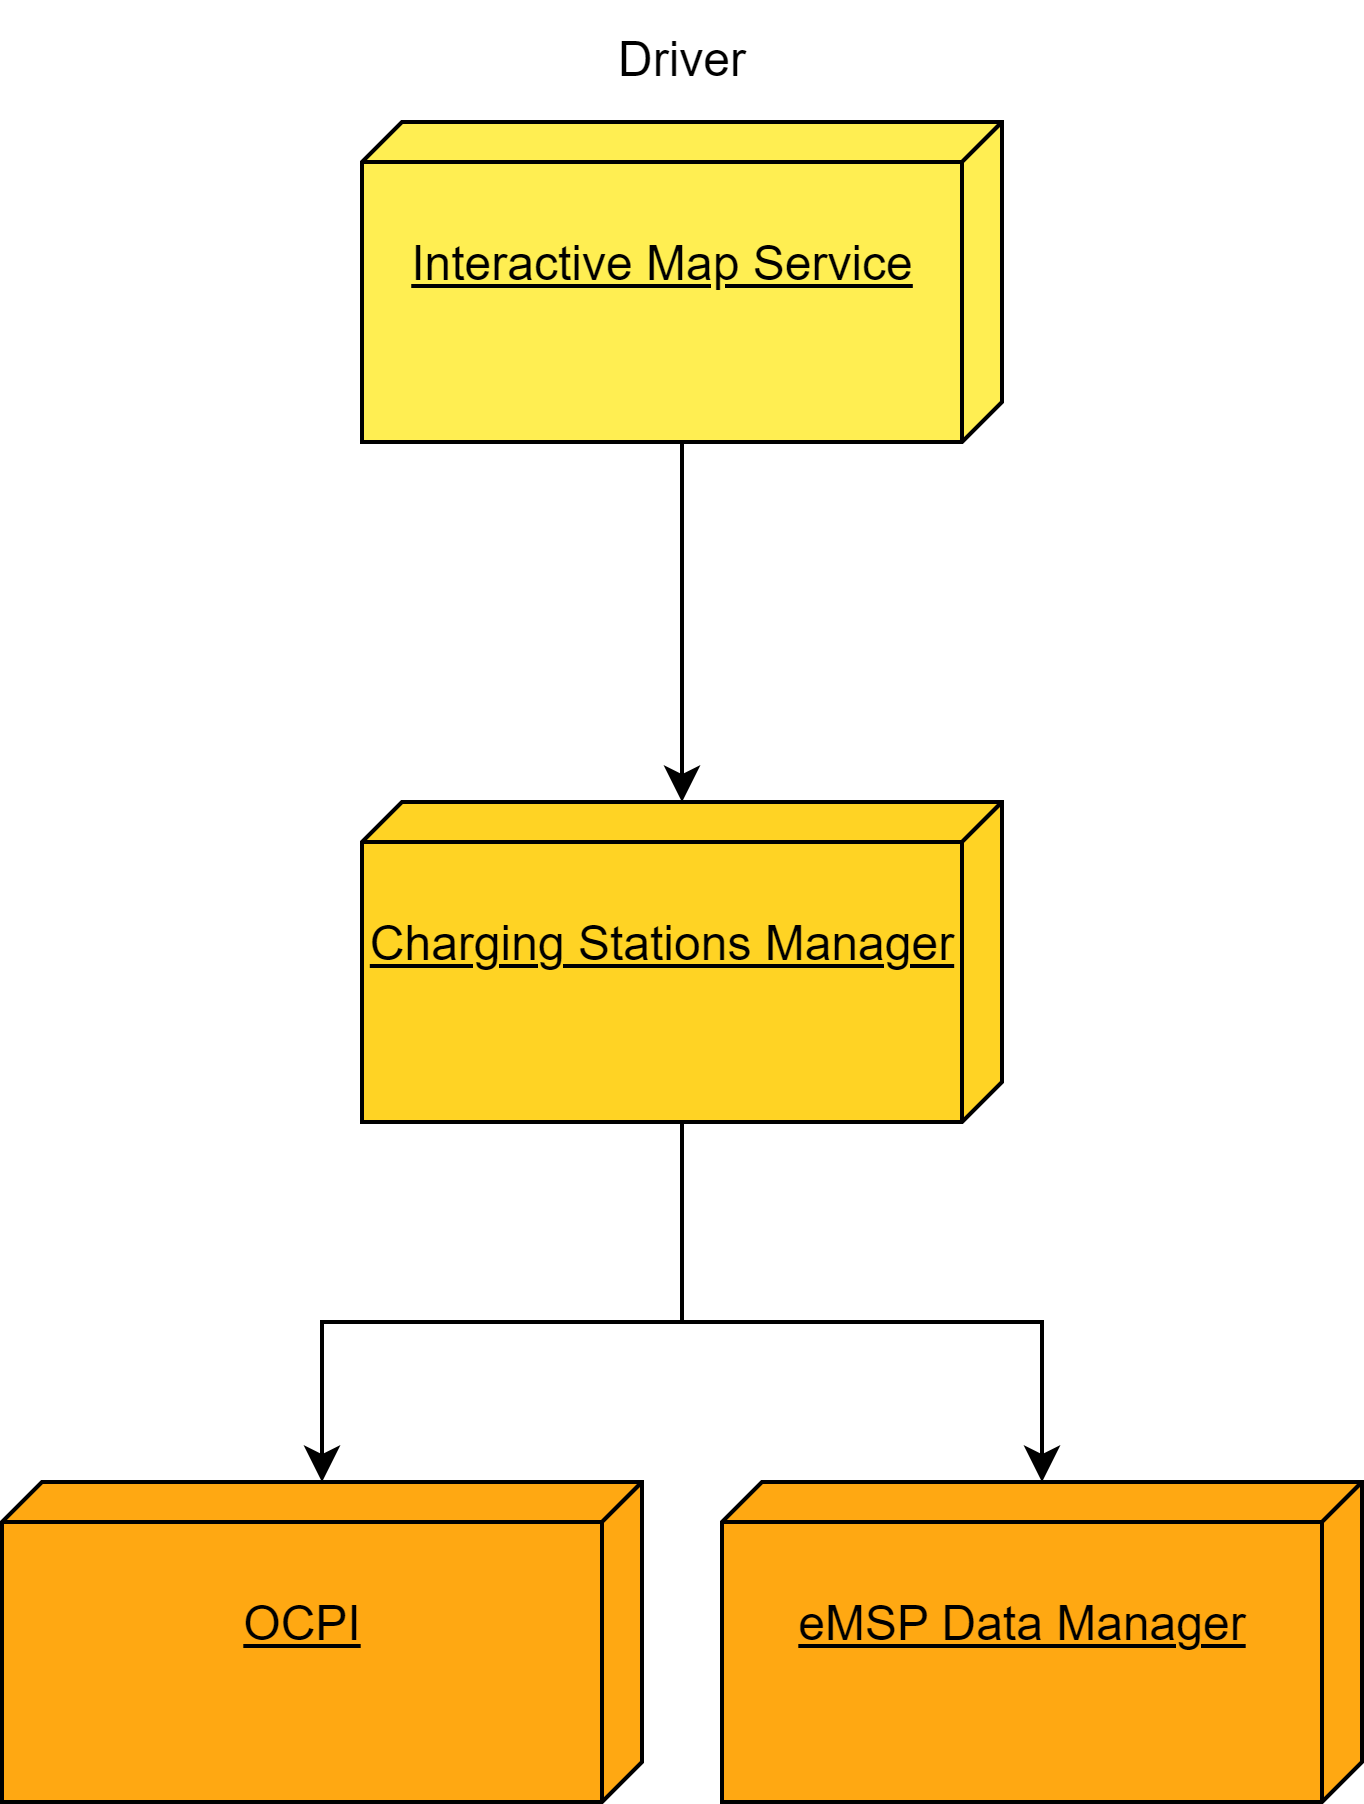
\includegraphics[scale=0.6]{assets/Integration Diagrams/eMSP-Charging stations manager.png} 
    \caption{Integration of eMSP-Charging Stations manager}%
    \label{fig: eMSP-Charging Stations manager}%
\end{figure}

\begin{figure}[H]
    \centering
    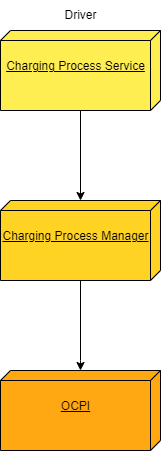
\includegraphics[scale=0.6]{assets/Integration Diagrams/eMSP-Charging Process Manager.png} 
    \caption{Integration of eMSP-Charging Process Manager}%
    \label{fig: eMSP-Charging Process Manager}%
\end{figure}

\begin{figure}[H]
    \centering
    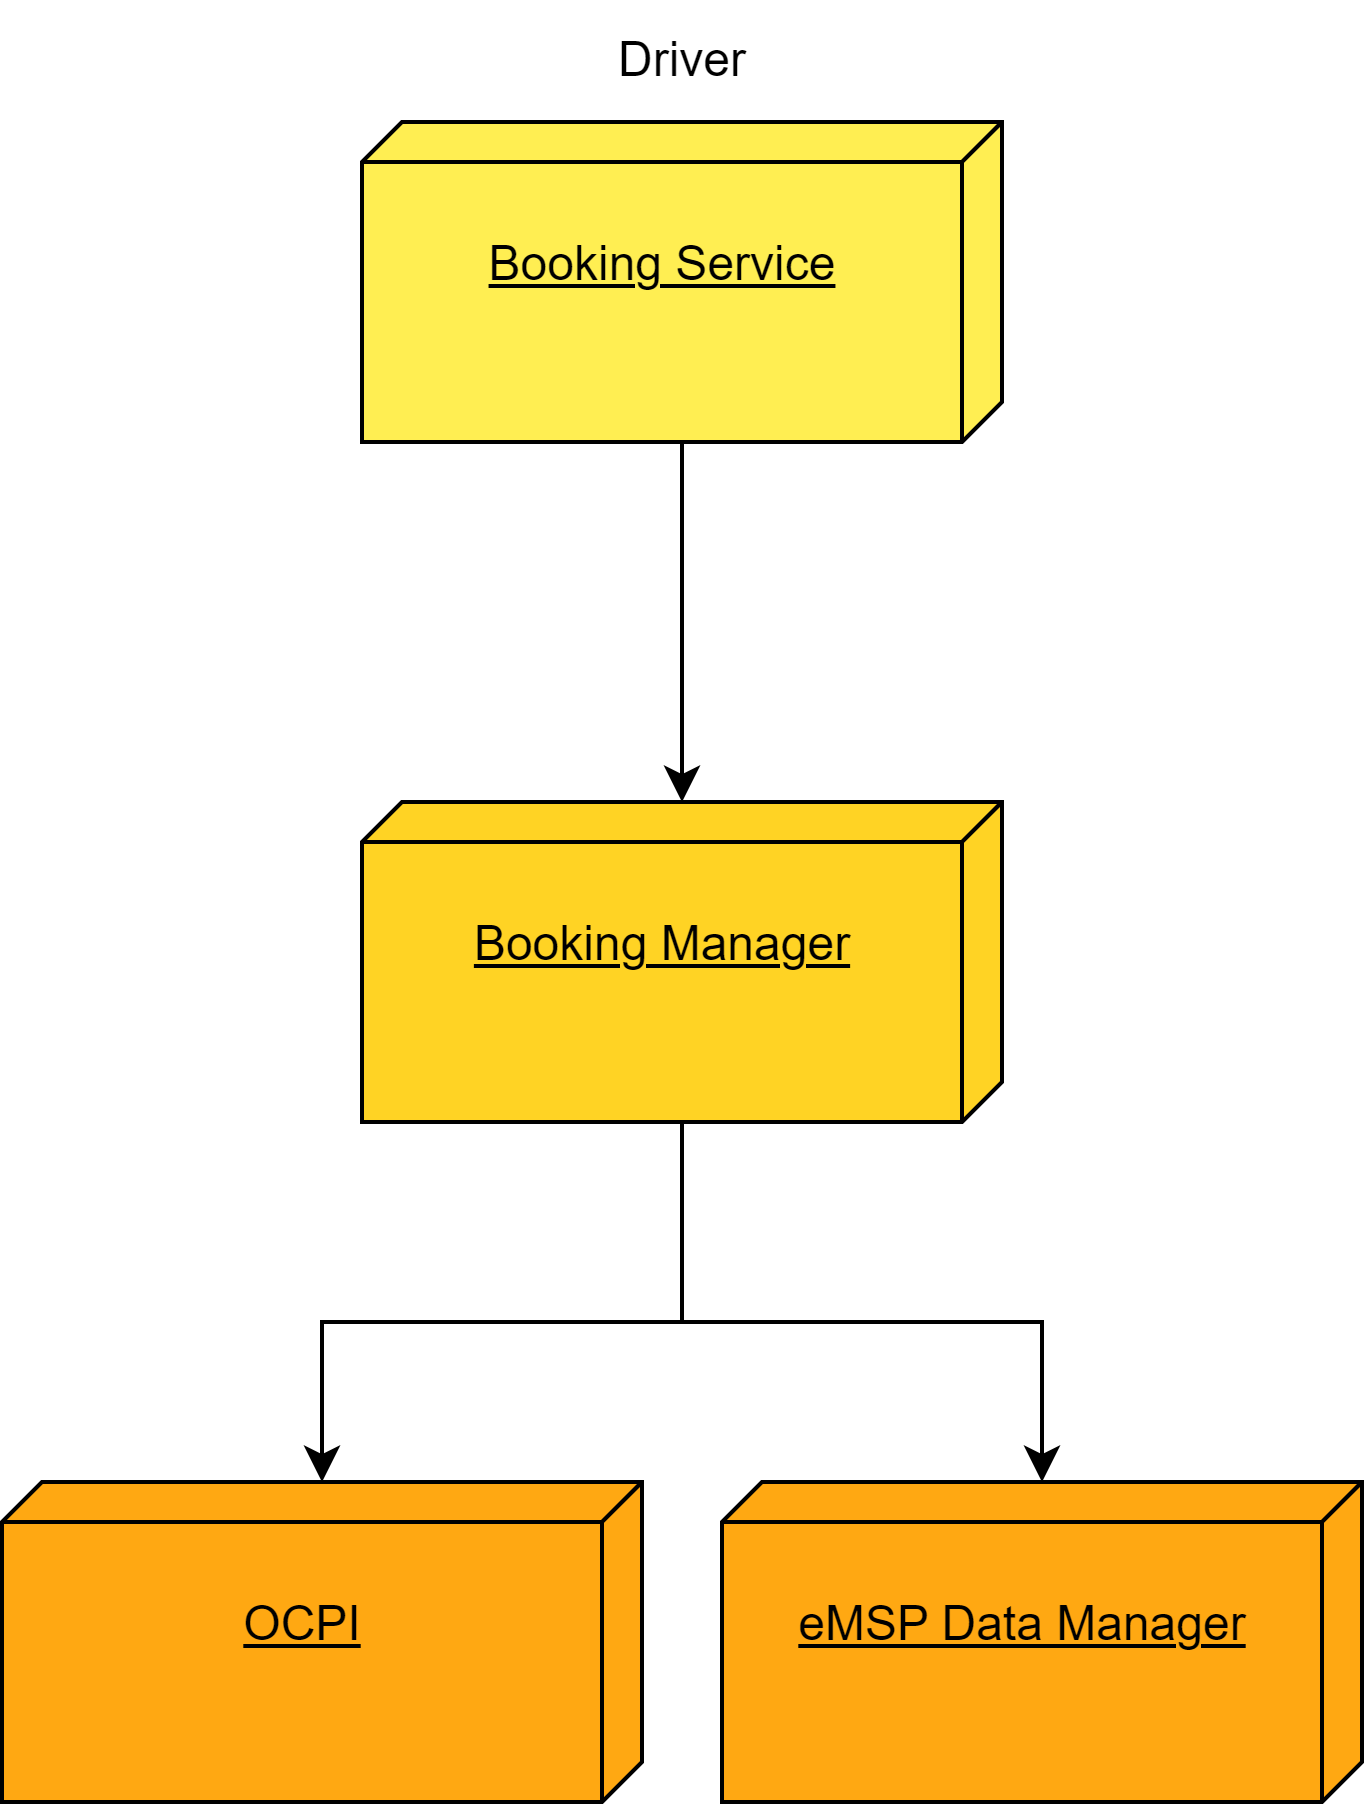
\includegraphics[scale=0.6]{assets/Integration Diagrams/eMSP-Booking Manager.png} 
    \caption{Integration of eMSP-Booking manager}%
    \label{fig: eMSP-Booking manager}%
\end{figure}

\begin{figure}[H]
    \centering
    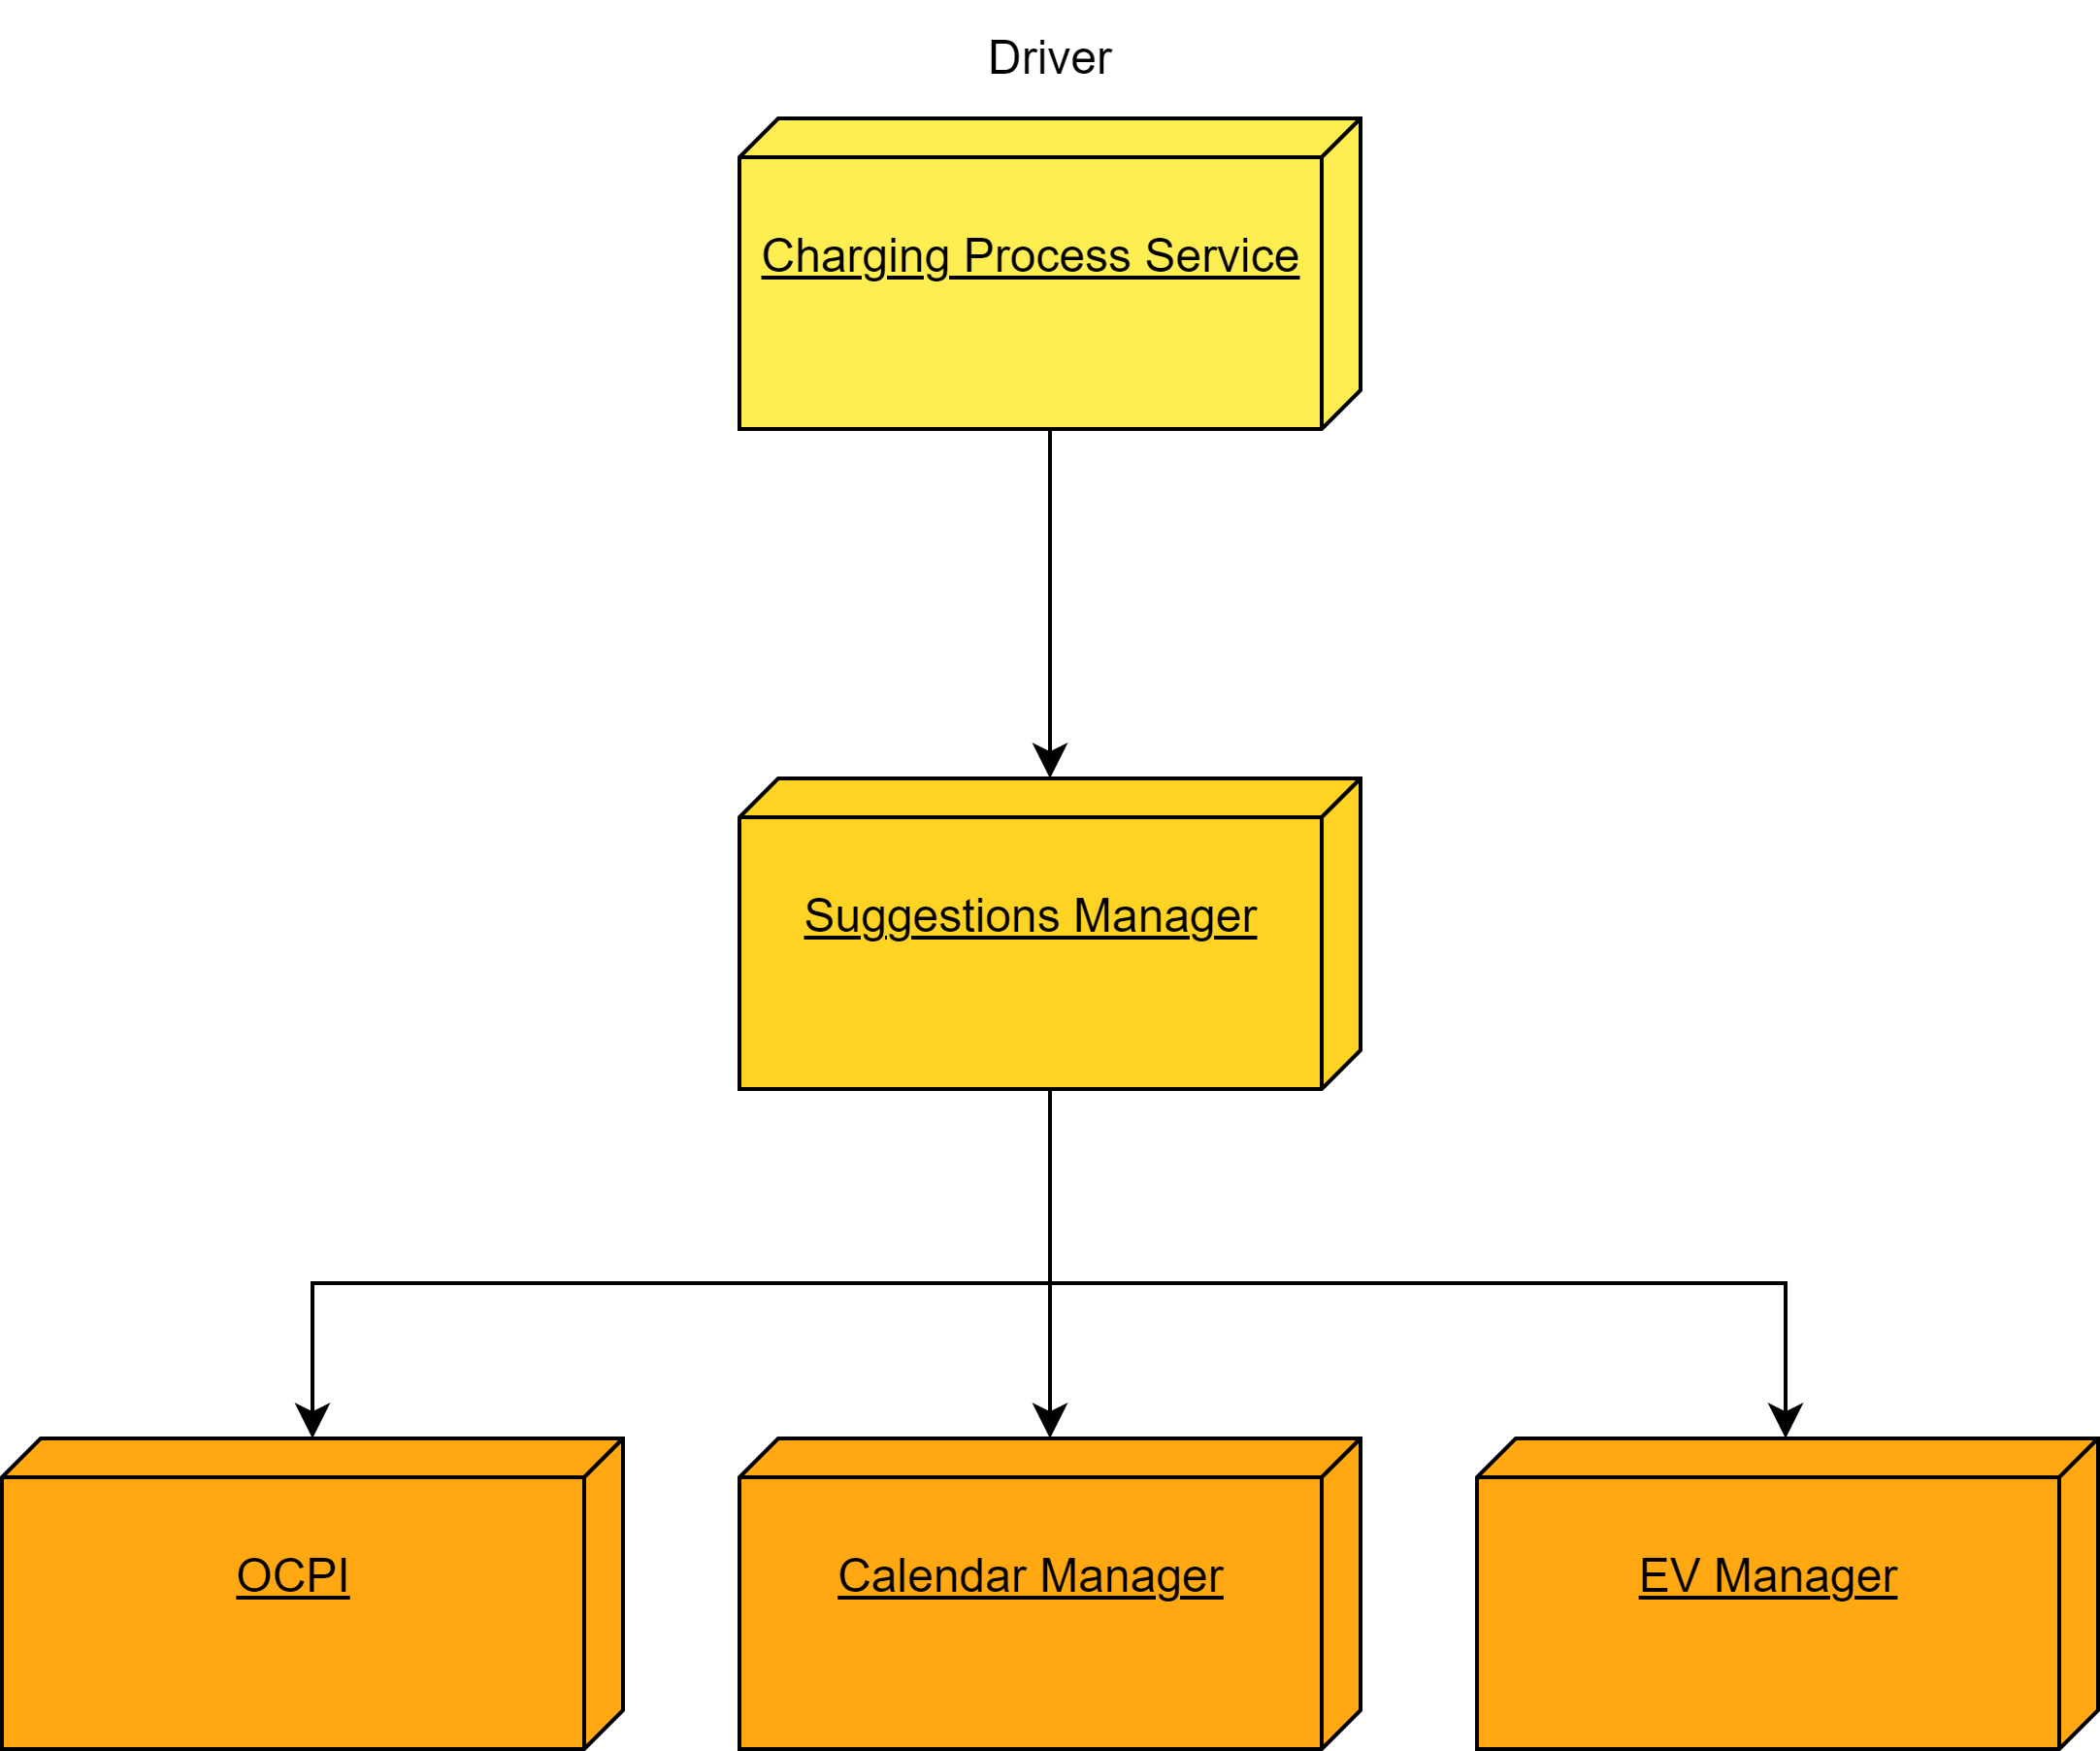
\includegraphics[scale=0.6]{assets/Integration Diagrams/eMSP-Suggestions Manager.png} 
    \caption{Integration of eMSP-Suggestion manager}%
    \label{fig: eMSP-Suggestion manager}%
\end{figure}

Lastly are the Integrations of the most external devices, the services. At this point of the integration no drivers are needed anymore.
Here are represented \emph{Account Manager} and \emph{User Manager}, considering that they both encapsulate services.

\begin{figure}[H]
    \centering
    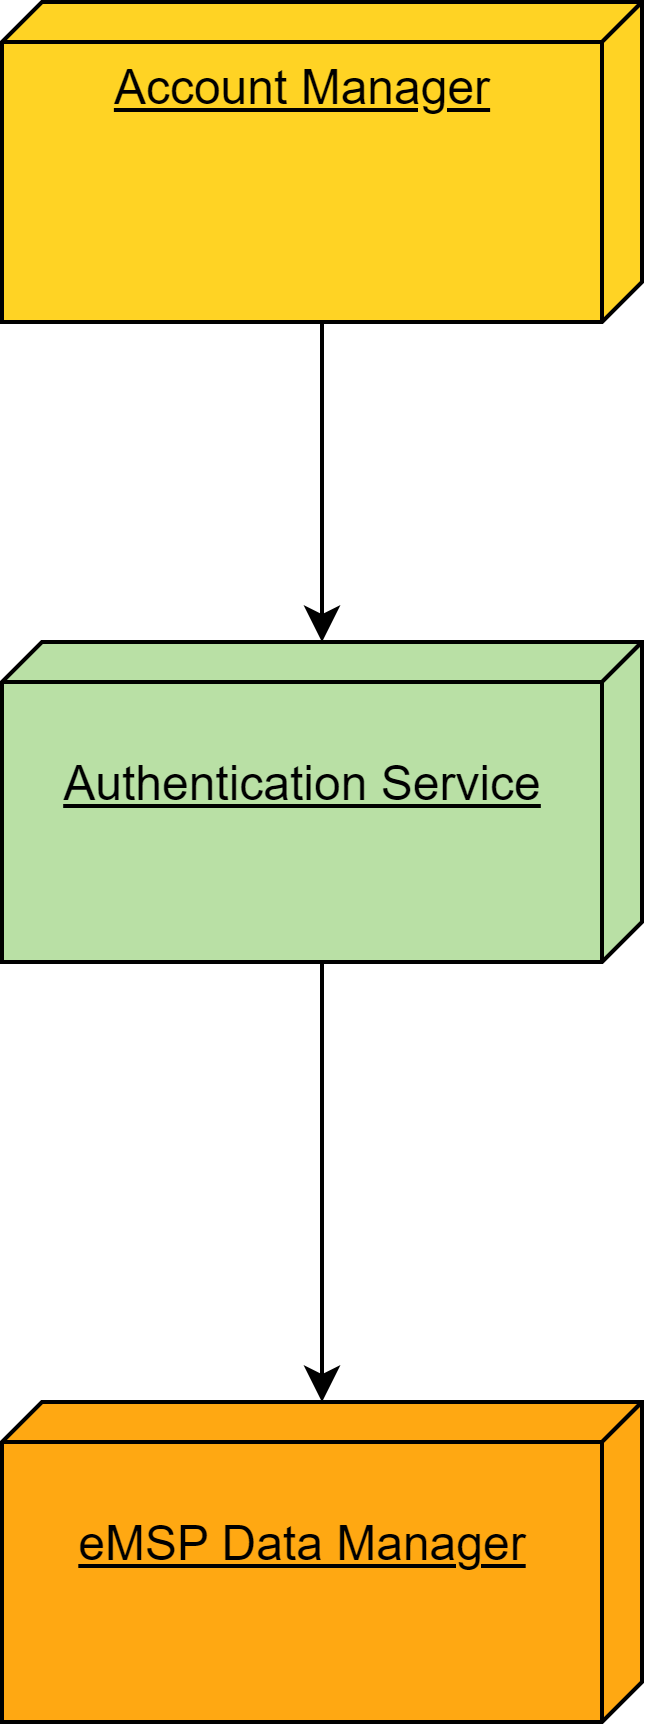
\includegraphics[scale=0.6]{assets/Integration Diagrams/eMSP-Account Manager.png} 
    \caption{Integration of eMSP-Account Manager}%
    \label{fig: eMSP-Account Manager}%
\end{figure}

\begin{figure}[H]
    \centering
    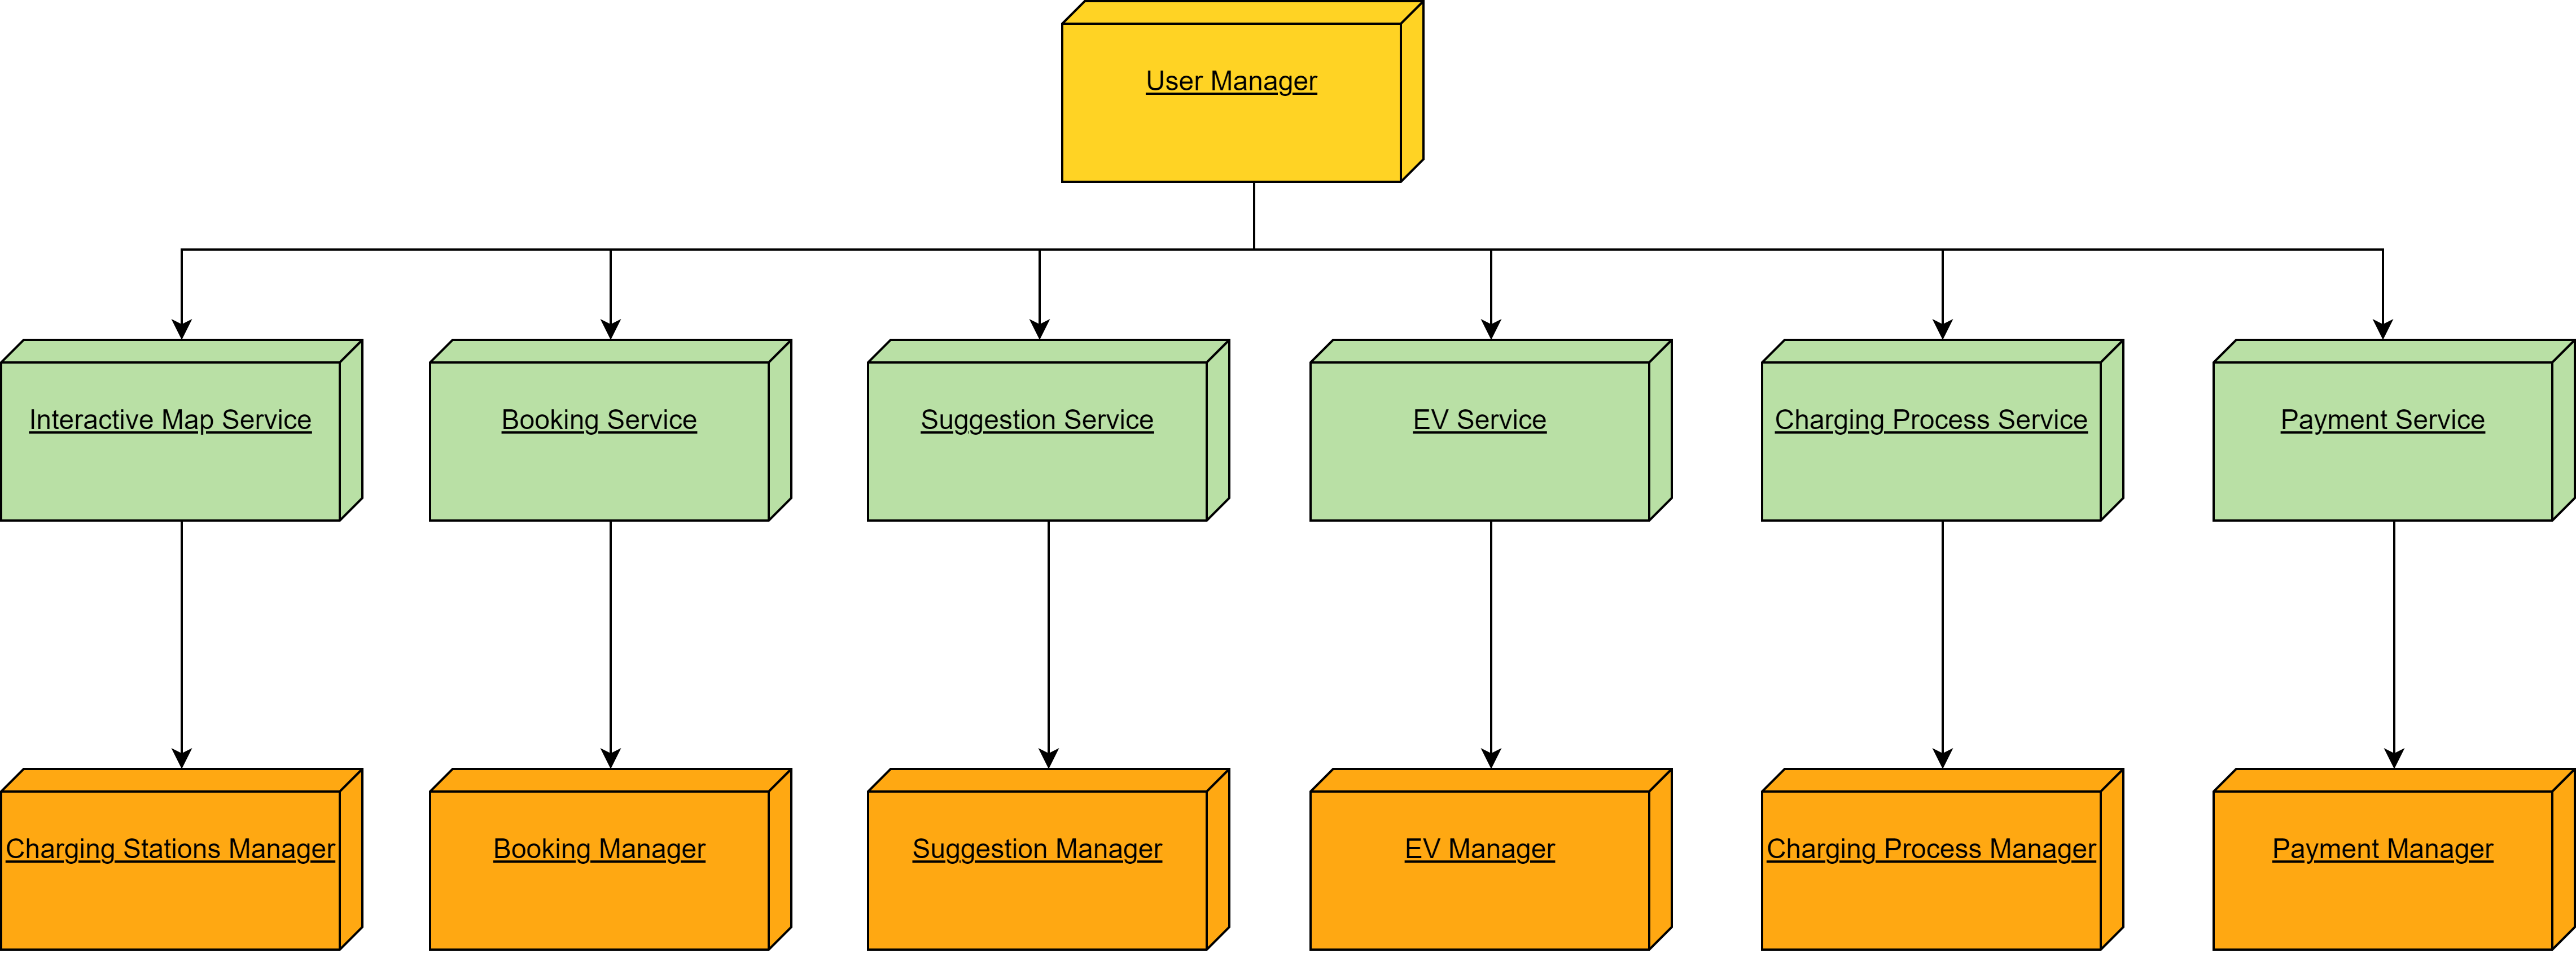
\includegraphics[scale=0.6]{assets/Integration Diagrams/eMSP-User Manager.png} 
    \caption{Integration of eMSP-User manager}%
    \label{fig: eMSP-User manager}%
\end{figure}

\newpage
\textbf{CPMS Subsystem} \newline
In the same way we dealt with the eMSP, we will now present the various integration of the components. As already stated, the order in which the whole subsystems are implemented is 
completely up to preference, as they are independent. \newline
In the case of the CPMS we have a further independence between the \emph{Data Manager} and the other API managers, so they all could parallelize, hence why they are all within that first group.
Here they are all represented:

\begin{figure}[H]
    \centering
    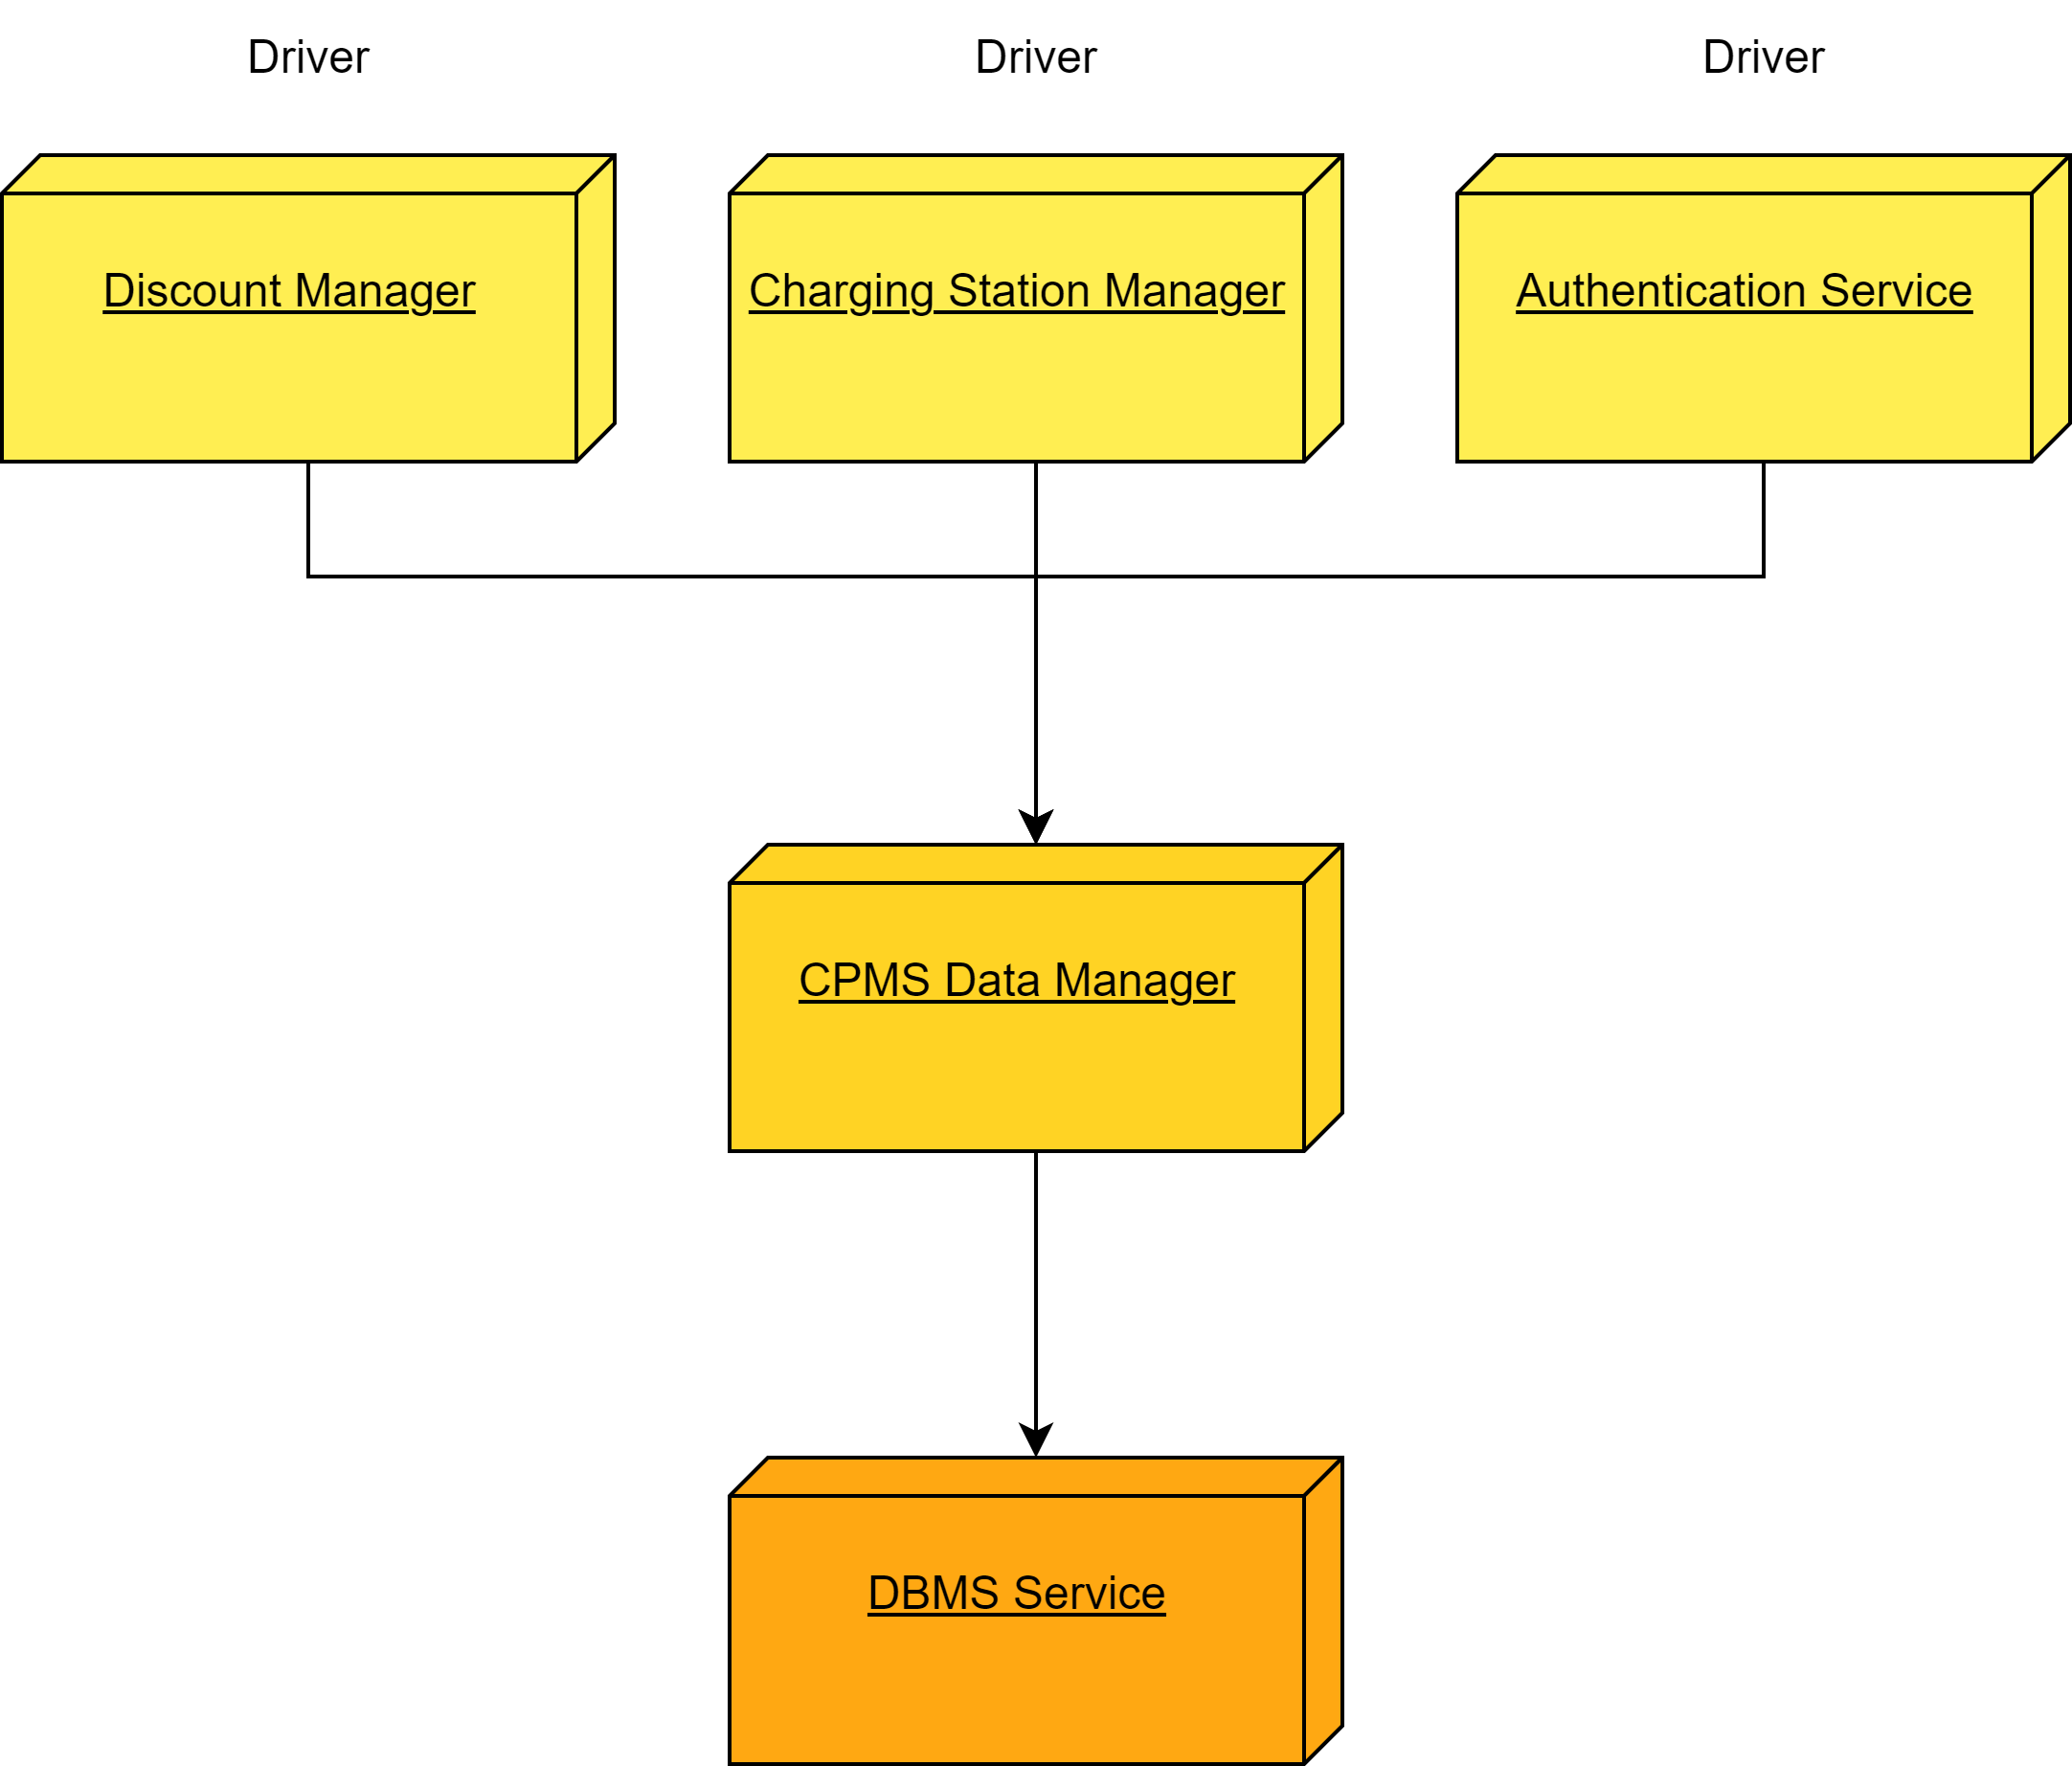
\includegraphics[scale=0.6]{assets/Integration Diagrams/CPMS-Data Manager.png} 
    \caption{Integration of CPMS-Data Manager}%
    \label{fig: CPMS-Data manager}%
\end{figure}

\begin{figure}[H]
    \centering
    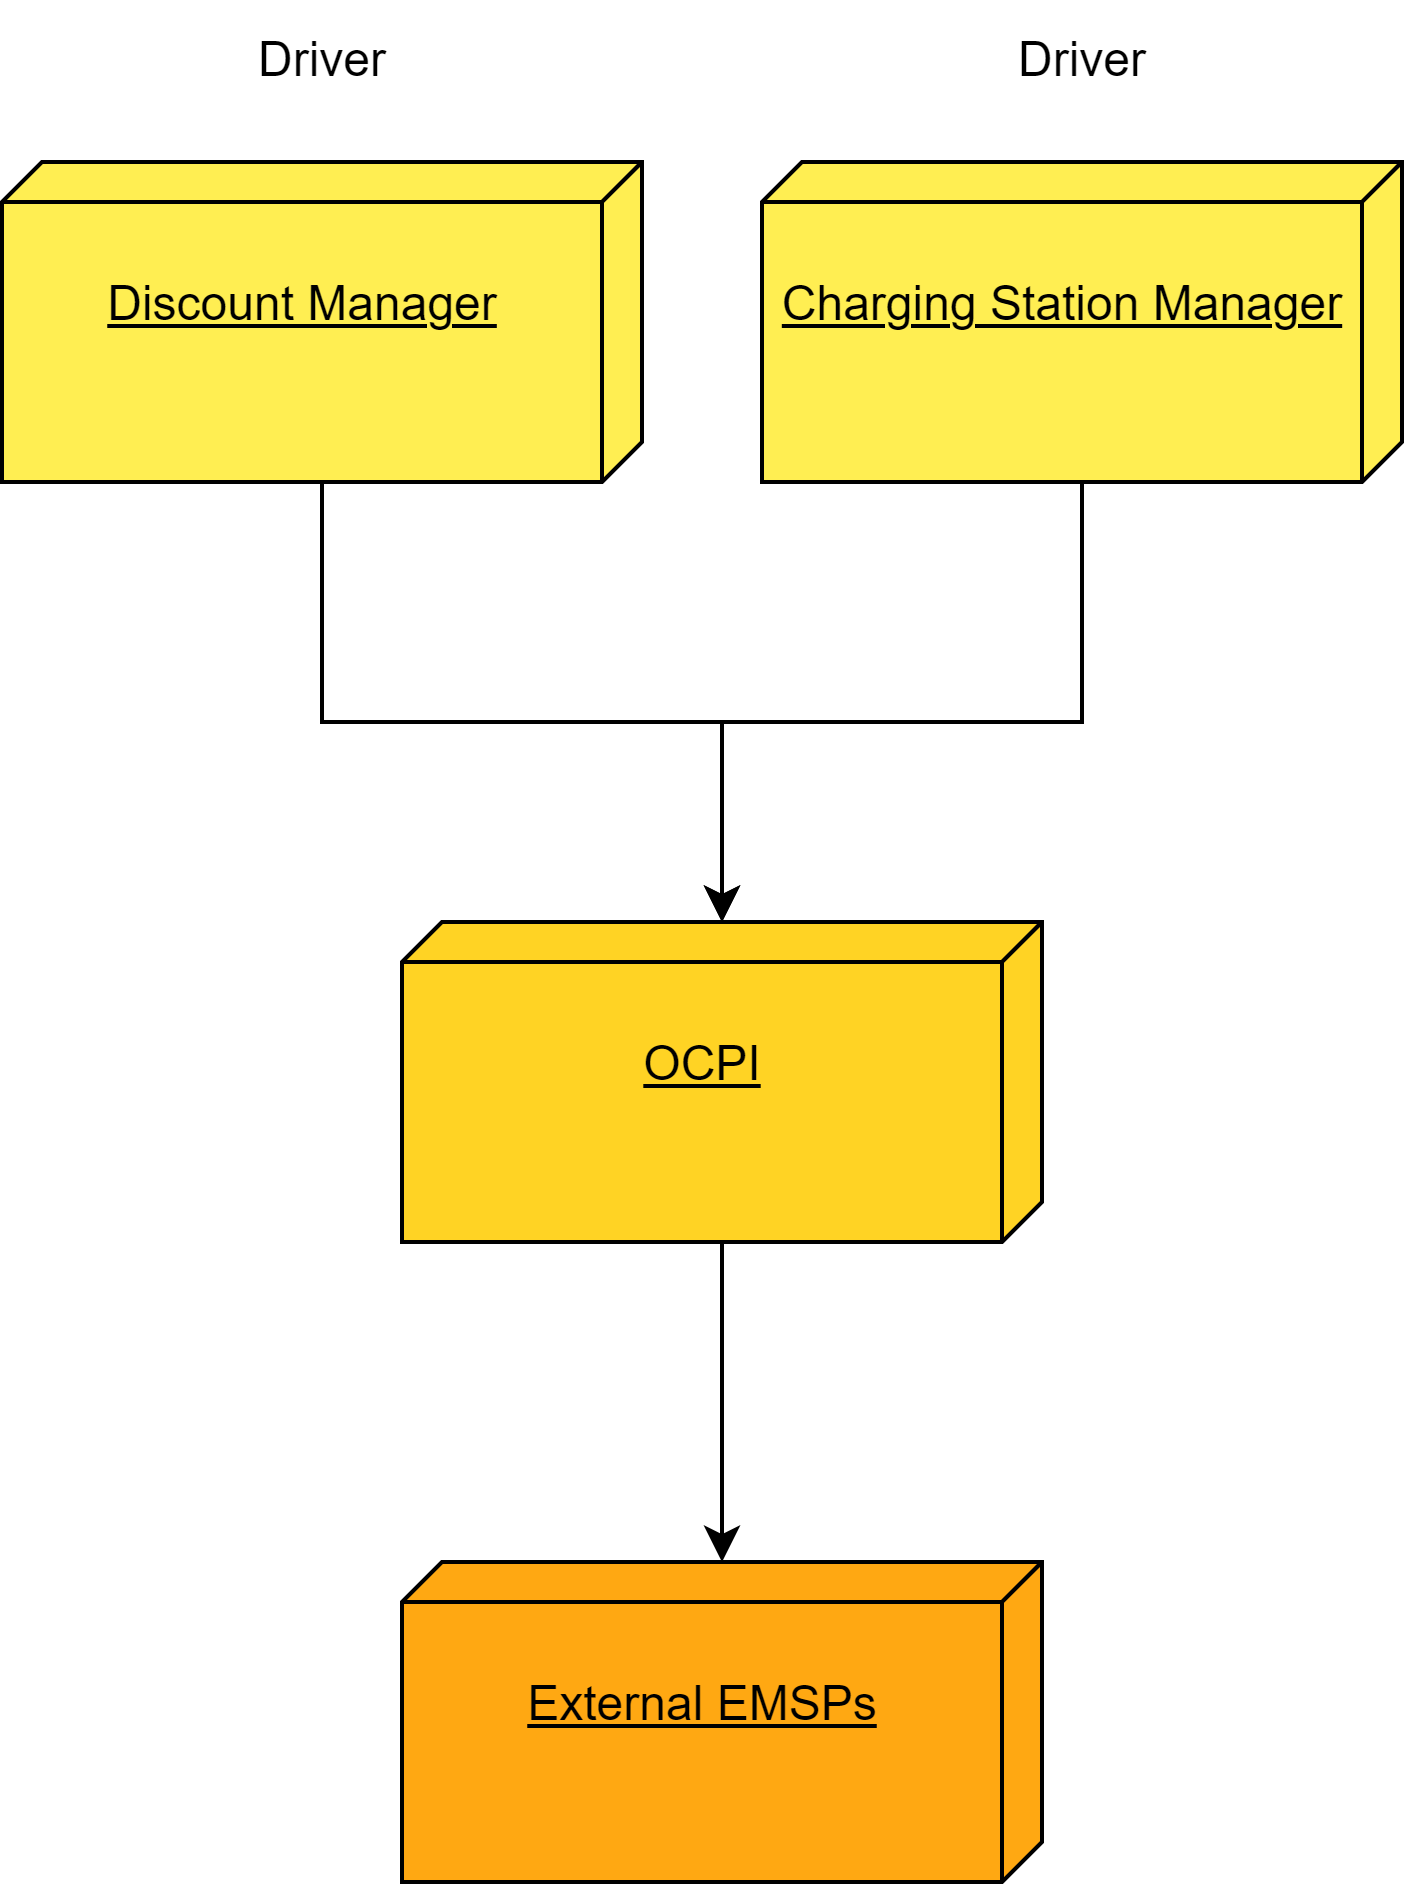
\includegraphics[scale=0.6]{assets/Integration Diagrams/CPMS-OCPI.png} 
    \caption{Integration of CPMS-OCPI}%
    \label{fig: CPMS-OCPI}%
\end{figure}

\begin{figure}[H]
    \centering
    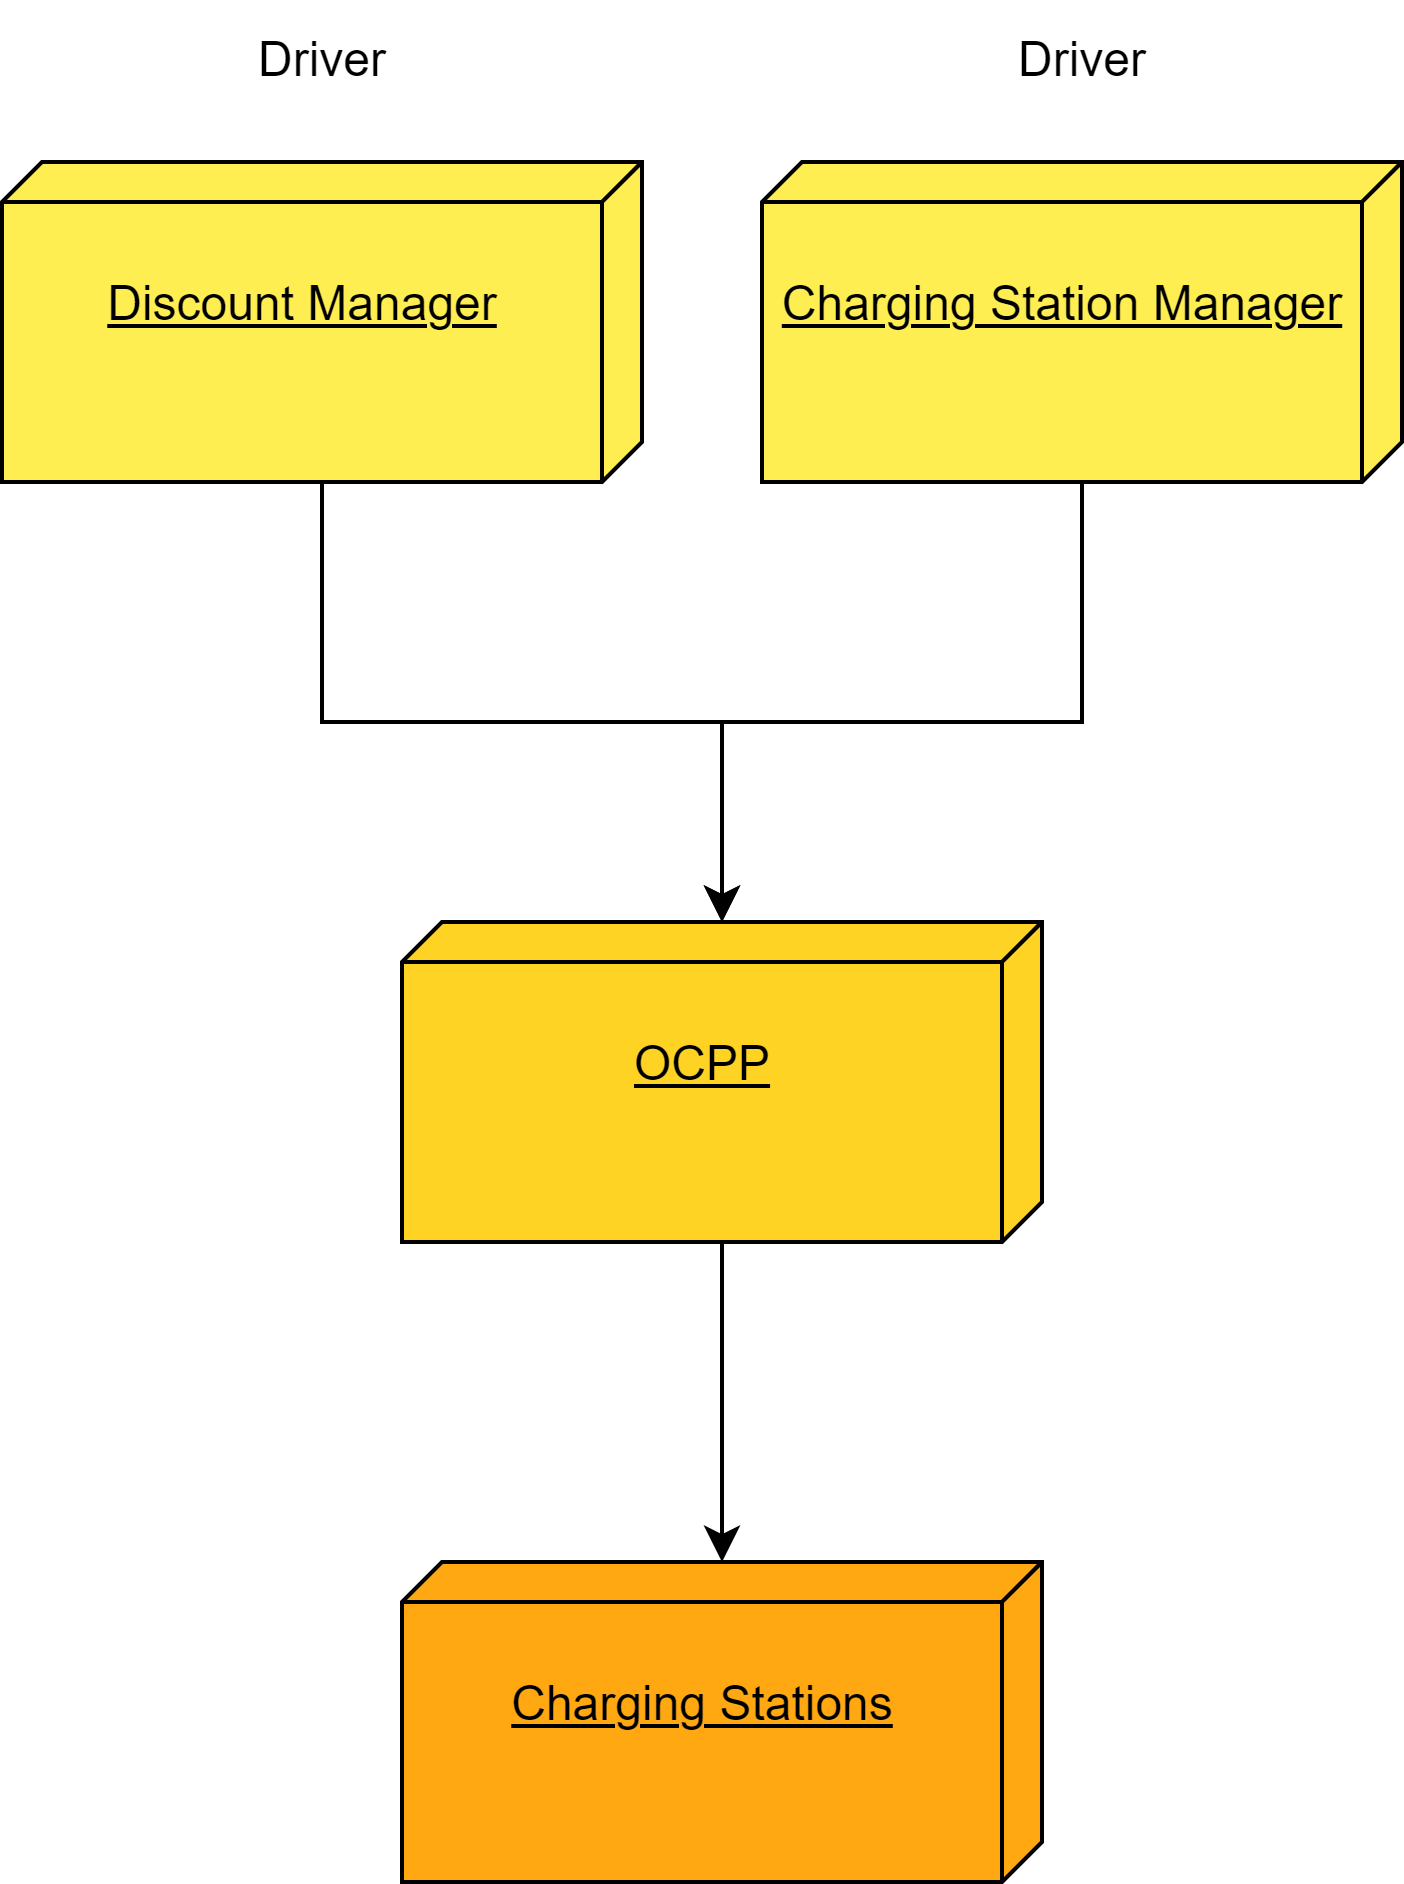
\includegraphics[scale=0.6]{assets/Integration Diagrams/CPMS-OCPP.png} 
    \caption{Integration of CPMS-OCPP}%
    \label{fig: CPMS-OCPP}%
\end{figure}

\begin{figure}[H]
    \centering
    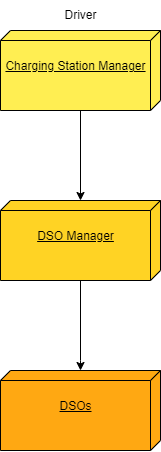
\includegraphics[scale=0.6]{assets/Integration Diagrams/CPMS-DSO Manager.png} 
    \caption{Integration of CPMS-DSO Manager}%
    \label{fig: CPMS-DSO Manager}%
\end{figure}

In the second group, we have \emph{Discount Manager} and \emph{Charging Station Manager}, the components that act as a middlemen between the services and the APIs.
Here they are represented:

\begin{figure}[H]
    \centering
    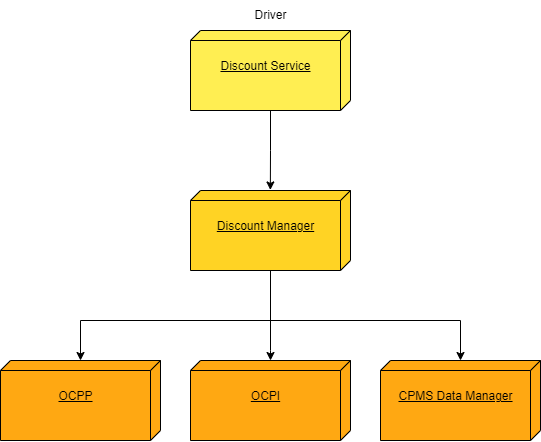
\includegraphics[scale=0.6]{assets/Integration Diagrams/CPMS-Discount Manager.png} 
    \caption{Integration of CPMS-Discount Manager}%
    \label{fig: CPMS-Discount Manager}%
\end{figure}

\begin{figure}[H]
    \centering
    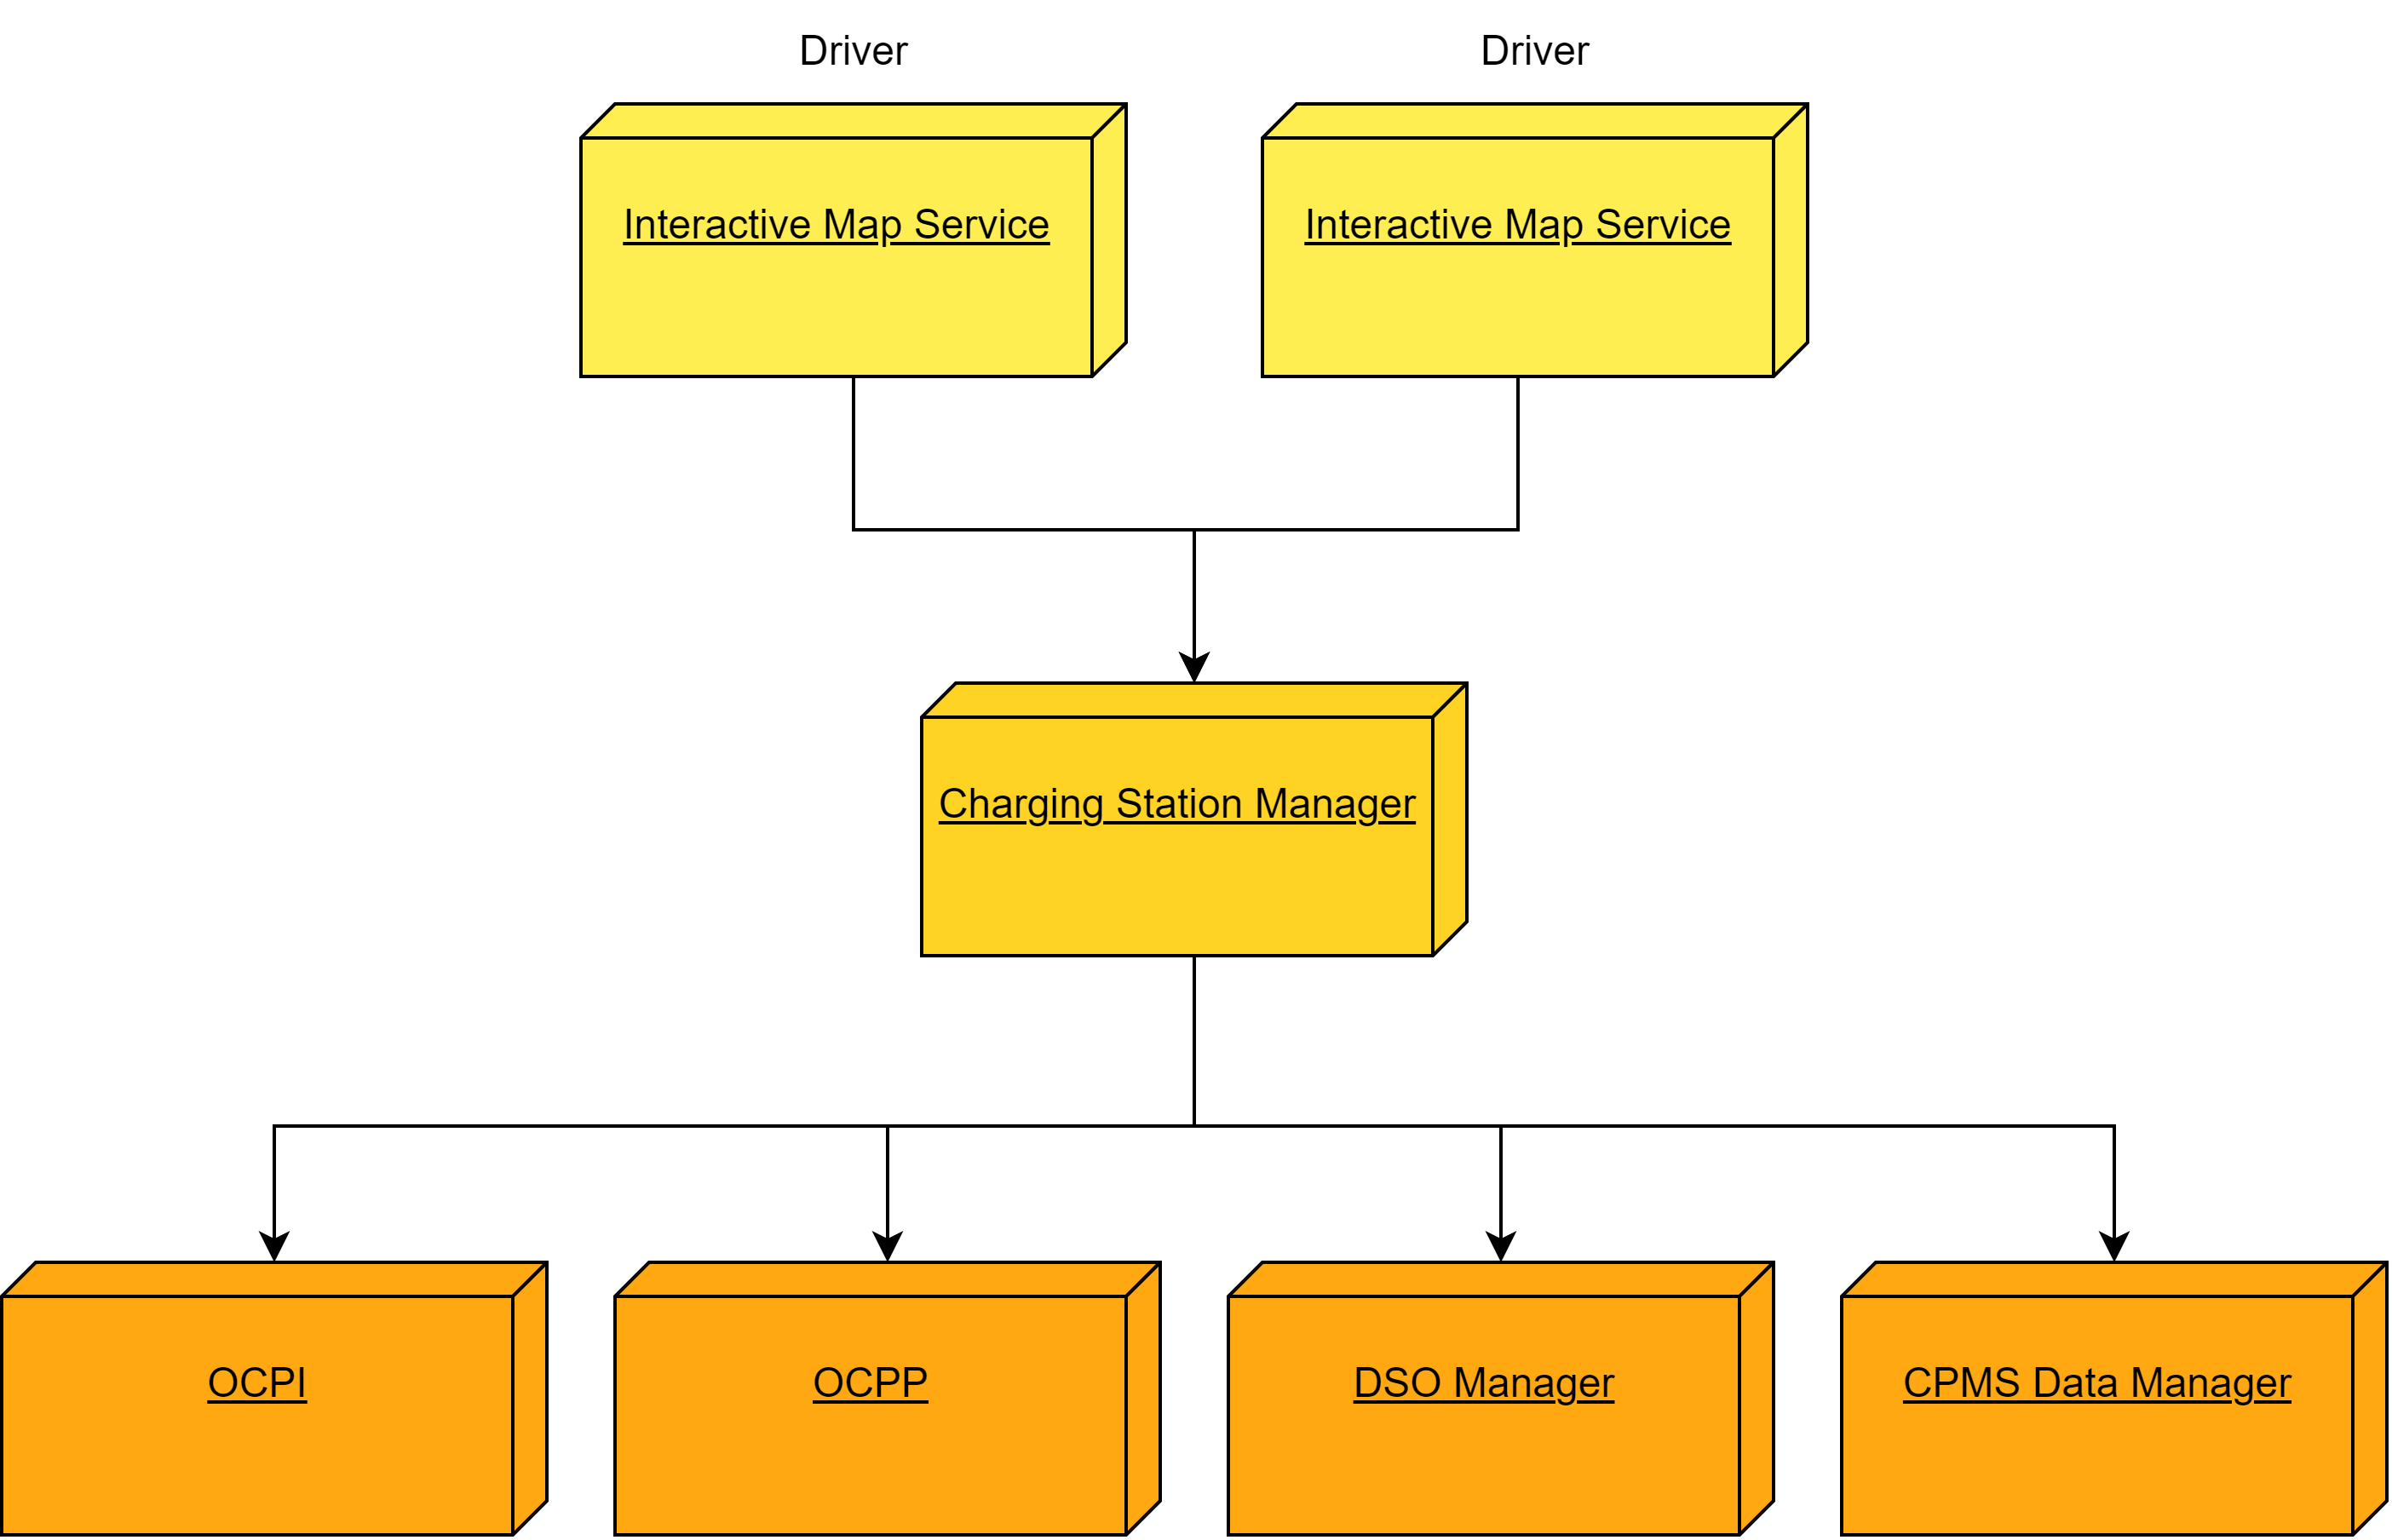
\includegraphics[scale=0.6]{assets/Integration Diagrams/CPMS-Charging Station Manager.png} 
    \caption{Integration of CPMS-Charging Station Manager}%
    \label{fig: CPMS-Charging Station Manager}%
\end{figure}

Lastly, are \emph{Account Manager} and \emph{CPOW Manager}, the two components that contain services. Note that at this point of development, drivers are no longer needed:

\begin{figure}[H]
    \centering
    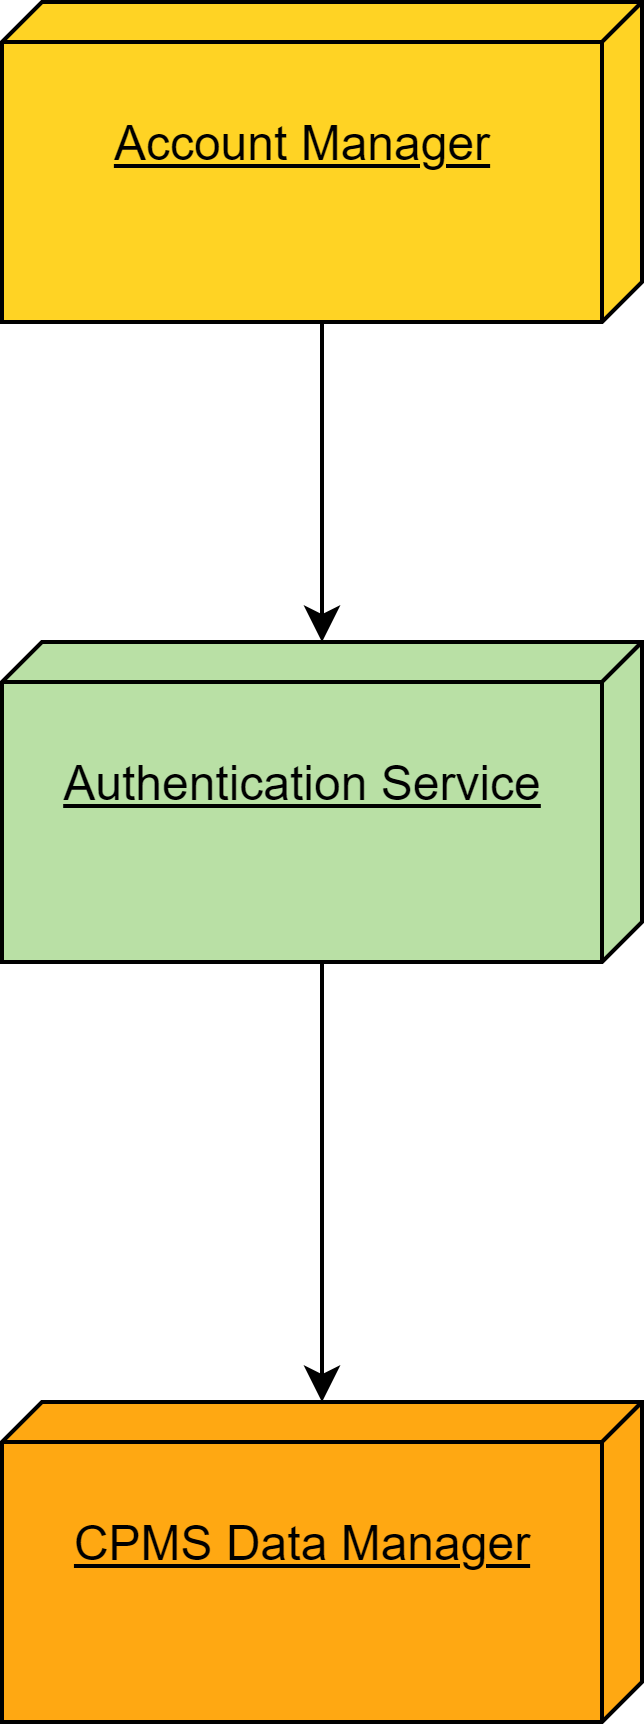
\includegraphics[scale=0.6]{assets/Integration Diagrams/CPMS-Account Manager.png} 
    \caption{Integration of CPMS-Account Manager}%
    \label{fig: CPMS-Account Manager}%
\end{figure}

\begin{figure}[H]
    \centering
    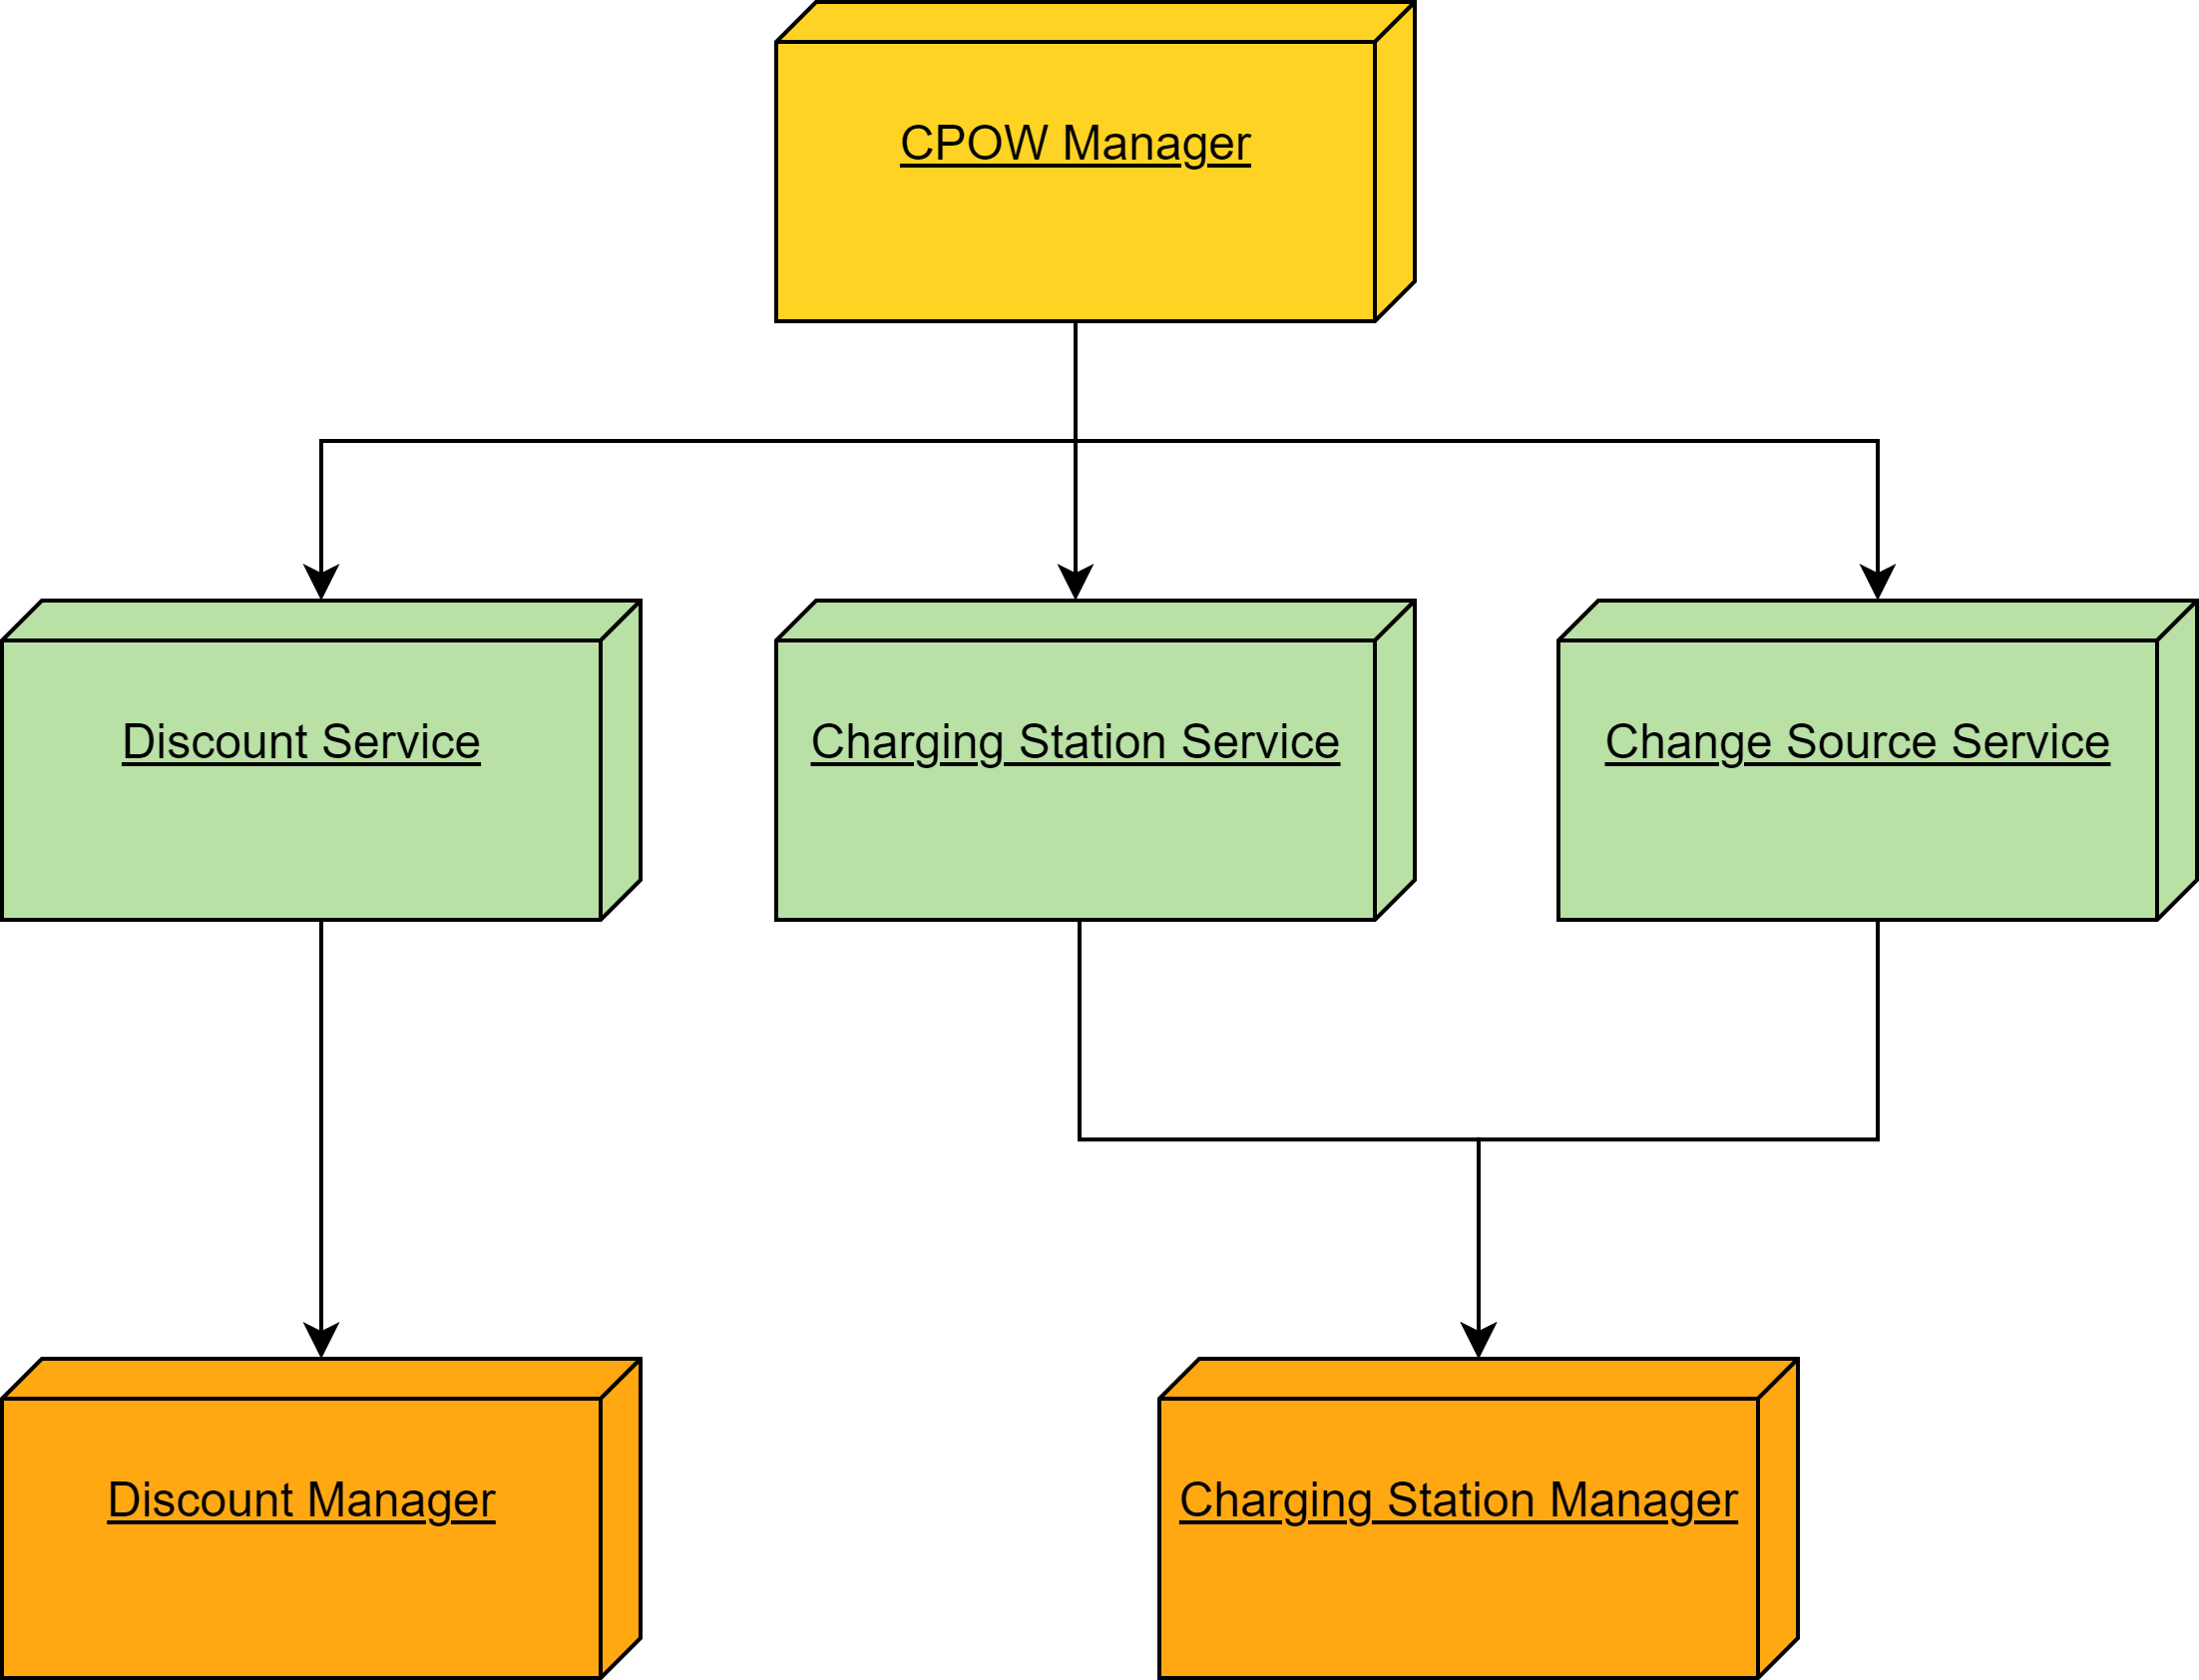
\includegraphics[scale=0.6]{assets/Integration Diagrams/CPMS-CPOW Manager.png} 
    \caption{Integration of CPMS-CPOW Manager}%
    \label{fig: CPMS-CPOW Manager}%
\end{figure}



\subsection{System testing}
Once specific testing for each component is done, and everything works, it is time to test the system as a whole. It is fundamental to thoroughly test a system before it is deployed, as this can help to identify and fix any issues that may impact the system's functionality or user experience.
For these reasons, some tests must be run to evaluate the system's performance, stability, security, and usability. Among these an important step would be testing the system's performance; especially in conditions
of high workload, to see if it is able to handle many requests at once. For example, it is important to check whether at midnight, when checks for user schedules are being done, other parts of the system suffer from a drop in performance.
Given the potentially large user base, usability testing would also be required. For example the application could be submitted to a number of candidates to check whether the application is intuitive and 
the use feels natural. In case of bad reception, an UI revamp might be done and some form of onboarding may be added.






\newpage
\section{Effort Spent}
    \begin{tabular}{|c||c|c|c|c|c|}
        \hline
        Student & Time for S.1 & S.2 & S.3 & S.4 & S.5\\ \hline
        stud1 & 0h & 0h & 0h & 0h & 0h \\
        stud2 & 0h & 0h & 0h & 0h & 0h \\
        stud3 & 0h & 0h & 0h & 0h & 0h \\
        \hline
    \end{tabular}


\section{References}


\begin{thebibliography}{9}
    \bibitem{reference1}
    MDN Web Docs Glossary: Definitions of Web-related terms -> MVC
    \url{https://developer.mozilla.org/en-US/docs/Glossary/MVC}

    \bibitem{reference2}
    description: \url{url here}
    
\end{thebibliography}

\end{document}